% !TEX program = xelatex
\documentclass[12pt, a4paper, openany]{book}

\usepackage{amsmath}
\usepackage{fontspec}
\usepackage{unicode-math}

\setmainfont{Bookman_Old_Style_Regular.ttf}[
    Path           = {./fonts/},
    BoldFont       = Bookman_Old_Style_Bold.ttf,
    ItalicFont     = Bookman_Old_Style_Italic.ttf,
    BoldItalicFont = Bookman_Old_Style_Bold_Italic.ttf
]
\setmathfont{TeX Gyre Schola Math}

\AtBeginDocument{
  \let\square\mdlgwhtsquare
  \let\Box\mdlgwhtsquare
}

\usepackage{titlesec}
\assignpagestyle{\part}{empty}

% ==========================================
% 1. НАСТРОЙКА ЧАСТЕЙ (\part)
% ==========================================
\titleformat{\part}[display]
  {\normalfont\Huge\bfseries\centering}
  {\partname~\thepart.}
  {20pt}
  {}
 [\clearpage]

\titlespacing*{\part}{0pt}{50pt}{40pt}

% ==========================================
% 2. НАСТРОЙКА ГЛАВ (\chapter)
% ==========================================
\titleformat{\chapter}[block]
  {\normalfont\Large\bfseries}
  {\thechapter.}
  {0.5em}
  {}

\titlespacing*{\chapter}{0pt}{-20pt}{40pt}

% ==========================================
% 3. НАСТРОЙКА ПАРАГРАФОВ (\section)
% ==========================================
\titleformat{\section}[block]
  {\normalfont\large\bfseries}
  {\thesection.}
  {0.5em}
  {}

\titlespacing*{\section}{0pt}{3.5ex plus 1ex minus .2ex}{2.3ex plus .2ex}

% ==========================================
% 4. НАСТРОЙКА ПОДПАРАГРАФОВ (\subsection)
% ==========================================
\titleformat{\subsection}[block]
  {\normalfont\normalsize\bfseries}
  {\thesubsection.}
  {0.5em}
  {}

\titlespacing*{\subsection}{0pt}{3.25ex plus 1ex minus .2ex}{1.5ex plus .2ex}

\usepackage{csquotes}
\usepackage[english, russian, ukrainian]{babel}

\usepackage{geometry}
\geometry{margin=2.5cm}

\usepackage[psdextra]{hyperref}

\hypersetup{
    bookmarksnumbered=true,
    colorlinks=true,
    linkcolor=darkgraylink,
    urlcolor=blue,
    citecolor=green!50!black,
    linktoc=page,
}

\usepackage{microtype}
\usepackage{booktabs}
\usepackage{enumitem}
\usepackage{xcolor}
\usepackage{mdframed}
\usepackage{graphicx}
\graphicspath{{pictures}}
\usepackage{tabularray}
\UseTblrLibrary{booktabs}
\usepackage{minted}
\setminted{
    fontsize=\scriptsize,
    bgcolor=gray!5,
    frame=lines,
    framesep=3mm,
    breaklines,
    autogobble=false,
    obeytabs=true,
    tabsize=4,
    showtabs=false,
}

\usepackage{caption}
\captionsetup{font=small, labelfont=bf}

\usepackage{bookmark}

\definecolor{boxbg}{RGB}{245,245,250}
\definecolor{accent}{RGB}{30,80,160}
\definecolor{planckblue}{RGB}{31,119,180}
\definecolor{theoryred}{RGB}{214,39,40}
\definecolor{darkgraylink}{RGB}{80, 85, 90}

\usepackage{pgfplots}
\pgfplotsset{compat=1.18}
\usepackage{pgfplotstable}

\usetikzlibrary{decorations.text}

\usepackage{indentfirst}

\usepackage[backend=biber,
            style=phys,
            sorting=none,
            maxnames=4,
            eprint=true,
            autolang=other,
            doi=true]{biblatex}

\addbibresource{references/references.bib}

\usepackage[most, many]{tcolorbox}

\newtcolorbox{mathbox}[2][]{
  enhanced,
  breakable,
  parbox=false,
  colback=theoryred!3,
  colframe=theoryred,
  sharp corners,
  boxrule=0pt,
  left=12pt, right=12pt, top=14pt, bottom=10pt,
  fontupper=\footnotesize,
  fonttitle=\small\bfseries\itshape,
  colbacktitle=theoryred!3,
  coltitle=theoryred!80!black,
  title={#2},
  overlay unbroken and first={
    \draw[theoryred!60, line width=0.4pt]
      ([xshift=2pt, yshift=-2pt]frame.north west) rectangle ([xshift=-2pt, yshift=2pt]frame.south east);
    \draw[theoryred, line width=1.2pt]
      ([xshift=5pt, yshift=-5pt]frame.north west) -- ([xshift=5pt, yshift=5pt]frame.south west);
    \draw[theoryred, line width=0.8pt] ([xshift=3pt, yshift=-5pt]frame.north west) -- ([xshift=9pt, yshift=-5pt]frame.north west);
    \draw[theoryred, line width=0.8pt] ([xshift=3pt, yshift=5pt]frame.south west) -- ([xshift=9pt, yshift=5pt]frame.south west);
  },
  overlay middle={
    \draw[theoryred!60, line width=0.4pt] (frame.north west) -- (frame.south west);
    \draw[theoryred!60, line width=0.4pt] (frame.north east) -- (frame.south east);
  },
  overlay last={
    \draw[theoryred!60, line width=0.4pt] (frame.north west) -- (frame.south west);
    \draw[theoryred!60, line width=0.4pt] (frame.north east) -- (frame.south east);
  },
  #1
}

\newtcolorbox{keybox}[2][]{
  enhanced,
  breakable,
  parbox=false,
  colback=boxbg,
  colframe=accent,
  sharp corners,
  boxrule=0pt,
  left=12pt, right=12pt, top=14pt, bottom=10pt,
  fontupper=\footnotesize,
  fonttitle=\small\bfseries\itshape,
  colbacktitle=boxbg,
  coltitle=accent!80!black,
  title={#2},
  overlay unbroken and first={
    \draw[accent!60, line width=0.4pt]
      ([xshift=2pt, yshift=-2pt]frame.north west) rectangle ([xshift=-2pt, yshift=2pt]frame.south east);
    \draw[accent, line width=1.2pt]
      ([xshift=5pt, yshift=-5pt]frame.north west) -- ([xshift=5pt, yshift=5pt]frame.south west);
    \draw[accent, line width=0.8pt] ([xshift=3pt, yshift=-5pt]frame.north west) -- ([xshift=9pt, yshift=-5pt]frame.north west);
    \draw[accent, line width=0.8pt] ([xshift=3pt, yshift=5pt]frame.south west) -- ([xshift=9pt, yshift=5pt]frame.south west);
  },
  overlay middle={
    \draw[accent!60, line width=0.4pt] (frame.north west) -- (frame.south west);
    \draw[accent!60, line width=0.4pt] (frame.north east) -- (frame.south east);
  },
  overlay last={
    \draw[accent!60, line width=0.4pt] (frame.north west) -- (frame.south west);
    \draw[accent!60, line width=0.4pt] (frame.north east) -- (frame.south east);
  },
  #1
}

\newcounter{problemcounter}[chapter]
\renewcommand{\theproblemcounter}{\arabic{chapter}.\arabic{problemcounter}}

\newtcolorbox{problemcontent}[2][]{
    enhanced,
    breakable,
    parbox=false,
    colback=gray!3,
    boxrule=0pt,
    sharp corners,
    left=22pt, right=10pt, top=8pt, bottom=8pt,
    before skip=14pt, after skip=14pt,
    fontupper=\footnotesize,
    colbacktitle=gray!3,
    title={},
    attach title to upper,
    overlay unbroken and first={
        \draw[black!40, line width=0.5pt] ([xshift=12pt, yshift=-4pt]frame.north west) -- ([xshift=12pt, yshift=4pt]frame.south west);
        \node[draw=black, fill=white, line width=0.6pt, inner sep=3pt, font=\scriptsize\bfseries\itshape, anchor=north]
            at ([xshift=5pt, yshift=-8pt]frame.north west) {№ #2};
    },
    overlay middle={
        \draw[black!40, line width=0.5pt] ([xshift=12pt]frame.north west) -- ([xshift=12pt]frame.south west);
    },
    overlay last={
        \draw[black!40, line width=0.5pt] ([xshift=12pt]frame.north west) -- ([xshift=12pt]frame.south west);
    },
    #1
}

\newenvironment{problem}[1]{
    \refstepcounter{problemcounter}
    \begin{problemcontent}{\theproblemcounter}
    {\bfseries\itshape #1}
}{
    \end{problemcontent}
}

\pgfplotstableread{data/plankdata.txt}\planckdata
\pgfplotstableread{data/LCDM.txt}\theorydata

% ==========================================
% ПОЧАТОК ДОКУМЕНТА ТА СТРУКТУРИ
% ==========================================
\begin{document}

% --- КАНОНІЧНА СТАРОВИННА ТИТУЛЬНА СТОРІНКА ---
\begin{titlepage}
    \centering
    \linespread{1.1}\selectfont

    \vspace*{0.5cm}
    % Верхня академічна частина (строга університетська капітель)
    {\scshape\large Національний технічний університет України \\[0.15cm]
    «Київський політехнічний інститут імені Ігоря Сікорського»} \\[0.4cm]
    {\large Фізико-технічний інститут} \\[0.15cm]
    {\small Кафедра прикладної фізики} \\

    \vfill

    % Велична подвійна рамка (Товста + Тонка лінія друкарського верстата)
    \rule{\textwidth}{1.6pt} \\[0.2cm]
    \rule{\textwidth}{0.6pt} \\[0.6cm]

    % НАЗВА КНИГИ (Великий, канонічний Bookman)
    {\Huge\bfseries Нотатки: від інфлатона до CMB} \\[0.6cm]

    \rule{\textwidth}{0.6pt} \\[0.2cm]
    \rule{\textwidth}{1.6pt} \\

    \vfill

% --- ЦЕНТРАЛЬНИЙ БЛОК: ГРАВЮРА ФЛАММАРІОНА ---
    % Картинка центрована, а невелика тонка рамка підкреслює ретро-ефект
    \begin{minipage}{0.55\textwidth}
        \centering
        \vspace*{0.2cm}
        \label{fig:flammarion_title}
        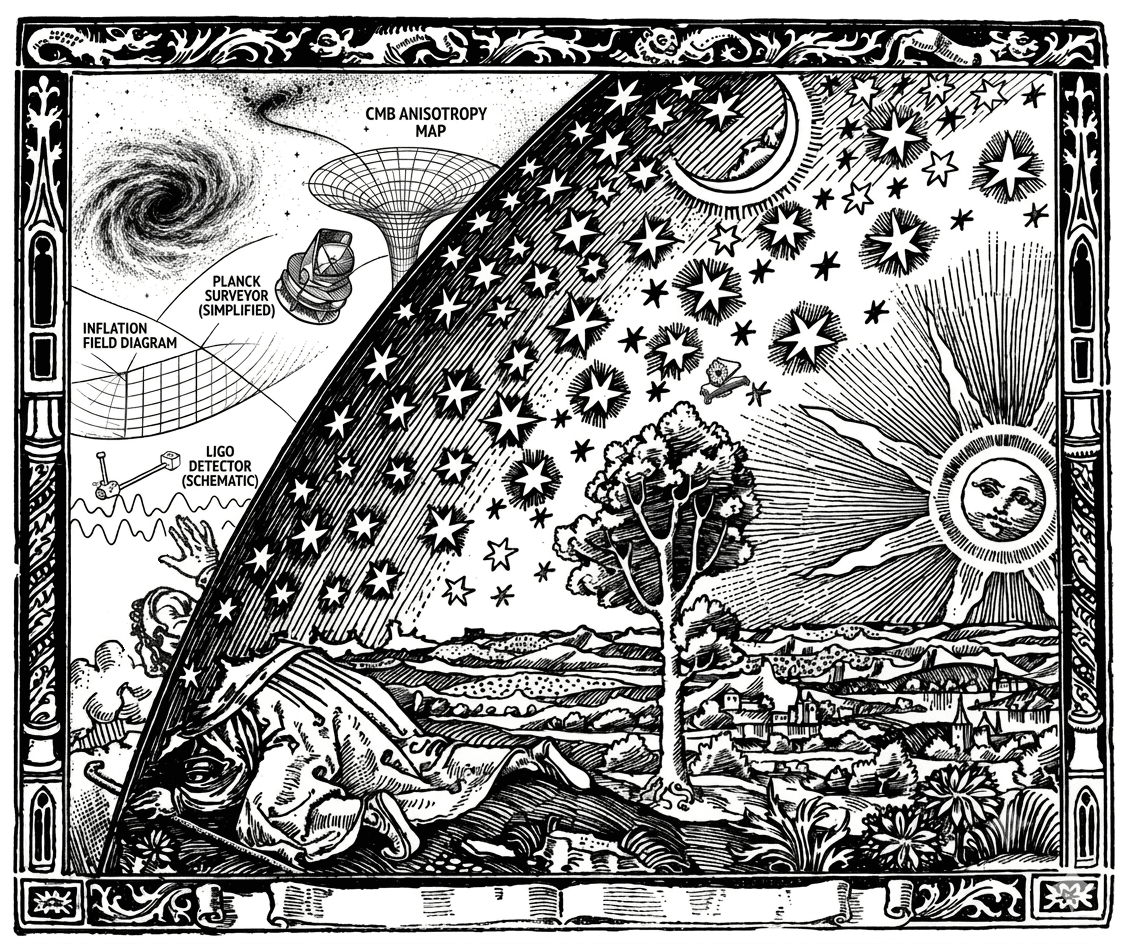
\includegraphics[width=\textwidth]{Modern_flagmarion}
        \vspace*{0.2cm}
    \end{minipage}

%    % --- СТИЛІЗОВАНА АСТРОНОМІЧНА ГРАВЮРА (ВИПРАВЛЕНИЙ TIKZ) ---
%    \begin{tikzpicture}[scale=0.75, every node/.style={transform shape}]
%        % Зовнішнє градусне коло
%        \draw[line width=0.8pt, darkgraylink] (0,0) circle (2.8cm);
%        \draw[line width=0.4pt, darkgraylink] (0,0) circle (2.6cm);
%        \draw[line width=0.4pt, dashed, darkgraylink] (0,0) circle (2.1cm);
%
%        % Напрямки осей та вимірювальні промені
%        \foreach \a in {0, 30, 60, 90, 120, 150, 180, 210, 240, 270, 300, 330} {
%            \draw[line width=0.3pt, darkgraylink!60] (\a:2.6cm) -- (\a:2.8cm);
%        }
%        \draw[line width=0.4pt, darkgraylink!50] (-3.2,0) -- (3.2,0);
%        \draw[line width=0.4pt, darkgraylink!50] (0,-3.2) -- (0,3.2);
%
%        % Внутрішні орбіти (еліпси)
%        \draw[line width=0.5pt, darkgraylink, rotate=15] (0,0) ellipse (1.6cm and 0.9cm);
%        \draw[line width=0.5pt, darkgraylink, rotate=-30] (0,0) ellipse (2.2cm and 1.2cm);
%
%        % Сонце в центрі (символ Інфляції / початку Всесвіту)
%        \draw[line width=0.6pt, fill=white, darkgraylink] (0,0) circle (0.35cm);
%        \foreach \a in {0, 45, 90, 135, 180, 225, 270, 315} {
%            \draw[line width=0.5pt, darkgraylink] (\a:0.35cm) -- (\a:0.65cm);
%        }
%
%        % Планети на орбітах (тепер через правильні node)
%        \node[draw, fill=white, circle, inner sep=1.2pt, line width=0.5pt, darkgraylink] at (15:1.6cm) {};
%        \node[draw, fill=white, circle, inner sep=1.5pt, line width=0.5pt, darkgraylink] at (-30:2.2cm) {};
%    \end{tikzpicture}

    \vfill

    % АВТОР
    {\Large\scshape Пономаренко С. М.} \\

    \vfill

    % Ромбовидна анотація старої школи для ідеального заповнення простору
    \begin{minipage}{0.8\textwidth}
        \centering\small\itshape
        Систематизовані нотатки з теоретичної космології, що охоплюють
        фізику раннього Всесвіту, динаміку скалярного інфлатонного поля,
        генерацію первинних космологічних збурень та їхній відбиток
        на анізотропії реліктового випромінювання (CMB).
    \end{minipage}

    \vfill\vfill

    % Нижній видавничий блок
    \rule{4cm}{0.5pt} \\[0.3cm]
    {\large\scshape Київ} \\[0.15cm]
    {\small 2026}

    \vspace*{0.5cm}
\end{titlepage}

\clearpage
% -------------------------------------------------------

\tableofcontents
\pagestyle{plain}

%% --------------------------------------------------------
\chapter*{Передмова}
\addcontentsline{toc}{chapter}{Передмова}
%% --------------------------------------------------------

Цей конспект будує міст між двома точками: \emph{інфлатоном}~---
гіпотетичним скалярним полем, яке керувало першими
${\sim}10^{-32}$~с існування Всесвіту~--- і \emph{реліктовим випромінюванням} (CMB),
що є найдетальнішою спостережуваною картиною того, що відбулося.
Між цими точками лежить ланцюжок物理, який ми будуємо
послідовно, крок за кроком.

\textbf{Частина~I. Фон.} Розділи~\ref{sec:friedmann}–\ref{sec:inflaton}
закладають геометричну та динамічную основу: рівняння Фрідмана описують
однорідний і ізотропний Всесвіт, що розширюється; інфлатон і його
потенціал $V(\phi)$ пояснюють, чому це розширення на початку було
прискореним (інфляція). Цей ідеалізований, полностью симетричний фон є
\emph{нульовим наближенням}, на якому тримається вся подальша фізика.

\textbf{Частина~II. Збурення.} Розділи~\ref{sec:metric}-\ref{sec:quantum}
переходять від симетричного фону до реального світу. Квантові флуктуації
інфлатона~--- неминучі за принципом невизначеності~--- стають
\emph{насінням} усієї великомасштабної структури. Тензорні збурення
метрики народжують первинні гравітаційні хвилі. Розділ~\ref{sec:metric}
формалізує мову, якою описуються ці збурення: SVT-розклад і
конформно-ньютонівське калібрування.

\textbf{Частина~III. Спостереження.} Розділи~\ref{sec:reheating}–\ref{sec:pol}
стежать за долею збурень після інфляції: розігрів перетворює поле на
гарячу плазму; акустичні осциляції цієї плазми залишають відбиток у
вигляді піків на спектрі CMB і масштабу BAO; поляризаційні E- і B-моди
несуть інформацію про скалярні та тензорні збурення відповідно.

\textbf{Частина~IV. Невирішені проблеми і шляхи їх пошуку.} Розділи~\ref{sec:chaotic}–\ref{sec:future_research}
виходять за межі стандартної моделі. Телескоп JWST виявив масивні
галактики при $z \sim 10$–$12$, існування яких важко узгодити зі
стандартним степенево-законним первинним спектром. Ми розглядаємо
механізм локального \emph{зламу спектра} через особливість у потенціалі
інфлатона і формулюємо програму перевірки цієї ідеї за допомогою
CAMB/CLASS та байєсівського аналізу (MCMC).

\bigskip
\noindent
\textit{Передумови.} Конспект розрахований на читача, знайомого із
загальною теорією відносності на рівні тензора Рімана і рівнянь
Айнштайна, та з квантовою теорією поля на рівні канонічного
квантування. Знання космології не передбачається.

\newpage

%% --------------------------------------------------------
\part{Фон}
%% --------------------------------------------------------
% !TeX root = ../Cosmology.tex

%% --------------------------------------------------------
\chapter{Фонова космологія: від метрики FLRW до $\Lambda$CDM}
\label{sec:friedmann}
%% --------------------------------------------------------

Космологія описує Всесвіт як єдиний фізичний об'єкт. Її фундаментальним
відправним пунктом є \textbf{космологічний принцип} (принцип однорідності та ізотропії):
на достатньо великих просторових масштабах ($\gtrsim 100$~Мпк) розподіл
матерії та геометрія простору-часу є трансляційно та ротаційно інваріантними, тобто
не виділяють жодного напрямку і жодної точки. Цей симетрійний постулат
жорстко фіксує єдиний допустимий клас геометрій~--- метрику
Фрідмана--Леметра--Робертсона--Вокера (FLRW)~--- і зводить систему тензорних
рівнянь Айнштайна до двох звичайних диференціальних рівнянь для однієї скалярної
функції часу~--- \textbf{масштабного фактора} $a(t)$.
Фізичний зміст $a(t)$ простий: якщо сьогодні ($t = t_0$) дві галактики
розділені відстанню $d_0$, то в момент $t$ відстань між ними була
$d(t) = a(t)\,d_0/a(t_0)$.
Нормуємо $a(t_0) \equiv 1$: тоді $a < 1$ означає минуле
(Всесвіт менший), $a > 1$~--- майбутнє.

\medskip\noindent%
\textbf{Логічна карта розділу}
% ------------------------------
% Логічна карта розділу 1 (фонова космологія)
% ------------------------------
\begin{center}
\begin{tikzpicture}[roadmap]

\node[box] (FLRW) {Метрика FLRW};
\node[box, right=of FLRW] (Friedmann) {Рівняння\\ Фрідмана};
\node[box, right=of Friedmann] (EOS) {Рівняння\\ стану};
\node[box, right=of EOS] (LCDM) {$\Lambda$CDM};
\node[box, right=of LCDM, fill=red!5, draw=red!70!black] (problems) {Проблеми};

\draw[arrow] (FLRW) -- (Friedmann);
\draw[arrow] (Friedmann) -- (EOS);
\draw[arrow] (EOS) -- (LCDM);
\draw[arrow] (LCDM) -- (problems);

% Підписи зверху
\node[font=\tiny\bfseries, text=blue!70!black, above=0.1cm of FLRW, align=center] {Однорідність\\ та ізотропія};
\node[font=\tiny\bfseries, text=blue!70!black, above=0.1cm of Friedmann, align=center] {Динаміка $a(t)$};
\node[font=\tiny\bfseries, text=blue!70!black, above=0.1cm of EOS, align=center] {$w = p/(\rho c^2)$};
\node[font=\tiny\bfseries, text=blue!70!black, above=0.1cm of LCDM, align=center] {Плоский\\ Всесвіт};
\node[font=\tiny\bfseries, text=red!70!black, above=0.1cm of problems, align=center] {Що не так?};

% Пояснення знизу
\node[font=\scriptsize, gray, below=0.1cm of FLRW] {$ds^2 = -c^2dt^2 + a^2\delta_{ij}dx^idx^j$};
\node[font=\scriptsize, gray, below=0.1cm of Friedmann] {$H^2 = \frac{8\pi G}{3}\rho$};
\node[font=\scriptsize, gray, below=0.1cm of EOS] {$\rho \propto a^{-3(1+w)}$};
\node[font=\scriptsize, gray, below=0.1cm of LCDM] {$\Omega_m + \Omega_\Lambda = 1$};
\node[font=\scriptsize, gray, below=0.1cm of problems, align=center] {плоскість, \\горизонт, збурення};

\end{tikzpicture}
\end{center}

Метрика FLRW у \emph{космологічному (власному) часі}~$t$ для загального випадку
тривимірного простору з постійною кривизною $k = \pm 1, 0$ записується як:
\begin{equation}\label{eq:FLRW_general}
  ds^2 = -c^2 dt^2 + a(t)^2 \left[ \frac{dr^2}{1 - kr^2} + r^2(d\theta^2 + \sin^2\theta\,d\phi^2) \right].
\end{equation}
Для локально плаского Всесвіту ($k = 0$) метрика~\eqref{eq:FLRW_general} набуває спрощеного вигляду:
\begin{equation}\label{eq:FLRW}
  ds^2 = -c^2 dt^2 + a(t)^2\,\delta_{ij}\,dx^i dx^j.
\end{equation}

Підставляючи метричний тензор у рівняння Айнштайна
$G_{\mu\nu} + \Lambda g_{\mu\nu} = \dfrac{8\pi G}{c^4}\,T_{\mu\nu}$ та моделюючи космічний
субстрат як \textbf{ідеальну гідродинамічну рідину}, ми задаємо тензор
енергії-імпульсу у \textbf{супутній системі відліку}%
\footnote{Супутня система відліку~--- це система спостерігача, який
  «пливе» разом із космологічним розширенням, тобто має нульову пекулярну
  швидкість. У такій системі речовина локально перебуває у спокої, і
  тензор $T^{\mu}{}_\nu$ набуває діагонального вигляду.}
у діагональній формі:
\begin{equation*}
  T^\mu{}_\nu = \mathrm{diag}(-\rho c^2,\,p,\,p,\,p).
\end{equation*}
Знак мінус перед $\rho c^2$ є наслідком сигнатури метрики $(-,+,+,+)$:
часова компонента $T^0{}_0 = -\rho c^2$ відповідає густині енергії,
просторові $T^i{}_j = p\,\delta^i{}_j$ --- ізотропному тиску.
Обчислення символів Крістофеля для метрики FLRW та згортка з тензором
Рімана дають ненульові компоненти тензора Айнштайна:
\begin{equation*}
  G^0{}_0 = -\frac{3H^2}{c^2} - \frac{3k}{a^2},
  \qquad
  G^i{}_j = -\frac{1}{c^2}\!\left(2\dot H + 3H^2 + \frac{kc^2}{a^2}\right)\delta^i{}_j,
  \qquad
  H \equiv \frac{\dot a}{a}.
\end{equation*}
Величина $H(t)$ називається \textbf{параметром Хаббла}, вона
є ключовою характеристикою космологічної кінематики і визначає
миттєвий темп розширення Всесвіту.

Підставляючи ці вирази у рівняння Айнштайна, отримуємо систему
\textbf{рівнянь Фрідмана}:
\begin{subequations}\label{eq:friedmann_system}
\begin{align}
  H^2 &= \frac{8\pi G}{3}\,\rho - \frac{kc^2}{a^2} + \frac{\Lambda c^2}{3},
  \label{eq:F1}\\[4pt]
  \frac{\ddot a}{a} &= -\frac{4\pi G}{3}\,\left(\rho + \frac{3p}{c^2}\right) + \frac{\Lambda c^2}{3},
  \label{eq:F2}\\[4pt]
  \dot\rho &= -3H\left(\rho + \frac{p}{c^2}\right).
  \label{eq:conservation_law}
\end{align}
\end{subequations}
Перше~\eqref{eq:F1} --- енергетичний баланс ($(00)$-компонента);
друге~\eqref{eq:F2} --- динаміка прискорення ($(ii)$-компонента).
Третє~\eqref{eq:conservation_law} --- космологічний аналог першого
закону термодинаміки: для однорідної сферичної області об'єму
$V \propto a^3$ воно відтворює $dE = -p\,dV$, де $E = \rho c^2 V$
(детальніше~--- дод.~\ref{app:newton_energy}).
Зауважимо, що~\eqref{eq:conservation_law} не є незалежним: воно
автоматично випливає з~\eqref{eq:F1} і~\eqref{eq:F2} через
тотожність Б'янкі $\nabla_\mu G^{\mu\nu} = 0$.
Система~\eqref{eq:friedmann_system} має рівно \emph{два} незалежних
ступені свободи, але третє рівняння зручніше для безпосереднього
інтегрування і широко використовується надалі.

Для точного математичного моделювання реального Всесвіту ми маємо враховувати одночасний внесок усіх його фізичних компонентів. Прирівнюючи перше рівняння Фрідмана~\eqref{eq:F1} до нуля при $k = 0$ та $\Lambda = 0$, ми визначаємо \textbf{критичну густину}~--- густину, якій відповідає геометрично плоский Всесвіт,~--- та пов'язані з нею безрозмірні параметри густини~$\Omega_i$:
\begin{equation}\label{eq:rho_crit_new}
  \rho_\text{cr}(t) \equiv \frac{3H^2(t)}{8\pi G}, \qquad
  \Omega_i(t) \equiv \frac{\rho_i(t)}{\rho_{\rm cr}(t)}, \qquad
  \Omega_\Lambda(t) \equiv \frac{\Lambda c^2}{3H^2(t)}.
\end{equation}

Поділивши перше рівняння Фрідмана на $H^2(t)$, ми можемо записати його у безрозмірній формі через введені параметри $\Omega_i$. При цьому геометричний член кривизни $-kc^2/(a^2 H^2)$ космологи часто формально трактують як внесок від специфічного «квазіматеріального» флюїду, вводячи \textbf{параметр густини кривизни} $\Omega_k$:
\begin{equation}\label{eq:Omega_k_def}
  \Omega_k(t) \equiv -\frac{kc^2}{a^2(t)H^2(t)}.
\end{equation}
З погляду загальної теорії відносності кривизна $k$ є чистою властивістю просторової геометрії і не є матеріальним джерелом. Проте такий математичний трюк дозволяє звести рівняння Фрідмана для довільної топології простору до елегантного алгебраїчного інваріанта:
\begin{equation}\label{eq:omega_sum}
  \sum \Omega_i(t) + \Omega_k(t) = 1,
\end{equation}
де сума береться за всіма реальними фізичними компонентами (радіація, баріони, холодна темна матерія). Якщо Всесвіт є суворо пласким ($k=0$), то $\Omega_k \equiv 0$, а сума густин речовини та темної енергії точно дорівнює одиниці. Натомість у закритому Всесвіті ($k = +1$, сфера) цей ефективний флюїд має від'ємну густину ($\Omega_k < 0$) та ефективне рівняння стану $w_k = -1/3$, а його густина згасає з розширенням як $\rho_k \propto a^{-2}$.

Використовуючи ці визначення, ми можемо переписати перше рівняння Фрідмана~\eqref{eq:F1} у загальному вигляді критерію енергетичного балансу~\cite{Weinberg2008,Baumann2022}:
\begin{equation}\label{eq:omega_sum_k_integrated}
  \sum_i \Omega_i(t) - 1 = \frac{kc^2}{a^2 H^2} \equiv -\Omega_k(t),
\end{equation}
де $\sum_i \Omega_i(t) = \Omega_m(t) + \Omega_r(t) + \Omega_\Lambda(t)$~---
сума внесків матерії, випромінювання і темної енергії
(космологічна стала трактується як компонента з $w=-1$).
Сучасні дані~\cite{planck_2018} дають $|\Omega_k| < 0.005$,
тобто Всесвіт є геометрично плоским з високою точністю.

\begin{keybox}{Геометрична vs динамічна плоскість}
Важливо розрізняти два питання.
\textbf{Геометричне:} яке значення $k$?
Параметр $k = 0, \pm1$ є глобальною топологічною характеристикою
простору~--- її точне значення невідоме і принципово
не може бути встановлено зі спостережень у межах
скінченного горизонту частинок.
\textbf{Динамічне:} наскільки ця кривина \emph{відчутна}
на доступних нам масштабах?
Це вимірює $\Omega_k(t) = -kc^2/(a^2H^2)$~---
величина, що залежить від часу через $a(t)$.

Якщо $k \neq 0$ але $a^2H^2 \gg c^2$, то $|\Omega_k| \ll 1$~---
кривина існує, але радіус кривини $R_{\rm curv} = a/\sqrt{|k|}$
настільки перевищує горизонт Хаббла $c/H$, що в межах
спостережуваного Всесвіту геометрія є практично евклідовою.
Аналогія: поверхня Землі сферична ($k=+1$), але на масштабі
міста виглядає плоскою.

Тому коли ми кажемо \enquote{Всесвіт плаский}~--- ми маємо на увазі
$|\Omega_k(t_0)| < 0.005$, а не обов'язково $k = 0$.
Різниця принципова концептуально, але не практично:
для всіх розрахунків $k = 0$ є бездоганним
наближенням.
\end{keybox}


%% --------------------------------------------------------
\section{Рівняння стану і закони розширення}
\label{sec:eos}
%% --------------------------------------------------------

Динамічна еволюція кожної космічної компоненти повністю визначається
її \textbf{рівнянням стану} $w \equiv p/(\rho c^2)$. За умови сталого $w$
рівняння збереження~\eqref{eq:conservation_law} інтегрується аналітично:
\begin{equation}\label{eq:rho_evolution}
  \rho(a) = \rho_0 \left(\frac{a_0}{a}\right)^{3(1+w)},
\end{equation}
а підстановка у~\eqref{eq:F1} дає кінематичний закон ($w \neq -1$):
\begin{equation}\label{eq:a_evolution}
  a(t) \propto t^{\,\frac{2}{3(1+w)}}.
\end{equation}

Для повноти картини зведемо основні космологічні епохи до таблиці~\ref{tab:epochs}. У ній наведено лише ті компоненти, які домінують у різні періоди
еволюції Всесвіту. Відсутня, зокрема, \textbf{інфляційна епоха}
($w \approx -1$), оскільки вона передує гарячій стадії і буде
розглянута окремо в наступному розділі~\ref{sec:inflation_kinematics}.

\begin{table}[h!]
\centering\small
\caption{Зведена таблиця космологічних епох: рівняння стану~$w$, закон еволюції густини~$\rho(a)$ та масштабного фактора $a(t)$ часі}
\label{tab:epochs}
\begin{tblr}{
  colspec={Q[l,m]X[l,m]Q[l,m]Q[l,m]Q[l,m]Q[l,m]},
  row{1} = {c, m, font=\bfseries},
}
\toprule
Епоха & Джерело маси-енергії & $w$ & $\rho(a)$ & $a(t)$ \\
\midrule
Радіаційна
  & Фотони, релятивістські нейтрино
  & $1/3$
  & $\propto a^{-4}$
  & $\propto t^{1/2}$ \\
Матеріальна
  & Холодна темна матерія + баріони
  & $0$
  & $\propto a^{-3}$
  & $\propto t^{2/3}$ \\
Сьогодні
  & Темна енергія ($\Lambda$-член)
  & $-1$
  & $\mathrm{const}$
  & $\propto e^{Ht}$ \\
\bottomrule
\end{tblr}
\end{table}

Член кривини $\Omega_k$ формально відповідає ефективному флюїду з $w_k = -1/3$ і густиною $\rho_k \propto a^{-2}$, однак він не є самостійною матеріальною компонентою, а виникає з геометрії простору.

%% --------------------------------------------------------
\section{Конформний час}
\label{sec:horizon}
%% --------------------------------------------------------

Динамічна природа Всесвіту FLRW створює серйозний концептуальний виклик для опису його еволюції: оскільки тканина простору неперервно розширюється, класичний фізичний (космічний) час $t$, який вимірюється годинником локально нерухомого спостерігача, виявляється вкрай незручним для аналізу глобальних процесів. Головна проблема полягає в тому, що швидкість світла $c$ є константою лише локально, тоді як на великих масштабах фотони змушені подорожувати простором, який постійно \enquote{втікає} з-під них. Як наслідок, на стандартних просторово-часових діаграмах $(t, r)$ траєкторії світлових променів (світлові конуси) стають складними викривленими лініями, залежними від еволюції густини енергії. Це суттєво заплутує аналіз причинно-наслідкової структури та причинних горизонтів.

Щоб повернути простору-часу геометричну простоту та інтуїтивну наочність, у космології здійснюють перехід до \emph{конформного часу} $\eta$. Математично конформний час визначається диференціальним співвідношенням, яке повністю компенсує часову зміну масштабного фактора $a(t)$:
\begin{equation}\label{eq:conformal_time_def}
  d\eta = \frac{dt}{a(t)}.
\end{equation}
У цих нових змінних просторово-пласка ($k=0$)\footnote{Вибір $k=0$ обґрунтовується спостереженнями: дані
\emph{Planck}~\cite{planck_2018} свідчать, що геометрія Всесвіту
є плоскою з точністю до $\sim 1\%$.} метрика FLRW набуває елегантного конформно-пласького вигляду:
\begin{equation}\label{eq:conformal_metric}
  ds^2 = a^2(\eta)\bigl(-c^2 d\eta^2 + \delta_{ij}\,dx^i dx^j\bigr).
\end{equation}

Фізично цей новий «космічний годинник» можна уявити так: оскільки $d\eta = dt/a$, в ранню епоху малого $a$ один «тік» конформного годинника охоплює дуже короткий фізичний інтервал $dt = a\,d\eta \ll d\eta$. Конформний час таким чином «розтягує» ранню еволюцію Всесвіту і дозволяє однаково детально описувати як стрімкі процеси ранньої плазми, так і повільну пізню динаміку~--- без зміни форми рівнянь.

\noindent\textbf{Фізичні та математичні переваги конформного формалізму.}
Рівняння~\eqref{eq:conformal_metric} показує, що вся динаміка розширення Всесвіту тепер повністю \enquote{захована} у загальному конформному множнику $a^2(\eta)$, який стоїть перед дужками, тоді як геометрія всередині дужок залишається абсолютно тотожною статичному простору Мінковського. Це дає дві ключові переваги для моделювання космології:
\begin{enumerate}
    \item \textbf{Стабільна причинна структура:} Оскільки для фотонів інтервал руху завжди $ds^2 \equiv 0$, з виразу всередині дужок~\eqref{eq:conformal_metric} прямо випливає закон радіального поширення світла: $c\,d\eta = d\chi$ (де $\chi$~--- супутня просторова координата\footnote{Точніше, $\chi$ --- це радіальна супутня координата, пов'язана з декартовими супутніми координатами $x^i$ співвідношенням $\chi = \sqrt{(x^1)^2 + (x^2)^2 + (x^3)^2}$. У випадку радіального руху світла ($d\theta = d\phi = 0$) просторова частина метрики зводиться саме до $d\chi^2$.}). Це означає, що на просторово-часових діаграмах у координатах $(\eta, \chi)$ світлові конуси завжди залишаються ідеальними прямими лініями під кутом $45^\circ$ (за умови однакового масштабу обох осей, тобто при відкладанні $c\eta$ і $\chi$ в одних одиницях), значно спрощуючи розрахунок причинних горизонтів.
    \item \textbf{Незмінна координатна сітка:} У конформному формалізмі розширення простору відображається як роздування самої координатної сітки. Через це «адреси» (супутні координати $\chi$) об'єктів, які беруть участь у загальному хаббловському потоці, залишаються константними. Реальні фізичні швидкості окремих об'єктів відносно цього фону~--- \emph{пекулярні швидкості} (від англ.\ \textit{peculiar}~--- особливий, власний)~--- відокремлюються від загального розширення і не входять у хаббловський потік. На космологічних масштабах ($\gtrsim 100$~Мпк) пекулярними швидкостями зазвичай нехтують; на локальних~--- вони принципові\footnote{Класичний приклад: галактика Андромеда (M31) наближається до Чумацького Шляху з пекулярною швидкістю ${\sim}110\,\text{км/с}$ завдяки локальному гравітаційному притяганню~--- попри загальне хаббловське розширення.}.
\end{enumerate}

%Розв'язуючи рівняння~\eqref{eq:calH_prime} для сталого $w$, ми знаходимо точні закони еволюції $a(\eta)$ для кожної космологічної епохи (табл.~\ref{tab:epochs}).


%% --------------------------------------------------------
\section{Космологічний червоний зсув та космологічні відстані}
\label{sec:redshift_distances}
%% --------------------------------------------------------

Маючи інструмент конформного часу і чітке розуміння причинної структури,
ми тепер можемо систематично описати як вимірюються відстані
у розширюваному Всесвіті~--- і чому у космології їх існує кілька.

Усі макроскопічні спостереження в астрофізиці пов'язані з динамікою
масштабного фактора $a(t)$ через безрозмірну величину~---
\textbf{космологічний червоний зсув}~$z$. Фотон, випромінений
джерелом у момент $t_e$, приходить до спостерігача в момент $t_0$
з розтягненням довжини хвилі:
\begin{equation}\label{eq:redshift}
  1 + z \equiv \frac{\lambda_{\rm obs}}{\lambda_{\rm em}}
             = \frac{a(t_0)}{a(t_e)}.
\end{equation}
При стандартному нормуванні $a(t_0) \equiv 1$ отримуємо
фундаментальний зв'я\-зок між геометрією та спостереженнями:
\begin{equation}\label{eq:a_z}
  a(t_e) = \frac{1}{1+z}.
\end{equation}
Це рівняння є ключем до космологічних вимірювань: воно дозволяє
замінити теоретичну координату $t_e$, яку неможливо виміряти без
апріорного знання моделі, на безпосередньо спостережуваний
спектроскопічний параметр~$z$.

Реперні значення $z$ в історії Всесвіту:
\begin{align*}
  z &= 0      && \text{(сьогодні, спостерігач)}, \\
  z &\approx 0.3  && \text{(початок прискореного розширення під дією $\Lambda$)}, \\
  z &\approx 1100 && \text{(рекомбінація, формування CMB)}, \\
  z &\sim 10^{10} && \text{(первинний нуклеосинтез)}.
\end{align*}

%% --------------------------------------------------------
\subsection*{Закон Хаббла}
%% --------------------------------------------------------

З відкриття Едвіна Габбла в 1929 році почалася сучасна космологія:
спостерігаючи далекі галактики, він виявив, що їхні спектри зміщені
в червоний бік, причому швидкість віддалення лінійно зростає з відстанню.
Сьогодні ми інтерпретуємо це як наслідок розширення самого простору.

У конформній метриці для плоского Всесвіту~\eqref{eq:conformal_metric}
супутні координати $x^i$ нерухомого спостерігача не змінюються з часом.
Відстань між двома точками вздовж просторової геодезичної в момент $t$
дорівнює добутку масштабного фактора на різницю їхніх супутніх координат:
$d_p(t) = a(t)\,\Delta \chi$. Позначаючи $d_C \equiv \Delta \chi$ (супутня
відстань), маємо:
\begin{equation}
d_p(t) = a(t)\,d_C.
\end{equation}

Диференціюючи цей вираз за часом, отримуємо:
\begin{equation}\label{eq:hubble_law}
\dot{d}_p = \frac{\dot{a}}{a}\,d_p = H(t)\,d_p, \qquad
H \equiv \frac{\dot{a}}{a}.
\end{equation}
Це і є \textbf{закон Хаббла} в диференціальній формі: швидкість
віддалення об'єкта пропорційна його відстані, а коефіцієнтом
пропорційності виступає параметр Хаббла.

Сьогодні ($t = t_0$) маємо $\dot{d}_p = H_0\,d_p$, де
$H_0 = 100\,h\,\text{км/с/Мпк}$ ($h = 0.6736$ за даними
\textit{Planck}~2018~\cite{planck_2018}).

Фізична відстань $d_p(t)$ є \emph{практично
неспостережуваною}. Вона змінюється щомиті через розширення простору,
тоді як світло фіксує об'єкт у минулому, а не в його теперішньому
положенні. Тому закон Хаббла в такому вигляді є лише кінематичним
співвідношенням, а не робочою формулою для вимірювань.

%% --------------------------------------------------------
\subsection*{Супутня відстань}
%% --------------------------------------------------------

Для фотона $ds^2 = 0$, тому з конформної метрики~\eqref{eq:conformal_metric}
випливає $c\,d\eta = d\chi$ (див.\ §\,\ref{sec:horizon}). Отже, супутня
відстань до об'єкта, що випромінив світло в момент $\eta_e$ (який ми
спостерігаємо в момент $\eta_0$), дорівнює:
\begin{equation*}
d_C \equiv \chi = c\int\limits_{\eta_e}^{\eta_0} d\eta'
           = c\int\limits_{t_e}^{t_0} \frac{dt}{a(t)}.
\end{equation*}

Величина $c\,dt/a(t)$ має просту інтерпретацію: це елемент
\textbf{супутньої відстані}, який світло проходить за фізичний час $dt$.
Обернена величина $a(t)/c$ визначає миттєвий \textbf{горизонт Хаббла}
$R_H(t) = c/H(t)$ (у фізичних координатах), який відокремлює області, що віддаляються повільніше або швидше
за швидкість світла.


\begin{keybox}{Конформний горизонт Хаббла}
У конформній метриці \eqref{eq:conformal_metric} природно ввести
конформний параметр Хаббла $\mathcal{H} \equiv a'/a = aH$ (штрих ---
похідна за $\eta$). Тоді конформний горизонт Хаббла дорівнює
\begin{equation*}
    c\mathcal{H}^{-1} = \frac{c}{aH}.
\end{equation*}

На відміну від звичайного радіуса Хаббла $R_H = c/H$, конформний горизонт $c\mathcal{H}^{-1}$ вимірюється в супутніх координатах. Це робить його зручним інструментом для порівняння фізичних масштабів космологічних структур (наприклад, BAO) із причинною структурою Всесвіту в будь-який момент часу.
\end{keybox}


Оскільки безпосередньо виміряти космічний час $t_e$ неможливо,
перейдемо до спостережуваного червоного зсуву $z$. Диференціюючи~\eqref{eq:a_z} отримуємо:
\begin{equation*}
\dot{a} = -\frac{1}{(1+z)^2}\,\dot{z}.
\end{equation*}

Підставляючи це у визначення параметра Хаббла $H \equiv \dot{a}/a$, маємо:
\begin{equation*}
    H = \frac{\dot{a}}{a} = (1+z) \cdot \left( -\frac{\dot{z}}{(1+z)^2} \right)
    = -\frac{1}{1+z}\,\frac{dz}{dt},
\end{equation*}
звідки знаходимо потрібний диференціал:
\begin{equation*}
d\eta = \frac{dt}{a(t)} = -\frac{dz}{H(z)}.
\end{equation*}

Далі необхідно знати явну залежність $H(z)$. Для цього розділимо
перше рівняння Фрідмана~\eqref{eq:F1} на $H_0^2$. Використовуючи безрозмірні параметри густини
$\Omega_i \equiv \rho_{i0}/\rho_{\rm cr0}$ та закон еволюції кожної
компоненти $\rho(a) = \rho_0 (a_0/a)^{3(1+w)}$ (див.~\eqref{eq:rho_evolution}),
отримуємо:
\begin{equation*}
    \frac{H^2(z)}{H_0^2} = \Omega_r(1+z)^4 + \Omega_m(1+z)^3 + \Omega_k(1+z)^2 +  \Omega_\Lambda,
\end{equation*}
де $a_0/a = 1+z$. Таким чином, безрозмірна функція Хаббла
$E(z) \equiv H(z)/H_0$ має вигляд:
\begin{equation}\label{eq:Ez}
E(z) = \sqrt{\Omega_r(1+z)^4 + \Omega_m(1+z)^3 + \Omega_k(1+z)^2 + \Omega_\Lambda}.
\end{equation}

При переході від $t$ до $z$ межі інтегрування змінюються: моменту
випромінювання $t_e$ відповідає червоний зсув $z$, а сучасному
моменту $t_0$ --- $z=0$. Зміна знаку $dz$ компенсує переворот меж
($\int_z^0 \to -\int_0^z$). Остаточно отримуємо:
\begin{equation}\label{eq:comoving_dist}
d_C(z) = \frac{c}{H_0}\int\limits_0^z \frac{dz'}{E(z')}.
\end{equation}

Оскільки аналітично цей інтеграл для комбінації різних степенів
$(1+z)$ під коренем взяти не можна, після знаходження оптимальних
параметрів $\Omega_i$ розрахунок реальних відстаней за формулою
\eqref{eq:comoving_dist} виконується виключно чисельними методами.

%% --------------------------------------------------------
\subsection*{Система космологічних відстаней}
%% --------------------------------------------------------

У статичному просторі відстань між двома точками однозначна.
У розширюваному Всесвіті FLRW це не так: кожна фізична задача
(вимірювання потоку, кутового розміру, швидкості розлітання)
потребує своєї «лінійки». Спостерігач може безпосередньо виміряти
лише три величини~--- червоний зсув $z$, потік енергії $F$ та
кутовий розмір $\delta\theta$,~--- тому вводять систему
\textbf{оперативних відстаней}, кожна з яких відповідає одному
типу вимірювань.

%% --------------------------------------------------------
\subsection*{Відстань люмінозності~--- стандартні свічки}
%% --------------------------------------------------------

Для об'єкта відомої світності $L$ у статичному просторі:
$F = L/(4\pi d^2)$. У розширюваному Всесвіті потік послаблюється
в $(1+z)^2$ разів через два ефекти:
\begin{enumerate}
  \item кожен фотон втрачає енергію: $E_{\rm obs} = E_{\rm em}/(1+z)$;
  \item темп прибуття фотонів сповільнюється: $\Delta t_{\rm obs}
        = \Delta t_{\rm em}(1+z)$.
\end{enumerate}
Щоб зберегти форму $F = L/(4\pi d_L^2)$, вводять:
\begin{equation}\label{eq:d_L}
  d_L(z) = d_C(z)\,(1+z).
\end{equation}
Саме вимірювання $d_L(z)$ для наднових типу~Ia у 1998~р.\ призвело
до відкриття прискореного розширення та темної
енергії~\cite{Perlmutter1999,Riess1998}.

%% --------------------------------------------------------
\subsection*{Кутова відстань~--- стандартні лінійки}
%% --------------------------------------------------------

\textbf{Кутова відстань} визначається через видимий кутовий розмір
$\delta\theta$ об'єкта з відомим фізичним розміром~$\ell$:
\begin{equation}\label{eq:d_A_def}
  d_A \equiv \frac{\ell}{\delta\theta}.
\end{equation}
Оскільки кут фіксується геометрією епохи випромінювання, коли
масштабний фактор був $a_e = 1/(1+z)$, то:
\begin{equation}\label{eq:d_A}
  d_A(z) = \frac{d_C(z)}{1+z}.
\end{equation}
Зауважимо, що $d_A(z)$ \emph{не є монотонною}: вона досягає
максимуму при $z \approx 1.6$ (для параметрів $\Lambda$CDM) і
далі спадає~--- об'єкти при дуже великих $z$ виглядають
\emph{більшими}, ніж при проміжних. Фізично це відбувається тому,
що $d_A = d_C/(1+z)$: при малих $z$ чисельник $d_C(z)$ зростає
швидше ніж знаменник $(1+z)$, а при великих $z$ знаменник починає
«перемагати». Конкретне значення $z \approx 1.6$ визначається
балансом $\Omega_m$ і $\Omega_\Lambda$ і є характеристикою
саме нашого Всесвіту.
Цей ефект «космологічного
збільшення» детально розглядається у задачі~\ref{prob:d_A_max}.

На практиці $d_A(z)$ є критичним інструментом для аналізу
кутового масштабу акустичних піків CMB та BAO~--- саме через неї
вимірюють геометрію Всесвіту та $H_0$.

Відстані $d_A(z)$ та $d_L(z)$ жорстко пов'язані між собою через супутню відстань $d_C(z)$ та \textbf{теорему взаємності Етерінгтона}:
\begin{equation}\label{eq:etherington}
  d_L(z) = (1+z)^2\, d_A(z).
\end{equation}
Цє співвідношення є строгим геометричним інваріантом будь-якої метричної теорії гравітації. Воно виконується за умови збереження кількості фотонів у геометричній оптиці та є прямим наслідком теореми Ліувілля про збереження фазового об'єму вздовж світлових променів~\cite{Baumann2022}. На практиці рівність~\eqref{eq:etherington} слугує фундаментальним тестом на відсутність екзотичної фізики (наприклад, осциляцій фотонів в аксіоноподібні частинки) та міжгалактичного поглинання світла, а також дозволяє безпосередньо перераховувати кутові масштаби джерел у їхні фотометричні характеристики.


%% --------------------------------------------------------
\section{Параметри густини та модель $\Lambda$CDM }
\label{sec:lcdm_and_flatness}
%% --------------------------------------------------------

Параметри $\Omega_i$ неможливо виміряти безпосередньо ---
вони визначаються через спільний чисельний фіт спостережних даних
різних типів.

\begin{enumerate}
    \item \textbf{Спостереження:} для кожного об'єкта вимірюють
    червоний зсув $z$ та одну або кілька залежних від космології
    величин:
    \begin{itemize}
        \item для наднових типу Ia --- видиму зоряну величину $m(z)$;
        \item для BAO --- кутовий розмір $\delta\theta(z)$ та/або
        інтервал червоного зсуву $\Delta z(z)$;
        \item для CMB --- спектр потужності $C_\ell$.
    \end{itemize}

    \item \textbf{Вибір моделі:} фіксують набір параметрів
    $\{H_0, \Omega_m, \Omega_\Lambda, \Omega_k, \Omega_b, \dots\}$
    та функцію $E(z) = \sqrt{\Omega_r(1+z)^4 + \Omega_m(1+z)^3
    + \Omega_k(1+z)^2 + \Omega_\Lambda}$.

    \item \textbf{Пряме обчислення теоретичних передбачень:}
    для заданого набору параметрів чисельно обчислюють:
    \begin{equation*}
    d_C(z) = \frac{c}{H_0} \int\limits_0^z \frac{dz'}{E(z')},
    \qquad
    d_L(z) = (1+z)\,d_C(z),
    \qquad
    d_A(z) = \frac{d_C(z)}{1+z},
    \end{equation*}
    а також, за потреби, звуковий горизонт $r_s(z_*)$ та
    теоретичний спектр $C_\ell$.

    \item \textbf{Порівняння з даними:} обчислюють $\chi^2$ як
    суму квадратів відхилень між спостереженими величинами
    ($m(z)$, $\delta\theta(z)$, $C_\ell$, \dots) та їхніми
    теоретичними виразами, наприклад:
    \begin{equation*}
    m^{\text{th}}(z) = M + 5\log_{10}\!\left(\frac{d_L(z)}{10\ \text{пк}}\right),
    \qquad
    \delta\theta^{\text{th}}(z) = \frac{r_s}{d_A(z)}.
    \end{equation*}

    \item \textbf{MCMC-фітинг:} MCMC перебирає мільйони комбінацій
    параметрів, повторюючи кроки 3--4 для кожної, і знаходить ті,
    що мінімізують $\chi^2$ --- це і є найкращі значення
    $\Omega_i$, $H_0$ тощо.
\end{enumerate}

Зокрема, за сучасними прецизійними даними \textit{Planck} 2018~\cite{planck_2018}, результатом такого фітингу для базової пласкої моделі нашого Всесвіту є наступні фундаментальні константи:
\begin{equation}\label{eq:LCDM_params}
\begin{split}
    \Omega_m &= 0.3153 \pm 0.0073,        \\
    \Omega_\Lambda &= 0.6847 \pm 0.0073,  \\
    \Omega_r &\approx 9.4 \times 10^{-5}, \\
    \Omega_k &= 0.0007 \pm 0.0019.
\end{split}
\end{equation}

Ті самі параметри дозволяють обчислити \textbf{вік Всесвіту}. З першого рівняння Фрідмана $dt = da/(aH)$, тому:
\begin{equation}\label{eq:age}
  t_0 = \int\limits_0^1 \frac{da}{a\,H(a)} = \frac{1}{H_0}\int\limits_0^1 \frac{da}{a\,E(a)},
\end{equation}
де $E(a) = \sqrt{\Omega_r a^{-4} + \Omega_m a^{-3} + \Omega_\Lambda}$~--- функція~\eqref{eq:Ez}, переписана через закон зв'язку масштабного фактора і червоного зсуву $a = 1/(1+z)$. Оскільки аналітичного первісного виразу для такої комбінації не існує, інтеграл обчислюється чисельними методами. Підставляючи параметри \textit{Planck} 2018, отримуємо:
\begin{equation*}
  t_0 = 13.801 \pm 0.024 \text{ млрд років.}
\end{equation*}

Тепер ми маємо повне право звести всі компоненти нашого плаского Всесвіту в єдину фінальну балансову таблицю~\ref{tab:lcdm_components}.


\begin{table}[ht]
\centering\small
\caption{Компоненти стандартної моделі $\Lambda$CDM та їхні сучасні параметри густини за даними місії \textit{Planck}~\cite{planck_2018}.}
\label{tab:lcdm_components}
\begin{tblr}{
  colspec={Q[l,m, 2.5cm]Q[c,m]Q[c,m]QX[l, m]},
  row{1}={font=\bfseries, c, m},
}
\toprule
Компонента & Параметр & $w$ & {Значення\\при $z=0$} & {Фізична природа} \\
\midrule
Баріони                   & $\Omega_b$        & $0$   & {$\approx 0.0493$\\ ($\approx 5\%$)}   & Звичайна речовина (протони, електрони, атоми)   \\
Холодна темна матерія     & $\Omega_c$        & $0$   & {$\approx 0.2660$\\ ($\approx 27\%$)}  & Небаріонні слабковзаємодіючі масивні частинки   \\
Темна енергія ($\Lambda$) & $\Omega_\Lambda$  & $-1$  & {$\approx 0.6847$\\ ($\approx 68\%$)}  & Енергія космологічного вакууму                  \\
Випро\-мінюван\-ня            & $\Omega_r$        & $1/3$ & {$\approx 0.000094$\\ ($\approx 0.009\%$)} & Реліктові фотони та космологічні нейтрино       \\
\bottomrule
\end{tblr}
\end{table}



%% --------------------------------------------------------
\section{Парадокс плоскості: навіщо таке точне налаштування?}
\label{subsec:flatness_paradox}
%% --------------------------------------------------------

Модель $\Lambda$CDM вказує на те, що сьогодні $\Omega_\text{tot}(t_0) \approx 1$. Здавалося б, це свідчить про геометричну простоту нашого Всесвіту. Проте, якщо екстраполювати рівняння Фрідмана у зворотному часовому напрямку і проаналізувати, якою мала бути ця величина на ранніх етапах еволюції, результат виявляється концептуально парадоксальним.

Проаналізуємо, як відхилення від плоскості поводилося в минулому.
З рівняння~\eqref{eq:omega_sum_k_integrated} видно, що воно визначається
комбінацією $a^2 H^2$ у знаменнику. Простежимо її долю в кожну епоху:
\begin{itemize}
  \item \textbf{Радіаційно-домінантна епоха ($w = 1/3$):} Оскільки $H^2 \propto \rho_r \propto a^{-4}$, маємо $a^2 H^2 \propto a^{-2}$. Тоді відхилення від плоскості прогресує лінійно по часі:
  \begin{equation}\label{eq:omega_evolution_r_new}
    |\Omega_{\rm tot}(t) - 1| \propto |k|a^2(t) \propto |k|t.
  \end{equation}
  \item \textbf{Матеріально-домінантна епоха ($w = 0$):} Тут $H^2 \propto \rho_m \propto a^{-3}$, відповідно $a^2 H^2 \propto a^{-1}$. Відхилення від плоскості продовжує зростати:
  \begin{equation}\label{eq:omega_evolution_m_new}
    |\Omega_{\rm tot}(t) - 1| \propto |k|a(t) \propto |k|t^{2/3}.
  \end{equation}
\end{itemize}

Обидва рівняння говорять одне: якщо $k \neq 0$ (тобто Всесвіт не є ідеально плоским), то з часом відхилення $|\Omega_{\rm tot}(t)-1|$ не зникає, а невпинно зростає. Плоский Всесвіт є точкою нестійкої рівноваги: будь-яке початкове відхилення від критичної густини призводить до дедалі більшого відхилення в майбутньому.

%Обидва рівняння говорять одне: $\Omega_{\rm tot} = 1$ є точкою
%\emph{нестійкої рівноваги}~--- як олівець, поставлений на гострий кінець.
%Будь-яке початкове відхилення від критичної густини не затухає,
%а невпинно наростає з часом.

Щоб отримати спостережуване сьогодні значення $|\Omega_k(t_0)| < 0.005$
після того, як Всесвіт охолонув від температури епохи
Великого Об'єднання ($T_{\rm GUT} \sim 10^{26}$~К, масштаб енергій
${\sim}10^{16}$~ГеВ) до сучасного стану ($T_0 \approx 2.73$~К)~---
оскільки для релятивістської речовини $a \propto T^{-1}$
(випливає з $\rho_r \propto a^{-4}$ та закону Стефана--Больцмана
$\rho_r \propto T^4$), це відповідає розширенню масштабного фактора
у $a_0/a_{\rm GUT} = T_{\rm GUT}/T_0 \approx 10^{26}$ разів~--- початкові умови густини
на самому старті мали бути налаштовані з фантастичною,
абсолютно неприродною точністю:
\begin{equation*}
  |\Omega_{\rm tot} - 1|_{t = t_{\rm Pl}} \lesssim 10^{-60}.
\end{equation*}
Такий ступінь узгодженості початкових умов свідчить про наявність глибокої
концептуальної проблеми в межах класичної Фрідманівської космології. Відхилення
від критичної густини у планківську епоху навіть на величину порядку $10^{-60}$
призвело б до кардинальної зміни космологічного сценарію: у випадку замкненої
геометрії Всесвіт зазнав би колапсу назад у сингулярність задовго до початку
епохи нуклеосинтезу, а у випадку відкритої~--- надто швидке розширення унеможливило
б гравітаційну нестабільність і подальше формування великомасштабної структури.

Фізики називають цю ситуацію \textbf{проблемою тонкого налаштування}
(\emph{fine-tuning problem}).
Саме по собі число $10^{-60}$ не заборонено жодним законом природи.
Але наука не приймає «так склалося» як відповідь~--- особливо
коли точність потрібна з шістдесятьма знаками після коми.

\begin{keybox}{Динамічне вирішення: космічна інфляція~\cite{linde_1982,albrecht_1982}}

У 1980--1981 роках Алан Гут запитав: а що, якщо до гарячої стадії
Всесвіт пережив коротку фазу \emph{експоненціального} розширення?
Тоді закон зміни $a^2H^2$ був би оберненим.
Під час інфляції домінує скалярне поле з $w \approx -1$,
параметр Хаббла залишається майже сталим,
а масштабний фактор летить вгору як $a(t) \propto e^{Ht}$.

У цей період знаменник $a^2H^2$ стрімко зростає, а відхилення від плоскості зазнає потужного придушення:
\begin{equation}
  |\Omega_{\rm tot}(t) - 1| = \frac{kc^2}{a^2 H^2} \propto \frac{1}{a^2(t)} \propto e^{-2Ht}.
\end{equation}
Саме стільки потрібно, щоб \enquote{згладити} довільне початкове відхилення
$|\Omega-1| \sim 1$ (природне значення на планківській епосі) до рівня,
сумісного з подальшою еволюцією: після $N = 60$ $e$-folds отримуємо
$|\Omega-1| \lesssim e^{-2 \times 60} \approx 10^{-52}$.
Цього з великим запасом достатньо, щоб сьогодні спостерігати
$|\Omega_k| < 0.005$~\cite{planck_2018}~--- адже між кінцем інфляції
і сьогоднішнім днем відхилення від плоскості вже \emph{зростало}
за законом~\eqref{eq:omega_sum_k_integrated}, проте стартувало з
настільки малого значення, що навіть це зростання не встигло його
підняти до помітного рівня.
\end{keybox}


%% --------------------------------------------------------
\section*{Підсумок і відкриті питання}
\addcontentsline{toc}{section}{Підсумок і відкриті питання}
%% --------------------------------------------------------

\textbf{Що ми збудували.}
Починаючи з одного постулату~--- однорідності та ізотропії~--- ми отримали
повний кінематичний і динамічний опис однорідного Всесвіту, що розширюється.
Його серцевина~--- система рівнянь Фрідмана~\eqref{eq:friedmann_system}~---
зводить задачу до єдиної функції $a(t)$, еволюція якої повністю визначається
складом речовини через $\rho(t)$ та $p(t)$.
Модель $\Lambda$CDM~--- шість вільних параметрів, чотири компоненти,
$\Omega_{\rm tot} = 1$~--- є найкращим з існуючих описів спостережуваного
Всесвіту на великих масштабах~\cite{planck_2018}.

\medskip
\textbf{Три проблеми, які $\Lambda$CDM не вирішує.}
Попри видатний емпіричний успіх, ця модель є теорією \emph{еволюції},
а не \emph{початкових умов}.
Вона не відповідає на три фундаментальні питання:

\begin{enumerate}
  \item \textbf{Проблема плоскості.}
  Чому $|\Omega_k(t_0)| < 0.005$, якщо плоска геометрія є точкою
  динамічної нестабільності~\eqref{eq:omega_sum_k_integrated} і будь-яке
  початкове відхилення від неї мало б лавиноподібно зростати?
  За даними Планківської епохи це вимагає тонкого налаштування
  $|\Omega_{\rm tot} - 1|_{t_{\rm Pl}} \lesssim 10^{-60}$.

  \item \textbf{Проблема горизонту.}
  Реліктове випромінювання є однорідним з точністю до $10^{-5}$ по всьому
  небу. Але в \emph{стандартній гарячій космології без інфляції} ділянки,
  розділені більш ніж на ${\sim}2°$, ніколи не перебували у причинному
  контакті: їхні горизонти Хаббла $\mathcal{H}^{-1}$ на момент рекомбінації
  не перетиналися, тобто між ними не міг пройти жодний сигнал від Великого
  вибуху до рекомбінації. Але якщо ці ділянки ніколи не «спілкувалися»~---
  чому вони мають однакову температуру з точністю $10^{-5}$?
  Термодинамічна рівновага без причинного контакту неможлива~---
  це і є проблема горизонту.

  \item \textbf{Проблема первинних збурень.}
        У межах стандартної моделі $\Lambda$CDM наявність початкових збурень
        густини, які стали зародками всієї великомасштабної структури Всесвіту,
        приймається як суто феноменологічна початкова умова. Класична Фрідманівська
        космологія принципово неспроможна пояснити мікрофізичну природу виникнення
        цих неоднорідностей, а також причини формування їхнього \emph{майже строго
        степеневого спектра з надзвичайно малою амплітудою}, залишаючи це питання
        відкритим до залучення механізмів квантової генерації на стадії інфляції%
        \footnote{До цього переліку іноді додають \textbf{проблему ентропії}:
        спостережуваний Всесвіт має колосальну ентропію $S \sim 10^{88}$~---
        звідки вона взялась? Розігрів після інфляції дає природну відповідь:
        вся ентропія народжується при термалізації продуктів розпаду інфлатона.}.
\end{enumerate}

\medskip
Усі три зазначені космологічні парадокси мають спільне елегантне вирішення. Якщо припустити, що гарячій стадії Великого вибуху передувала \emph{епоха інфляції}~--- надшвидкого розширення Всесвіту, керованого особливим скалярним полем,~--- то всі суперечності знімаються одночасно. Геометрична плоскість стає наслідком колосального розтягнення простору; температурна однорідність (проблема горизонту) пояснюється тим, що весь спостережуваний Всесвіт розширився з крихітної причинно-зв'язаної області; а первинні неоднорідності виявляються розтягнутими до космічних масштабів квантовими коливаннями цього самого поля. Детальному математичному опису та аналізу цього дивовижного механізму присвячений наступний розділ.

% ============================================================
% Задачі до розділу 1
\section*{Задачі}
\addcontentsline{toc}{section}{Задачі}
% ============================================================

\begin{problem}{Точна підгонка: закон Габбла в метриці FLRW}
    У законі Габбла $\dot{d}_p = H(t) d_p$ відстань $d_p$ є фізичною
    (власною) відстанню. Нехай спостерігач сьогодні ($t=t_0$) реєструє
    фотон від галактики, який був випромінений у момент $t_e$.
    \begin{enumerate}
        \item Виразіть $d_p(t_e)$ через $d_C$ та $a(t_e)$.
        \item Виразіть $d_p(t_0)$ через $d_C$ та $a(t_0)$.
        \item Покажіть, що відношення $\dot{d}_p(t_0)$ до $d_p(t_0)$
              дає $H_0$, але чому це не можна безпосередньо виміряти
              для далекої галактики?
    \end{enumerate}
\end{problem}

\begin{problem}{Інтегрування $d_C(z)$ для Всесвіту без $\Lambda$}
    Розглянемо плоский Всесвіт, заповнений лише нерелятивістською
    матерією ($\Omega_m = 1$, $\Omega_\Lambda = \Omega_r = 0$).
    \begin{enumerate}
        \item Знайдіть явний вигляд функції $E(z)$.
        \item Обчисліть аналітично $d_C(z)$ за формулою \eqref{eq:comoving_dist}.
        \item Знайдіть граничне значення $d_C(z)$ при $z \to \infty$.
              Чи є воно скінченним? Чому?
    \end{enumerate}
\end{problem}

\begin{problem}{Вік Всесвіту в різних моделях}
    Використовуючи співвідношення $dt = da/(aH)$ та закон еволюції
    $a(t) \propto t^{2/[3(1+w)]}$ для домінуючої компоненти:
    \begin{enumerate}
        \item Виразіть вік Всесвіту $t_0$ через $H_0$ в моделях, де
              домінує випромінювання ($w=1/3$) або матерія ($w=0$).
        \item Для $\Lambda$CDM параметри $\Omega_m \approx 0.315$, $\Omega_\Lambda \approx 0.685$.
              Поясніть, чому $t_0$ більший, ніж у модельному випадку
              з $w=0$ при тому самому $H_0$.
    \end{enumerate}
\end{problem}

\begin{problem}{Проблема плоскості в числах}
    Сьогодні $|\Omega_k(t_0)| < 0.005$.
    У радіаційно-домінантну епоху $|\Omega_k(t)-1| \propto a^2(t) \propto t$.
    \begin{enumerate}
        \item Оцініть $|\Omega_k - 1|$ на момент нуклеосинтезу
              ($t_{\text{BBN}} \approx 1$ с), використовуючи
              $t_0 \approx 13.8$ млрд років.
        \item Оцініть $|\Omega_k - 1|$ на планківському часі
              ($t_{\text{Pl}} \approx 5.4 \times 10^{-44}$ с).
        \item Чому число $10^{-60}$ (згадане в підрозділі~\ref{subsec:flatness_paradox})
              виникає природно? (Підказка: $t_0 / t_{\text{Pl}} \sim 10^{60}$.)
    \end{enumerate}
\end{problem}

\begin{problem}{Точка повороту кутової відстані}\label{prob:d_A_max}
    Дослідіть аналітично ефект максимуму кутової відстані
    («космологічного збільшувального скла»).
    Для спрощення розглянемо Всесвіт Ейнштейна--де-Сіттера
    (плоский, $\Omega_m = 1$, $\Omega_\Lambda = 0$).
    \begin{enumerate}
        \item Покажіть, що $E(z) = (1+z)^{3/2}$.
        \item Знайдіть явний аналітичний вираз для $d_C(z)$ та $d_A(z)$.
        \item Визначте червоний зсув $z_{\text{max}}$, при якому $d_A(z)$
              досягає максимуму.
        \item Обчисліть кутовий розмір $\delta\theta$ галактики довжиною
              $\ell = 10$ кпк, яка перебуває на $z = z_{\text{max}}$ та на $z = 4$.
              Порівняйте їх та зробіть фізичний висновок.
    \end{enumerate}
\end{problem}

\begin{problem}{Чисельне обчислення $d_C(z)$ та фіт параметрів $\Lambda$CDM за даними BAO}
\label{prob:bao_fit_program}

У цій задачі вам пропонується самостійно реалізувати чисельний
фіт космологічних параметрів за спостереженнями BAO.

\textbf{Дані BAO.} У таблиці~\ref{tab:bao_data} наведено
вимірювання величини $D_V(z)/r_s$ для різних червоних зсувів $z$,
де $D_V(z)$ --- усереднена відстань:
\begin{equation*}
    D_V(z) = \left[ z \, d_C^2(z) \, \frac{c}{H(z)} \right]^{1/3},
\end{equation*}
а $r_s = 147.09\ \text{Мпк}$ --- звуковий горизонт (фіксовано за
даними \textit{Planck} 2018).

Спостережні дані BAO: червоний зсув $z$, значення $D_V/r_s$ та похибка $\sigma$
\begin{center}
\label{tab:bao_data}
\begin{tblr}{
  colspec={Q[c,m]Q[c,m]Q[c,m]},
  row{1} = {font=\bfseries},
}
\toprule
$z$ & $D_V/r_s$ & $\sigma$ \\
\midrule
0.106 & 3.047 & 0.137 \\
0.150 & 4.480 & 0.168 \\
0.320 & 8.467 & 0.167 \\
0.570 & 13.773 & 0.134 \\
0.440 & 11.550 & 0.400 \\
0.600 & 14.940 & 0.420 \\
0.730 & 16.850 & 0.600 \\
1.520 & 26.130 & 0.580 \\
\bottomrule
\end{tblr}
\end{center}

\textbf{Завдання.}

\begin{enumerate}
    \item Напишіть програму (мовами Python, Julia, C++ або іншою на ваш вибір),
          яка:
          \begin{itemize}
              \item визначає функцію $E(z)$ та функцію для обчислення $d_C(z)$
                    з використанням чисельного інтегрування (наприклад, метод
                    Сімпсона, Гауса або вбудований інтегратор);
              \item обчислює теоретичне значення $D_V(z)/r_s$ для заданих
                    $H_0$ та $\Omega_m$;
              \item реалізує $\chi^2$ функцію:
                    \[
                        \chi^2(H_0, \Omega_m) = \sum_{i} \left( \frac{ (D_V/r_s)_{\text{th}}(z_i) - (D_V/r_s)_{\text{obs},i} }{\sigma_i} \right)^2;
                    \]
              \item знаходить мінімум $\chi^2$ за допомогою методу
                    сітки, градієнтного спуску або вбудованого оптимізатора
                    (наприклад, \texttt{scipy.optimize.minimize}).
          \end{itemize}

    \item Знайдіть оптимальні значення $H_0$ та $\Omega_m$,
          побудуйте графік $D_V(z)/r_s$ (теорія разом з даними).

    \item Обчисліть вік Всесвіту $t_0$ для отриманих параметрів.

    \item \textbf{Дослідження.} Змініть модель, дозволивши $\Omega_k \neq 0$
          (тобто $\Omega_\Lambda$ і $\Omega_m$ --- вільні, а $\Omega_k = 1 - \Omega_m - \Omega_\Lambda - \Omega_r$).
          Чи покращується $\chi^2$? Чи сумісне отримане $\Omega_k$ з нулем?
\end{enumerate}

\textbf{Вказівки:}
\begin{itemize}
    \item Швидкість світла $c = 299792.458\ \text{км/с}$.
    \item Пошук мінімуму можна почати з початкового наближення
          $H_0 \approx 70\ \text{км/с/Мпк}$, $\Omega_m \approx 0.3$.
    \item Для чисельного інтегрування можна використовувати метод
          Сімпсона або вбудовану функцію \texttt{quad} з \texttt{scipy.integrate}
          (Python), \texttt{quadgk} (Julia) або аналогічну.
\end{itemize}
\end{problem}
% !TeX root = ../Cosmology.tex


%% --------------------------------------------------------
\chapter{Інфлатон і його потенціал}
\label{sec:inflaton}
%% --------------------------------------------------------

У попередньому розділі ми встановили, що інфляція~---
епоха прискореного розширення з $N \gtrsim 60$ $e$-folds~---
\emph{кінематично} вирішує проблеми горизонту і плоскості.
Але залишилось відкритим головне питання: \emph{що} фізично
рухає це розширення?

З другого рівняння Фрідмана~\eqref{eq:F2} відомо, що умова
$\ddot{a} > 0$ вимагає речовини з рівнянням стану $w < -1/3$
(§\,\ref{sec:kinematics_bridge}). Жодна відома форма матерії~---
ні газ, ні випромінювання, ні темна матерія~--- цього не
задовольняє: всі вони мають $w \geq 0$.

Вихід пропонує квантова теорія поля. У сучасній фізиці
фундаментальні взаємодії описуються не частинками, а
\emph{полями}~--- величинами, що задані в кожній точці
простору-часу. Електромагнітне поле, поле Хіггса, кваркові
поля~--- це все приклади. Найпростіший тип~--- \emph{скалярне
поле} $\phi(\mathbf{x},t)$: в кожній точці одне число, без
напрямку (на відміну від векторного електричного поля).

Виявляється, скалярне поле з певним потенціалом $V(\phi)$
здатне мати $w \approx -1$~--- якщо воно повільно еволюціонує
вздовж пологого схилу $V(\phi)$. Таке гіпотетичне поле
називають \textbf{інфлатоном}. Його динаміці і присвячений
цей розділ.

%\medskip
%\noindent\textbf{Логічна карта розділу:}
%$V(\phi) \;\longrightarrow\; \varepsilon,\,\eta_V \;\longrightarrow\;
%a(t) \sim e^{Ht} \;\longrightarrow\; \mathcal{P}_{\mathcal{R}}(k,n_s,r)
%\;\longrightarrow\; \text{розігрів}$.

\medskip
\noindent\textbf{Логічна карта розділу}

\begin{center}
\begin{tikzpicture}[roadmap]

\node[box] (V) {$V(\phi)$};
\node[box, right=of V] (params) {$\varepsilon,\eta_V$};
\node[box, right=of params] (expansion) {$a\sim e^{Ht}$};
\node[box, right=of expansion] (models) {Моделі};
\node[box, right=of models] (spectrum) {$n_s,r$};
\node[box, right=of spectrum, fill=red!5, draw=red!70!black] (reheat) {Розігрів};

\draw[arrow] (V) -- (params);
\draw[arrow] (params) -- (expansion);
\draw[arrow] (expansion) -- (models);
\draw[arrow] (models) -- (spectrum);
\draw[arrow] (spectrum) -- (reheat);

% Підписи зверху
\node[font=\tiny, gray, above=0.1cm of V] {Двигун};
\node[font=\tiny, gray, above=0.1cm of params] {Slow-roll};
\node[font=\tiny, gray, above=0.1cm of expansion] {Розширення};
\node[font=\tiny, gray, above=0.1cm of models] {Зоопарк};
\node[font=\tiny, gray, above=0.1cm of spectrum] {Спостереження};
\node[font=\tiny, gray, above=0.1cm of reheat] {Естафета};

\end{tikzpicture}
\end{center}

\medskip
\noindent\textbf{Крок 1: $V(\phi)$~--- двигун інфляції.}
Скалярне поле інфлатона $\phi$ із потенціалом $V(\phi)$~---
найпростіший механізм, здатний забезпечити від'ємний тиск
$p \approx -\rho$. Ключова умова: поле має повільно «котитися»
по пологому схилу, щоб кінетична енергія залишалася малою
($\dot{\phi}^2 \ll V$). Форма потенціалу~--- головна
невідомість теорії.

\medskip
\noindent\textbf{Крок 2: $\varepsilon, \eta_V$~--- параметри повільного кочення.}
Два безрозмірних числа повністю контролюють динаміку:
$\varepsilon \equiv -\dot{H}/H^2 < 1$ гарантує прискорення,
$|\eta_V| \ll 1$ гарантує тривалість. Обидва виражаються
через похідні потенціалу~--- тому форма $V(\phi)$ прямо
визначає спостережувані наслідки.

\medskip
\noindent\textbf{Крок 3: $a(t) \sim e^{Ht}$~--- розв'язання проблем.}
У режимі slow-roll $H \approx \mathrm{const}$ і простір
розширюється експоненційно. За $N \sim 50$--$60$ $e$-folds
кривина розгладжується, горизонтна проблема знімається.
Але головне~--- народжуються квантові флуктуації.

\medskip
\noindent\textbf{Крок 4: зоопарк моделей.}
Існує понад 100 конкурентних моделей інфляції. Ми розглянемо
три ключові: хаотичну інфляцію Лінде ($V\propto\phi^2$,
виключена), модель Старобінського ($R^2$-гравітація, «золотий
стандарт») і моделі зі зламаним спектром (мотивовані JWST).

\medskip
\noindent\textbf{Крок 5: $\mathcal{P}_{\mathcal{R}}(k)$~--- міст до спостережень.}
Форма потенціалу на вузькій ділянці ($\sim 7$--$8$ $e$-folds
із $50$--$60$) кодується у первинному спектрі потужності
через два числа: спектральний індекс $n_s$ і
тензорно-скалярне відношення $r$. Саме їх вимірює Planck~---
і саме вони відсівають або підтверджують моделі.

\medskip
\noindent\textbf{Крок 6: розігрів~--- передача естафети.}
Коли поле досягає мінімуму $V(\phi)$, воно починає
осцилювати і розпадатися на частинки Стандартної моделі.
Квантовий вакуум перетворюється на гарячу плазму~---
і починається термічна історія Всесвіту, описана в наступних
розділах.

%\bigskip
%З другого рівняння Фрідмана~\eqref{eq:F2} умова прискореного
%розширення $\ddot{a} > 0$ вимагає $w < -1/3$
%(§\,\ref{sec:kinematics_bridge}).
%Жодна відома форма звичайної матерії цього не задовольняє~---
%тому вводять інфлатон.

%% --------------------------------------------------------
\section{Механізм та рівняння динаміки інфлатона}
\label{subsec:inflaton_dynamics}
%% --------------------------------------------------------


\begin{keybox}{Як народилася ідея інфлатона: від фазових переходів до slow-roll}

Алан Гут прийшов до інфляції у 1980--1981 роках не через проблему
пласкості як таку, а через фізику \emph{фазових переходів} у теоріях
Великого об'єднання (GUT). При температурі $T \sim 10^{15}$~ГеВ
симетрія GUT розбивається: хіггсівське поле теорії «вибирає» мінімум
потенціалу, як вода замерзає в лід. Якщо цей перехід є переходом
\emph{першого роду}~--- через нуклеацію бульбашок істинного вакууму
в морі хибного~--- то хибний вакуум має від'ємний тиск $p = -\rho$
і ненульову густину енергії, яка не розбавляється розширенням.
Це і є рівняння стану $w = -1$, що забезпечує $\ddot{a} > 0$.
Гут назвав це \emph{репульсивною гравітацією хибного вакууму}~\cite{guth_1981}.

Однак у тій самій статті він відкрито визнав фундаментальну ваду
власної моделі~--- \textbf{проблему виходу} (\emph{graceful exit
problem}): бульбашки істинного вакууму нуклеюють і розширюються
зі швидкістю світла, але простір між ними розширюється швидше~---
експоненційно. Бульбашки ніколи не встигають злитися в однорідний
гарячий Всесвіт. Результат~--- катастрофічно неоднорідна картина,
протилежна до спостережуваної.

Розв'язок прийшов у 1982 році незалежно від Лінде~\cite{linde_1982}
та Олбрехта з Стейнхардтом~\cite{albrecht_1982}: якщо відмовитися
від тунелювання через бар'єр і замінити його \emph{повільним
коченням поля по пологому плато}~--- перехід другого роду~--- то
поле природно досягає мінімуму, осцилює і розігріває Всесвіт.
Проблема виходу знімається автоматично.
Саме ця ідея~--- \emph{slow-roll}~--- і є предметом цього розділу.
\end{keybox}

Найпростішою реалізацією такого механізму в теорії поля є однопольова
модель, де прискорене розширення забезпечується однорідним скалярним
полем \emph{інфлатоном} $\phi(t)$, яке повільно «котиться» вздовж
пологого потенціалу $V(\phi)$ (див. рис.~\ref{fig:slow_roll}). Фізичну аналогію можна провести з
рухом важкої кульки по пологому схилу за наявності сильного
в'язкого тертя: кулька рухається повільно і рівномірно, не
набираючи кінетичної енергії. Завдяки просторовій однорідності
фону, на цьому етапі просторовими градієнтами поля можна знехтувати.

%---------------------------------------------------------
\begin{figure}[h!]
\centering
\begin{tikzpicture}[scale=1.0]
  % Осі координат
  \draw[->, >=stealth, thick] (-0.5, 0) -- (4.5, 0) node[right] {$\phi$};
  \draw[->, >=stealth, thick] (0, -0.5) -- (0, 4.0) node[above] {$V(\phi)$};

  % Крива потенціалу
  % Функція: 0.2*(x-2.5)^3 + 0.5*(x-2.5)^2 + 0.3
  \draw[theoryred, ultra thick, samples=100, domain=0.2:4.2]
    plot (\x, {0.2*(\x-2.5)^3 + 0.6*(\x-2.5)^2 + 0.3});

  % Положення кульки (задаємо координату x, наприклад x = 0.8)
  \def\ballx{0.8}

  % Отримуємо координату для малювання кульки (додаємо +0.18 до Y, щоб підняти її НАД кривою)
  \coordinate (ball) at (\ballx, {0.2*(\ballx-2.5)^3 + 0.6*(\ballx-2.5)^2 + 0.3 + 0.18});

  % Малюємо кульку
  \shade[ball color=accent] (ball) circle (0.18);

  % Позначення мінімуму (вакууму), якщо потрібно
  \draw[dashed, gray] (2.5, 0) -- (2.5, 0.3);
  \node[below, font=\scriptsize] at (2.5, 0) {$\phi_{\min}$};
\end{tikzpicture}

\caption{Схематичне зображення повільного скочування (slow-roll) інфлатонного поля $\phi$ у потенціалі $V(\phi)$ до мінімуму $\phi_{\min}$.}
\label{fig:slow_roll}
\end{figure}
%---------------------------------------------------------


Дія для скалярного поля $\phi$ у просторі FLRW:
\begin{equation}\label{eq:inflaton_action}
  S = \int d^4x\,\sqrt{-g}\left[\frac{1}{2}g^{\mu\nu}\partial_\mu\phi\,\partial_\nu\phi - V(\phi)\right].
\end{equation}
Для однорідного поля $\phi(t)$ маємо $\sqrt{-g} = a^3$ і $g^{00} = -1$,
тому підінтегральний вираз зводиться до:
\begin{equation*}
  \mathcal{L} = a^3\!\left[\frac{\dot{\phi}^2}{2} - V(\phi)\right].
\end{equation*}
Рівняння Ейлера--Лагранжа $\frac{d}{dt}\frac{\partial\mathcal{L}}{\partial\dot{\phi}} - \frac{\partial\mathcal{L}}{\partial\phi} = 0$ дають:
\begin{equation*}
  \frac{d}{dt}\!\left(a^3\dot{\phi}\right) + a^3 V'(\phi) = 0,
\end{equation*}
що після ділення на $a^3$ зводиться до\footnote{Це рівняння є не чим іншим, як коваріантним рівнянням Кляйна-Ґордона-Фока $\left(\Box + m^2\right)\phi = 0$ для вільного поля (або з урахуванням самодії через потенціал $V'(\phi)$), записаним у FRLW-метриці для однорідного скалярного поля $\phi(t)$.}:
\begin{equation}\label{eq:klein_gordon}
    \ddot{\phi} +3H\dot{\phi} + V'(\phi) = 0,
\end{equation}
де $3H\dot{\phi}$ виникає з диференціювання $a^3$:
$\frac{d}{dt}(a^3\dot{\phi}) = a^3(\ddot{\phi} + 3H\dot{\phi})$~---
це і є те саме «хабблівське тертя», яке фізично відіграє роль
в'язкого опору у аналогії з кулькою на схилі\footnote{У цьому та наступних розділах
штрих у виразах типу $V'(\phi)$ завжди означає похідну за
скалярним полем $\phi$, тобто $V' \equiv dV/d\phi$. Це відрізняється
від §\,\ref{sec:friedmann}, де штрих позначав похідну за конформним
часом~$\eta$.}.

%% --------------------------------------------------------
\section{Динаміка повільного кочення (slow-roll) та де-Сіт\-те\-рів\-ський розв'язок}
\label{subsec:slowroll_dynamics}
%% --------------------------------------------------------

Варіюючи дію~\eqref{eq:inflaton_action} за метрикою, отримуємо тензор енергії-імпульсу скалярного поля. Для однорідного інфлатона $\phi(t)$ він набуває вигляду тензора ідеальної рідини з густиною енергії $\bar{\rho}_\phi$ та тиском $\bar{p}_\phi$:
\begin{equation}\label{eq:inflaton_rho_p}
  \bar{\rho}_\phi = \frac{\dot{\phi}^2}{2} + V(\phi),
  \qquad
  \bar{p}_\phi   = \frac{\dot{\phi}^2}{2} - V(\phi).
\end{equation}

Щоб зрозуміти, за яких умов така система здатна забезпечити інфляцію, звернемося до її фундаментального визначення: інфляція --- це епоха прискореного розширення Всесвіту, тобто $\ddot{a} > 0$. Знайдемо зв'язок цієї умови зі зміною параметра Хаббла $H \equiv \dot{a}/a$. Пряме диференціювання за часом дає:
\begin{equation*}
  \dot{H} = \frac{\ddot{a}}{a} - \left(\frac{\dot{a}}{a}\right)^2 = \frac{\ddot{a}}{a} - H^2,
  \quad \Leftrightarrow \quad
  \frac{\ddot{a}}{a} = H^2 \left( 1 - \left[-\frac{\dot{H}}{H^2}\right] \right) =  H^2 \left( 1 - \varepsilon \right) .
\end{equation*}
Звідси видно, що умова прискорення $\ddot{a} > 0$ виконується тоді й лише тоді, коли безрозмірна величина:

\begin{equation}\label{eq:eps}
    \varepsilon \equiv -\frac{\dot{H}}{H^2}
\end{equation}
є меншою за одиницю.

Цей параметр $\varepsilon$ має глибокий фізичний зміст: він характеризує дробову зміну параметра Хаббла за один $e$-fold розширення ($dN = H dt$), тобто $\varepsilon = -d\ln H / dN$. Введемо також другий безрозмірний параметр $\eta_{\mathrm{H}}$, який вимірює відносну швидкість зміни (прискорення) самого скалярного поля:
\begin{equation}\label{eq:eta}
  \eta_{\mathrm{H}} \equiv -\frac{\ddot{\phi}}{H\dot{\phi}}.
\end{equation}

Зв'яжемо кінематичні характеристики \eqref{eq:eps} та \eqref{eq:eta} з енергетичними компонентами поля~\eqref{eq:inflaton_rho_p}. Запишемо перше рівняння Фрідмана~\eqref{eq:F1}, використовуючи редуковану масу Планка $M_\mathrm{Pl} \equiv (8\pi G)^{-1/2}$, а також рівняння неперервності ($\dot{\bar{\rho}}_\phi + 3H(\bar{\rho}_\phi + \bar{p}_\phi) = 0$):
\begin{align}
  H^2 &= \frac{1}{3M_\mathrm{Pl}^2} \left(\frac{\dot\phi^2}{2} + V(\phi)\right), \label{eq:friedmann_inflaton} \\
  \dot{H} &= -\frac{1}{2M_\mathrm{Pl}^2}(\bar{\rho}_\phi + \bar{p}_\phi) = -\frac{\dot{\phi}^2}{2M_\mathrm{Pl}^2}. \label{eq:hdot_inflaton}
\end{align}

Підставляючи вираз для $\dot{H}$~\eqref{eq:hdot_inflaton} в означення параметра $\varepsilon$, ми отримуємо його кінематичний вираз через динамічні характеристики поля. Щоб наочно розкрити його фізичний зміст, виразимо цей параметр явно через енергетичні компоненти інфлатона --- кінетичну густину енергії $K_\phi \equiv \dot{\phi}^2/2$ та повну густину енергії $\bar{\rho}_\phi = 3H^2 M_\mathrm{Pl}^2$:
\begin{equation}\label{eq:epsilon_energy_ratio}
  \varepsilon = \frac{\dot\phi^2}{2H^2 M_\mathrm{Pl}^2} = 3 \cdot \frac{\tfrac{1}{2}\dot{\phi}^2}{3H^2 M_\mathrm{Pl}^2} = 3 \, \frac{K_\phi}{\bar{\rho}_\phi}.
\end{equation}
Тепер логіка стає абсолютно прозорою: оскільки за визначенням $\bar{\rho}_\phi = K_\phi + V(\phi)$, вимога повільного кочення $\varepsilon \ll 1$ (що гарантує тривалу інфляцію) фізично означає, що кінетична енергія поля становить лише малу частку від повної густини енергії, тобто є нехтовно малою порівняно з потенціалом: $K_\phi \ll V(\phi)$.

У цьому режимі, який називають \emph{наближенням повільного кочення} (slow-roll), динаміка системи радикально спрощується:
\begin{equation}\label{eq:sr_approximations}
  H^2 \approx \frac{V(\phi)}{3M_\mathrm{Pl}^2}, \qquad
  w_\phi = \frac{\bar{p}_\phi}{\bar{\rho}_\phi} = \frac{\dot\phi^2/2 - V}{\dot\phi^2/2 + V} \approx -1.
\end{equation}
Оскільки кінетична енергія мала, густина енергії залишається практично сталою протягом багатьох актів розширення: $\bar{\rho}_\phi \approx V(\phi) \approx \mathrm{const}$. Тоді з першого рівняння Фрідмана випливає, що параметр Хаббла також є квазісталим ($H \approx \mathrm{const}$), а масштабний фактор демонструє експоненційне (де-Сіттерівське) зростання:
\begin{equation}\label{eq:a_exponential}
  a(t) = a_0\,e^{Ht}.
\end{equation}
Саме цей режим розв'язує класичні космологічні проблеми: за $N \equiv \int H dt \sim 50$--$60$ $e$-folds будь-яка початкова просторова кривина розгладжується експоненціально, а причинно пов'язана область розростається до масштабів, що значно перевищують наш сучасний спостережуваний горизонт.

Для підтримання такого режиму поле має котитися плавно (без суттєвого прискорення), тому, з умови $|\eta_\mathrm{H}| \ll 1$ випливає, що сили інерції у рівнянні Кляйна-Ґордона-Фока є малими порівняно з гравітаційним тертям ($|\ddot\phi| \ll 3H|\dot\phi|$). Рівняння руху поля~\eqref{eq:klein_gordon} втрачає другий рядок і зводиться до системи першого порядку (динамічного атрактора):
\begin{equation}\label{eq:sr_attractor}
  3H\dot{\phi} \approx -V'(\phi).
\end{equation}

%Завдяки атрактору~\eqref{eq:sr_attractor}, ми можемо виразити параметри slow-roll виключно через локальну геометричну форму самого потенціалу $V(\phi)$ та його похідні:
%\begin{equation}\label{eq:slow_roll_pot}
%  \varepsilon \approx \epsilon_V
%  \equiv \frac{M_\mathrm{Pl}^2}{2}\left(\frac{V'}{V}\right)^2,
%  \qquad
%  \eta_{\mathrm{H}} \approx \eta_V
%  \equiv M_\mathrm{Pl}^2\,\frac{V''}{V}.
%\end{equation}

Завдяки атрактору~\eqref{eq:sr_attractor}, ми можемо виразити параметри slow-roll виключно через локальну геометричну форму самого потенціалу $V(\phi)$ та його похідні. Зручно ввести безрозмірні \emph{потенціальні параметри повільного кочення}:
\begin{equation}\label{eq:slow_roll_pot}
  \epsilon_V \equiv \frac{M_\mathrm{Pl}^2}{2}\left(\frac{V'}{V}\right)^2,
  \qquad
  \eta_V \equiv M_\mathrm{Pl}^2\,\frac{V''}{V}.
\end{equation}
У наближенні повільного кочення вони пов'язані з кінематичними параметрами $\varepsilon$ та $\eta_{\mathrm{H}}$ (означеними в~\eqref{eq:eps}--\eqref{eq:eta}) як:
\begin{equation}\label{eq:eps_eta_V}
  \varepsilon \approx \epsilon_V,
  \qquad
  \eta_{\mathrm{H}} \approx \epsilon_V - \frac{1}{2}\eta_V.
\end{equation}

Доведемо тотожність для $\epsilon_V$, підставивши швидкість на атракторі~\eqref{eq:sr_attractor} у вираз~\eqref{eq:epsilon_energy_ratio}:
\begin{equation*}
  \varepsilon = \frac{\dot\phi^2}{2H^2 M_\mathrm{Pl}^2} \approx \frac{(-V'/3H)^2}{2H^2 M_\mathrm{Pl}^2} = \frac{(V')^2}{18 H^4 M_\mathrm{Pl}^2}.
\end{equation*}
Враховуючи slow-roll значення параметра Хаббла $H^2 \approx V / (3M_\mathrm{Pl}^2)$, остаточно маємо:
\begin{equation*}
  \varepsilon \approx \frac{(V')^2}{18 M_\mathrm{Pl}^2} \left( \frac{3M_\mathrm{Pl}^2}{V} \right)^2 = \frac{M_\mathrm{Pl}^2}{2}\left(\frac{V'}{V}\right)^2 \equiv \epsilon_V.
\end{equation*}

Таким чином, для існування інфляції потенціал скалярного поля має бути достатньо пологим ($\epsilon_V < 1$, що забезпечує прискорене розширення $\ddot{a} > 0$), а для її тривалості --- надзвичайно пологим ($\epsilon_V \ll 1$ та $|\eta_V| \ll 1$).

Інфляція невідворотно завершується, коли поле виходить на крутий схил потенціалу, де виконується умова $\varepsilon(\phi_{\mathrm{end}}) = 1$ (поширена помилка --- вважати, що це відбувається в мінімумі; насправді $\varepsilon = 1$ відповідає рівності $K_\phi = \frac{1}{2}V$, що реалізується ще на схилі).

У цій точці прискорене розширення простору миттєво припиняється ($\ddot{a}=0$), проте саме скалярне поле, набувши колосальної швидкості, не зупиняється: за інерцією воно мчить далі вниз по схилу, проскакує мінімум потенціалу $V(\phi)$ і піднімається по протилежному схилу, де на мить завмирає й починає рух у зворотному напрямку.

Внаслідок дії хаббловського тертя $3H\dot{\phi}$, яке відіграє роль в'язкого опору середовища, амплітуда цього руху стрімко згасає, і поле переходить у режим високочастотних когерентних коливань навколо мінімуму.

Кількісним критерієм «високочастотності» на цьому етапі є виконання строгої нерівності:
\begin{equation*}
    \omega \approx m_\phi \gg H,
\end{equation*}
де $\omega = \sqrt{V''(\phi_{\mathrm{min}})} \equiv m_\phi$ --- власна частота коливань поля (яка визначається кривиною потенціалу в мінімумі й тотожна масі квантів інфлатона), а $H$ --- параметр Хаббла. Оскільки хабблівський час $\tau_H \sim H^{-1}$ задає характерний масштаб розширення простору, виконання умови $m_\phi \gg H$ означає, що за один такий такт Всесвіту поле встигає здійснити тисячі або мільйони повних коливань ($\tau_{\mathrm{osc}} \ll \tau_H$). На тлі динаміки метрики ці осциляції є надзвичайно швидкими, що дозволяє усереднювати рівняння стану поля за період коливань. Саме цей коливальний етап запускає процес генерації матерії, який ми детально розглянемо у розділі~\ref{sec:reheating}.



%% --------------------------------------------------------
\section{Хаотична інфляція Лінде}
\label{sec:chaotic}
%% --------------------------------------------------------

Лінде~\cite{linde_1983} запропонував радикально простий погляд
на початкові умови: значення $\phi$ у різних точках раннього
Всесвіту є хаотичним~--- немає потреби в особливому «стартовому»
стані. Найпростіший потенціал:
\begin{equation*}
  V(\phi) = \tfrac{1}{2}m^2\phi^2.
\end{equation*}

Де $\phi$ велике і $\varepsilon \ll 1$~--- там інфляція іде довго
і виникає величезна причинно зв'язана «бульбашка». Де $\phi$ мале~---
інфляція швидко завершується. Наш спостережуваний Всесвіт~---
одна з таких бульбашок.

\textbf{Структура всередині однієї бульбашки.} Коли інфляція
в нашій бульбашці завершилась, простір всередині неї вже був
практично однорідним~--- розширення загладило всі початкові
неоднорідності $\phi$. Але «практично» не означає «абсолютно»:
залишились крихітні квантові флуктуації, заморожені під час
інфляції. Саме вони стали насінням галактик і є тим, що ми
бачимо на карті CMB.

Всередині однієї бульбашки існує єдиний причинно зв'язаний
простір-час~--- один Всесвіт. Але його розмір після $N \sim 60$
$e$-folds становить $\sim e^{60}$ разів більше за наш
спостережуваний горизонт ($\sim 46$~Гпк). Тому навіть у
межах «нашої бульбашки» існують області, з якими ми ніколи
не матимемо причинного контакту~--- вони назавжди за
нашим горизонтом подій.

\textbf{Між бульбашками.} Простір між різними бульбашками
продовжує розширюватись інфляційно~--- швидше за світло.
Дві бульбашки, що утворились незалежно, розділені областю
вічної інфляції і принципово не можуть обмінятись сигналом.
Це не просто «дуже далеко»~--- між ними немає спільного
майбутнього світлового конуса. У строгому сенсі загальної теорії відносності вони
належать різним причинно відокремленим регіонам
одного глобального простору-часу, а не різним «всесвітам»~---
хоча в популярній літературі їх так і називають.

\textbf{Вічна інфляція.} Квантові флуктуації інфлатона на
суперхабблових масштабах можуть локально \emph{збільшити} $\phi$,
повернувши його назад на схил, якщо флуктуація достатньо велика.
Класичний зсув поля за один $e$-fold: $|\delta\phi_{\rm class}|
\sim |\dot\phi|/H \approx \sqrt{2\varepsilon}\,M_{\rm Pl}$.
Квантова флуктуація за той самий час: $\delta\phi_{\rm quant}
\sim H/(2\pi)$. Умова «самовідтворення»~---
квантова флуктуація перевищує класичне зміщення:
\begin{equation*}
  \frac{H}{2\pi} \gtrsim \sqrt{2\varepsilon}\,M_{\rm Pl}.
\end{equation*}
Для типових моделей $\varepsilon \lesssim 1$, тому достатньою
умовою є $H^2 \gtrsim M_{\rm Pl}^2$, що за допомогою
$H^2 \approx V/(3M_{\rm Pl}^2)$ дає
\begin{equation*}
  V(\phi) \gtrsim 3M_{\rm Pl}^4.
\end{equation*}
У таких областях інфляція ніколи не зупиняється глобально:
поки одна бульбашка завершує інфляцію і термалізується,
сусідні регіони продовжують розширюватись, породжуючи нові
бульбашки. Це \textbf{вічна інфляція}~--- мультивсесвіт
як математичний наслідок, а не постулат.

Строгий теоретичний опис цього динамічного режиму забезпечується стохастичним
підходом Старобінського~\cite{starobinsky_1986}. У цій формалізації квантові флуктуації короткохвильових
мод розглядаються як випадкове джерело (білий шум), що діє на класичну
довгохвильову координату поля. Еволюція інфлатона набуває вигляду стохастичного
рівняння Ланжевена, де класичний дрейф по схилу потенціалу конкурує з квантовою
дифузією. Коли поле перебуває поблизу планківської межі, дифузійний внесок
повністю домінує, що призводить до квантового блукання поля вгору по потенціалу
і робить процес генерації нових областей простору просторово нескінченним.

\textbf{Статус.} Потенціал $\tfrac{1}{2}m^2\phi^2$ передбачає
$r \approx 8/N \approx 0.13$~--- вище поточної межі BICEP/Keck
($r < 0.036$, див. додаток~\ref{app:data}), тому ця конкретна модель виключена.
Але ідея хаотичних початкових умов і вічної інфляції
залишається живою у більш пологих потенціалах.
Сучасним переосмисленням парадигми Лінде є клас моделей
$\alpha$-аттракторів~\cite{ferrara_2013,kallosh_2013}
та інфляція з немінімальним зв'язком інфлатона з кривиною простору-часу.
У цих сценаріях при великих значеннях поля потенціал природно виходить на
асимптотичне плато, що дозволяє зберегти концепцію хаотичного старту високої
енергії, але радикально знижує амплітуду тензорних збуджень $r$, повністю
узгоджуючи теорію з останніми даними Planck та BICEP/Keck.

Разом з тим жодна з «успішних» моделей~--- тих, що проходять
обмеження Planck на $n_s$ і $r$~--- не передбачає нічого
особливого на малих масштабах $k \gtrsim 1\,h/$Мпк. Саме там
первинний спектр залишається практично необмеженим
спостереженнями. І саме там у 2022--2023 роках телескоп JWST
зафіксував надлишок масивних галактик при $z \sim 10$--$12$:
об'єктів, які за стандартним плоским спектром просто не встигли
б вирости за відведений час~\cite{finkelstein_2023,boylan_kolchin_2023}.

Природне пояснення~--- локальне підсилення первинного спектра
саме на цих масштабах. Якщо потенціал інфлатона має особливість
(сходинку або ділянку ультра-повільного кочення) у потрібному
місці, флуктуації, що виходять за горизонт в цей момент,
зазнають різкого підсилення~--- формується \emph{зламаний спектр
потужності} (рис.~\ref{fig:jwst_feature}). Чи здатна ця ідея витримати зіставлення з повним
масивом даних Planck і JWST~--- саме це є предметом
наступного розділу.

%% --------------------------------------------------------
%% РИСУНОК: МОДИФІКАЦІЯ ПОТЕНЦІАЛУ ТА ЗЛАМАНИЙ СПЕКТР
%% --------------------------------------------------------
\begin{figure}[htbp]
  \centering
  \begin{tikzpicture}
    \pgfplotsset{compat=1.18}

    % Лівий графік: Потенціал з особливістю (USR)
    \begin{axis}[
        width=0.48\textwidth,
        height=5.5cm,
        axis lines=left,
        xlabel={$\phi$},
        ylabel={$V(\phi)$},
        ymin=0, ymax=4.0,
        xmin=0, xmax=4.5,
        ticks=none,
        title={Потенціал інфлатона}
      ]
      % Монотонна функція з вираженим плато
      \addplot[thick, color=blue, domain=0:4.2, samples=100, smooth]
        { (2.5 / (1 + exp(-3*(x-2)))) + 0.3*x };

      % Позначення ділянки особливості (USR)
      \draw[dashed, gray] (axis cs:1.3,0) -- (axis cs:1.3,1.5);
      \draw[dashed, gray] (axis cs:2.7,0) -- (axis cs:2.7,1.5);
      \draw[<->, >=stealth, gray] (axis cs:1.3,0.4) -- node[above, font=\scriptsize, text=black] {USR} (axis cs:2.7,0.4);

      % Акуратна коротка стрілка-вказівка
      \node[above, font=\scriptsize] at (axis cs:1.6,2.7) {Особливість (сходинка)};
      \draw[->, >=stealth, thick, darkgray] (axis cs:1.6,2.6) -- (axis cs:2.0,1.55);
    \end{axis}

    % Правий графік: Зламаний спектр потужності
    \begin{axis}[
        width=0.48\textwidth,
        height=5.5cm,
        xshift=6.8cm,
        axis lines=left,
        xlabel={$\ln k$},
        ylabel={$\ln \mathcal{P}_\zeta(k)$},
        ymin=-1, ymax=4.5,
        xmin=0, xmax=5,
        ticks=none,
        title={Первинний спектр потужності}
      ]
      % Масштаби CMB (плато) та різкий пік на малих масштабах
      \addplot[thick, color=red, domain=0:5, samples=150, smooth]
        {0.5 + 3.2*exp(-(x-3.4)^2/0.18)};

      % Позначення зон обмежень
      \draw[dashed, gray] (axis cs:0,0.5) -- (axis cs:2.2,0.5);
      \node[below, font=\scriptsize, text=darkgray] at (axis cs:1.1,0.5) {CMB (Planck)};

      \draw[dashed, gray] (axis cs:3.4,-1) -- (axis cs:3.4,3.7);
      \node[above, font=\scriptsize, text=red] at (axis cs:3.4,3.7) {Пік JWST};
    \end{axis}
  \end{tikzpicture}
  \caption{Схематичне зображення механізму генерації зламаного спектра.
           Ліворуч: потенціал інфлатона з короткою ділянкою ультра-повільного кочення
           (USR --- ultra-slow roll), де класична швидкість поля падає.
           Праворуч: відповідний спектр потужності кривини $\mathcal{P}_\zeta(k)$,
           що зберігає масштабну інваріантність на масштабах CMB,
           але має локальний надлишок амплітуди на високих хвильових числах.}
  \label{fig:jwst_feature}
\end{figure}


%% --------------------------------------------------------
\section{Форма потенціалу та обмеження спостережень}
%% --------------------------------------------------------

Спостереження CMB дають нам інформацію не про весь потенціал
$V(\phi)$, а лише про надзвичайно вузький його проміжок. Масштаби,
зафіксовані на картах анізотропії Planck, виходили за горизонт
протягом $\sim\!7 - 8$ $e$-folds із загальних $50 - 60$. Іншими
словами, кожне кутове масштабне відхилення температури CMB
відповідає певному значенню $\phi$ під час інфляції, і вся ця
«пам'ять» закодована лише у вузькій ділянці потенціалу~---
тій, що залишила слід на кутовому спектрі анізотропій
(див.\ рис.~\ref{fig:cmb_tt}).

%\begin{figure}[htbp]
%\centering
%
\includegraphics[width=\linewidth]{planck_cmb_map.png}
%\caption{Карта анізотропій CMB від місії Planck~2018
%         \cite{planck_2018}. Кольори відображають відхилення
%         температури від середнього значення $T_0 = 2.725\,\mathrm{K}$
%         в діапазоні $\pm 300\,\mu\mathrm{K}$. Саме ця карта
%         є спостережуваним відбитком первинних флуктуацій
%         інфлатона.}
%\label{fig:planck_map}
%\end{figure}

Сьогодні існує понад 100 конкурентних моделей інфляції.
Більшість із них дають практично однаковий фіт для великих
кутових масштабів, де Planck найточніший. Різниця між
моделями виявляється на малих масштабах
($k \gg 1\,\mathrm{Mpc}^{-1}$), де поточні спостереження
мають значно слабші обмеження.

Таблиця~\ref{tab:inflation_models} порівнює передбачення
найпопулярніших класів моделей для двох вимірюваних
параметрів~--- $n_s$ і $r$~--- з поточними обмеженнями
Planck~2018 \cite{planck_2018} + BICEP/Keck \cite{bicep_keck_2021}.

\begin{table}[htbp]
\centering
\caption{Передбачення основних класів інфляційних моделей.
         Значення наведені для $N = 50$--$60$ $e$-folds до
         кінця інфляції. Спостережувані межі:
         $n_s = 0.9649 \pm 0.0042$,\ $r < 0.036$
         \cite{planck_2018, bicep_keck_2021}.}
\label{tab:inflation_models}
\begin{tblr}{
  colspec = {XXXXX[l,m]},
  row{1}  = {c, m, font=\bfseries},
}
\toprule
Модель & Потенціал $V(\phi)$ & $n_s$ & $r$ & Статус \\
\midrule
Старобінський ($R^2$) \cite{starobinsky_1980}
  & плато & $1 - \frac{2}{N}$ & $\frac{12}{N^2}$
  & узгоджується (детально~--- §\,\ref{sec:starobinsky}) \\
Хіггсова інфляція \cite{bezrukov_2008}
  & плато (нем.~зв'язок) & $\approx 0.965$ & $\approx 0.004$
  & узгоджується \\
Natural inflation \cite{freese_1990}
  & $1 - \cos(\phi/f)$ & $\approx 0.95$--$0.97$ & $0.01$--$0.1$
  & під питанням \\
Хаотична, $\phi^2$ \cite{linde_1983}
  & $\frac{1}{2}m^2\phi^2$ & $1 - \frac{2}{N}$ & $\frac{8}{N}$
  & виключена ($r \sim 0.13$) \\
Хаотична, $\phi^{4/3}$ \cite{linde_1983}
  & $\lambda\phi^{4/3}$ & $1 - \frac{5}{3N}$ & $\frac{16}{3N}$
  & під питанням \\
Зі сходинкою
  & плато + $\delta V$ & залежить від $k_{\rm break}$ & мале
  & перевіряється \\
\bottomrule
\end{tblr}
\end{table}

Серед усіх моделей таблиці~\ref{tab:inflation_models} модель Старобінського
займає особливе місце~--- вона не просто «узгоджується», а потрапляє в самий
центр довірчої області Planck. Більш того, вона побудована без введення нового
поля «руками»~--- лише через модифікацію геометричної частини дії. Розберемо
цей механізм детально.

%% --------------------------------------------------------
\section{Модель Старобінського та $f(R)$ гравітація}
\label{sec:starobinsky}
%% --------------------------------------------------------

Історично перша модель інфляції, запропонована О.~Старобінським у
1980~році~\cite{starobinsky_1980}, базується не на введенні нового
скалярного поля «руками», а на модифікації самої геометричної частини
дії Айнштайна--Гільберта.

%% --------------------------------------------------------
\subsection*{Що таке $f(R)$ гравітація?}
%% --------------------------------------------------------

\begin{keybox}{Пропедевтика}
Стандартна ЗТВ будується на принципі
найменшої дії з дією Айнштайна--Гільберта:
\[
  S_\mathrm{EH} = \frac{M_\mathrm{Pl}^2}{2}\int d^4x\sqrt{-g}\,R,
\]
де $R$~--- скалярна кривизна Річчі. Ця дія \emph{лінійна} по $R$.
Природне узагальнення~--- замінити $R$ на довільну функцію $f(R)$:
\[
  S = \frac{M_\mathrm{Pl}^2}{2}\int d^4x\sqrt{-g}\,f(R).
\]
\end{keybox}

Запитання: чи це справді «нова» теорія гравітації,
чи просто ЗТВ із прихованим скалярним полем?

Відповідь дає фундаментальна теорема про конформну еквівалентність.

%% --------------------------------------------------------
\subsection*{Теорема: $f(R) \;\leftrightarrow\; $ ЗТВ + скалярне поле}
%% --------------------------------------------------------

\begin{keybox}{Теорема (конформна еквівалентність)}
Будь-яка $f(R)$-теорія гравітації з $f''(R)\neq 0$ у
\emph{йорданівському фреймі} (Jordan frame) математично еквівалентна
стандартній ЗТВ з масивним скалярним полем $\phi$ у
\emph{айнштайнівському фреймі} (Einstein frame).
\end{keybox}

\textbf{Виведення (покрокове).}

\medskip
\noindent\textit{Крок 1. Введення допоміжного поля.}
Запишемо $f(R)$-дію через допоміжне поле $\chi$:
\begin{equation}\label{eq:fR_auxiliary}
  S = \frac{M_\mathrm{Pl}^2}{2}\int d^4x\sqrt{-g}
      \bigl[f(\chi) + f'(\chi)(R - \chi)\bigr].
\end{equation}
Рівняння руху для $\chi$: варіювання за $\chi$ дає
$f''(\chi)(R-\chi) = 0$.
За умови $f''(\chi)\neq 0$ це означає $\chi = R$~---
тобто дія~\eqref{eq:fR_auxiliary} точно відтворює вихідну $f(R)$-теорію.

\medskip
\noindent\textit{Крок 2. Перейменування та структура.}
Введемо скалярне поле $\varphi \equiv f'(\chi) = f'(R)$.
Тоді дію~\eqref{eq:fR_auxiliary} можна переписати як:
\begin{equation}\label{eq:fR_jordan}
  S = \frac{M_\mathrm{Pl}^2}{2}\int d^4x\sqrt{-g}
      \bigl[\varphi R - U(\varphi)\bigr],
  \qquad
  U(\varphi) \equiv \chi(\varphi)\,\varphi - f(\chi(\varphi)).
\end{equation}
Це скалярно-тензорна теорія Бранса--Дікке з $\omega_\mathrm{BD}=0$
у йорданівському фреймі: поле $\varphi$ нелінійно зачеплене з
кривизною через доданок $\varphi R$.

\begin{keybox}{Що таке фрейми?}
\emph{Йорданівський фрейм}~--- «фізичний» фрейм, у якому
частинки матерії рухаються геодезичними метрики $g_{\mu\nu}$,
а скалярне поле зачеплене з кривизною.
\emph{Айнштайнівський фрейм}~--- фрейм, у якому гравітаційна
частина дії має стандартний вигляд Айнштайна--Гільберта з $M_\mathrm{Pl}^2 R/2$,
але скалярне поле з'являється явно з кінетичним членом.
Перехід між фреймами~--- це конформне перетворення метрики
$\tilde g_{\mu\nu} = \Omega^2(\varphi)\,g_{\mu\nu}$,
яке є \emph{математичною} переформулювання, а не фізичним перетворенням.
\end{keybox}

\medskip
\noindent\textit{Крок 3. Конформне перетворення до айнштайнівського фрейму.}
Виконаємо конформне перетворення метрики:
\begin{equation}\label{eq:conformal_transform}
  \tilde{g}_{\mu\nu} = \varphi\, g_{\mu\nu},
  \qquad
  \sqrt{-\tilde{g}} = \varphi^2\sqrt{-g},
  \qquad
  \tilde{R} = \frac{1}{\varphi}\left(R - \frac{3\Box\varphi}{\varphi}
  + \frac{3(\partial\varphi)^2}{2\varphi^2}\right).
\end{equation}
Після підстановки та інтегрування частинами дія~\eqref{eq:fR_jordan}
набуває канонічного вигляду в айнштайнівському фреймі:
\begin{equation}\label{eq:fR_einstein}
  S = \int d^4x\sqrt{-\tilde{g}}\left[
      \frac{M_\mathrm{Pl}^2}{2}\tilde{R}
      - \frac{1}{2}(\tilde\nabla\phi)^2
      - V(\phi)
      \right],
\end{equation}
де канонічне скалярне поле $\phi$ і його потенціал $V(\phi)$
визначаються через:
\begin{equation}\label{eq:fR_canonical_field}
  \phi \equiv \sqrt{\frac{3}{2}}\,M_\mathrm{Pl}\ln\varphi
  = \sqrt{\frac{3}{2}}\,M_\mathrm{Pl}\ln f'(R),
  \qquad
  V(\phi) = \frac{M_\mathrm{Pl}^2}{2}
            \frac{\chi f'(\chi) - f(\chi)}{[f'(\chi)]^2}.
\end{equation}

\begin{keybox}{Фізичний зміст}
Доданок $R^2$ у дії~--- це не просто «виправлення»:
він є \emph{кінетичним членом для нового ступеня вільності}.
$f(R)$-гравітація має на один ступінь вільності більше ніж ЗТВ
саме через те, що $f''(R)\neq 0$: четвертий порядок рівнянь поля
розщеплюється на другий порядок для метрики і другий порядок
для скалярона $\phi$.
При $f''(R) = 0$ (тобто $f(R) = R$)~--- звичайна ЗТВ,
новий ступінь вільності зникає.
\end{keybox}

%% --------------------------------------------------------
\subsection*{Застосування до моделі Старобінського}
%% --------------------------------------------------------

\textbf{Вихідна дія.} Модель Старобінського:
\begin{equation}\label{eq:starobinsky_action}
  f(R) = R + \frac{R^2}{6M^2},
\end{equation}
де $M$~--- характерний масштаб, що фіксується амплітудою первинного
спектра $A_s$.

\textbf{Потенціал скалярона.}
Застосовуємо формулу~\eqref{eq:fR_canonical_field}:
$f'(R) = 1 + R/(3M^2)$, тому
$\varphi = 1 + R/(3M^2)$ і $R = 3M^2(\varphi-1)$.
Підставляючи у~\eqref{eq:fR_canonical_field}:
\begin{equation}\label{eq:starobinsky_potential}
  V(\phi) = \frac{3M^2 M_\mathrm{Pl}^2}{4}
            \left(1 - e^{-\sqrt{2/3}\,\phi/M_\mathrm{Pl}}\right)^2.
\end{equation}

%---------------------------------------------------------
\begin{figure}[h!]
\centering
\begin{tikzpicture}
  \begin{axis}[
    width=0.7\textwidth, height=5cm,
    axis lines=left,
    xlabel={$\phi/M_{\mathrm{Pl}}$}, ylabel={$V(\phi)/V_0$},
    xmin=0, xmax=5, ymin=0, ymax=1.2,
    ticks=none,
    title={Потенціал скалярона (модель Старобінського)}
  ]
    \addplot[ultra thick, color=accent, domain=0:5, samples=100]
      {(1 - exp(-sqrt(2/3)*x))^2};
    \draw[dashed, gray] (0,1) -- (5,1)
      node[right, font=\tiny] {$V_0 = \tfrac{3}{4}M^2M_\mathrm{Pl}^2$};
    \node[anchor=south east, font=\scriptsize, text=gray]
      at (axis cs:4.2,0.85) {slow-roll область};
    \draw[->, gray, thin] (axis cs:3.8,0.82) -- (axis cs:2.5,0.7);
  \end{axis}
\end{tikzpicture}
\caption{Потенціал скалярона~\eqref{eq:starobinsky_potential}.
На великих $\phi$ потенціал виходить на плато $V\to V_0$~---
саме там відбувається slow-roll інфляція. На відміну від хаотичної
інфляції ($V\propto\phi^2$), плато забезпечує дуже мале тензорне
відношення $r$.}
\end{figure}
%---------------------------------------------------------

\textbf{Slow-roll параметри і передбачення.}
На плато ($\phi \gg M_\mathrm{Pl}$) параметри slow-roll~\eqref{eq:slow_roll_potential}:
\begin{align}
  \varepsilon_V &\approx \frac{4}{3}\,e^{-2\sqrt{2/3}\,\phi/M_\mathrm{Pl}}
                \approx \frac{3}{4N^2}, \\
  \eta_V        &\approx -\frac{4}{3}\,e^{-\sqrt{2/3}\,\phi/M_\mathrm{Pl}}
                \approx -\frac{1}{N}.
\end{align}
Це дає спостережувані параметри (для $N = 50$--$60$):
\begin{equation}
  \boxed{n_s \approx 1 - \frac{2}{N} \approx 0.967,}
  \qquad
  \boxed{r \approx \frac{12}{N^2} \approx 0.003.}
\end{equation}
Обидва значення потрапляють у самий центр довірчої області
Planck~2018~\cite{planck_2018} і BICEP/Keck~\cite{bicep_keck_2021}~---
саме тому модель Старобінського є сьогодні «золотим стандартом» інфляції.

\medskip
\textbf{Масштаб $M$.}
Амплітуда первинного спектра $A_s \approx 2.1\times10^{-9}$ фіксує:
\begin{equation}
  M \approx 1.3\times10^{-5}\,M_\mathrm{Pl} \approx 3\times10^{13}\,\text{ГеВ}.
\end{equation}
Це природний масштаб теорій Великого об'єднання (GUT)~---
ще одна підказка що інфляція і GUT-фізика пов'язані.

\begin{keybox}{Важливе концептуальне зауваження: який фрейм фізичний?}
Теорема конформної еквівалентності говорить що $f(R)$ і
ЗТВ+скалярне поле \emph{математично} еквівалентні.
Але чи еквівалентні вони \emph{фізично}~---
досі відкрите концептуальне питання.
У йорданівському фреймі маси частинок~--- константи,
але гравітаційна «константа» $G_\mathrm{eff}\propto 1/\varphi$ змінна.
В айнштайнівському фреймі $G$ стала, але маси частинок залежать від $\phi$.
Якщо матерія мінімально зачеплена з метрикою (що є стандартним
припущенням), обидва фрейми дають однакові спостережувані
на рівні класичної теорії~--- але можуть розрізнятися
при квантових поправках.
Для розрахунку спектра $P_{\mathcal{R}}(k)$ це не важливо:
результат однаковий в обох фреймах.
\end{keybox}


Якщо геометрія потенціалу на цій «непомітній» ділянці різко
змінюється~--- наприклад, з'являється локальна сходинка або ділянка
ультра-повільного кочення (USR)~--- режим slow-roll тимчасово
порушується. Флуктуації, що виходять за горизонт саме в цей момент,
зазнають різкого підсилення, формуючи \emph{зламаний спектр
потужності}. Цей механізм відкриває широке поле для феноменологічного
пошуку: окрім вирішення проблеми надлишку ранніх структур за даними JWST,
тут є над чим попрацювати в контексті напруженості Хаббла (Hubble tension).
Оскільки модифікація первинного спектра на малих масштабах неминуче
зміщує найкращі фіти фонових параметрів $\Lambda$CDM при сумісному MCMC-аналізі,
можливо існує реальна перспектива часткового послаблення цієї кризи, що
детально розглядається у §\,\ref{sec:future_research}. Але перш ніж перейти
до нього~--- нам потрібно зрозуміти, як саме квантові флуктуації
інфлатона перетворюються на початкові неоднорідності Всесвіту.
Саме тут інфляція є унікальною: на відміну від будь-якого
сценарію з довільними початковими умовами, вона генерує ці
неоднорідності з квантового вакууму~--- без жодного зовнішнього
задання.
Як саме це відбувається --- предмет наступного розділу.



% ============================================================
% Задачі до розділу 2: Інфлатон і його потенціал
\section*{Задачі}
\addcontentsline{toc}{section}{Задачі}
% ============================================================

\begin{problem}{Slow-roll параметри та умова інфляції}
Для скалярного поля $\phi$ із потенціалом $V(\phi)$ у наближенні повільного кочення:

\begin{enumerate}
    \item Використовуючи $\varepsilon = -\dot{H}/H^2$ та рівняння Фрідмана,
          доведіть, що $\varepsilon = \dfrac{\dot{\phi}^2}{2H^2 M_{\mathrm{Pl}}^2}$.
    \item Покажіть, що умова інфляції $\ddot{a} > 0$ еквівалентна $\varepsilon < 1$.
    \item Виразіть $\varepsilon$ через потенціал $V(\phi)$ та його похідну $V'(\phi)$
          у наближенні slow-roll, тобто виведіть $\epsilon_V$.
\end{enumerate}
\end{problem}

% -------------------------------------------------------------------

\begin{problem}{Рівняння атрактора та його фізичний зміст}
Рівняння Кляйна--Ґордона для однорідного поля в розширюваному Всесвіті:
\[
\ddot{\phi} + 3H\dot{\phi} + V'(\phi) = 0.
\]

\begin{enumerate}
    \item У наближенні повільного кочення нехтують членом $\ddot{\phi}$.
          Чому це виправдано за умови $|\eta_H| \ll 1$?
    \item Запишіть рівняння атрактора $3H\dot{\phi} \approx -V'(\phi)$.
          Поясніть фізичну аналогію з \enquote{кулькою на схилі у в'язкому середовищі}.
    \item Використовуючи атрактор, покажіть, що $\dot{\phi}$ визначається локальним
          нахилом потенціалу, а не початковими умовами. Чому це важливо для
          передбачуваності інфляції?
\end{enumerate}
\end{problem}

% -------------------------------------------------------------------

\begin{problem}{Зв'язок між $\eta_H$ та $\eta_V$}
Кінематичний параметр $\eta_H = -\ddot{\phi}/(H\dot{\phi})$ і потенціальний параметр
$\eta_V = M_{\mathrm{Pl}}^2 V''/V$ пов'язані у наближенні slow-roll.

\begin{enumerate}
    \item Продиференціюйте рівняння атрактора $3H\dot{\phi} \approx -V'(\phi)$ за часом.
    \item Враховуючи $\dot{H} = -\dot{\phi}^2/(2M_{\mathrm{Pl}}^2)$ та $H^2 \approx V/(3M_{\mathrm{Pl}}^2)$,
          виведіть співвідношення:
          \[
          \eta_H \approx \epsilon_V - \frac{1}{2}\eta_V.
          \]
    \item Чому не можна стверджувати, що $\eta_H \approx \eta_V$? Наведіть контрприклад
          (наприклад, потенціал $V(\phi) = \frac{1}{2}m^2\phi^2$).
\end{enumerate}
\end{problem}

% -------------------------------------------------------------------

\begin{problem}{Тривалість інфляції та кількість $e$-folds}
Кількість $e$-folds інфляції визначається як $N = \int H\,dt$.

\begin{enumerate}
    \item Використовуючи $\dot{\phi} \approx -V'/(3H)$ та $H^2 \approx V/(3M_{\mathrm{Pl}}^2)$,
          покажіть, що
          \[
          dN = \frac{H}{\dot{\phi}}\,d\phi \approx \frac{1}{M_{\mathrm{Pl}}^2}\frac{V}{V'}\,d\phi.
          \]
    \item Для потенціалу $V(\phi) = \frac{1}{2}m^2\phi^2$ обчисліть $N$ як функцію
          початкового значення поля $\phi_{\text{start}}$ та кінцевого $\phi_{\text{end}}$.
    \item Якщо інфляція закінчується при $\phi_{\text{end}} \sim M_{\mathrm{Pl}}$,
          знайдіть $\phi_{\text{start}}$, необхідне для $N \approx 60$.
\end{enumerate}
\end{problem}

% -------------------------------------------------------------------

\begin{problem}{Спектральний індекс $n_s$ та його залежність від потенціалу}
Спектральний індекс скалярних збурень у наближенні slow-roll:
\[
n_s - 1 = -2\epsilon_V - \eta_V.
\]

\begin{enumerate}
    \item Для потенціалу $V(\phi) = \frac{1}{2}m^2\phi^2$ (хаотична інфляція)
          обчисліть $\epsilon_V$, $\eta_V$ та $n_s$ як функцію $N$.
    \item Чому така модель сьогодні вважається виключеною спостереженнями?
          (Використайте $n_s = 0.9649 \pm 0.0042$ та $r = 16\epsilon_V$.)
    \item Для моделі Старобінського (плато) $n_s \approx 1 - 2/N$.
          Оцініть $n_s$ для $N = 60$ та порівняйте з даними Planck.
\end{enumerate}
\end{problem}

% -------------------------------------------------------------------

\begin{problem}{Чому поле Хіггса не може бути інфлатоном?}
Потенціал Хіггса Стандартної моделі має вигляд
\[
V(h) = \frac{\lambda}{4}\left(h^2 - v^2\right)^2,
\]
де $v \approx 246$~GeV --- вакуумне очікуване значення, $\lambda \approx 0.13$,
а $M_{\mathrm{Pl}} \approx 2.4 \times 10^{18}$~GeV.

\begin{enumerate}
    \item При $h \gg v$ спростіть потенціал до вигляду $V(h) \approx \frac{\lambda}{4}h^4$.
    \item Використовуючи визначення $\epsilon_V = \dfrac{M_{\mathrm{Pl}}^2}{2}\left(\dfrac{V'}{V}\right)^2$,
          обчисліть $\epsilon_V$ як функцію $h$.
    \item Якщо інфляція відбувається при $h \sim M_{\mathrm{Pl}}$, то яке значення має $\epsilon_V$?
          Чи виконується умова інфляції $\epsilon_V < 1$? Зробіть висновок, чи може стандартне
          поле Хіггса виступати в ролі інфлатона.
    \item Відомо, що додавання до дії члена $\xi h^2 R$ (не мінімальний зв'язок із гравітацією)
          може зробити поле Хіггса придатним для інфляції. Чому цей член змінює ситуацію?
\end{enumerate}
\end{problem}

% -------------------------------------------------------------------

\begin{problem}{Хаотична інфляція Лінде (модель $V = \frac{1}{2}m^2\phi^2$)}
Для потенціалу $V(\phi) = \frac{1}{2}m^2\phi^2$:

\begin{enumerate}
    \item Обчисліть параметри повільного кочення $\epsilon_V$, $\eta_V$ та
          спектральний індекс $n_s$ як функцію $N$.
    \item Використовуючи $A_s = \dfrac{V}{24\pi^2 M_{\mathrm{Pl}}^4 \epsilon_V} \approx 2.1\times10^{-9}$
          та $N \approx 60$, оцініть масу $m$ інфлатона в одиницях $M_{\mathrm{Pl}}$ та в ГеВ.
    \item Обчисліть тензорно-скалярне відношення $r = 16\epsilon_V$ для $N = 60$.
          Порівняйте з поточною верхньою межею $r < 0.036$ (BICEP/Keck 2021).
          Чому ця модель вважається виключеною?
    \item (Бонус) Умова вічної інфляції: $V(\phi) \gtrsim 3M_{\mathrm{Pl}}^4$.
          Оцініть критичне значення $\phi$, за якого виникає вічна інфляція.
\end{enumerate}
\end{problem}

%% --------------------------------------------------------
\part{Збурення}
%% --------------------------------------------------------
% !TeX root = ../cosmology_summary.tex

%% --------------------------------------------------------
\chapter{Збурення метрики: SVT-розклад\\ і калібрування}
\label{sec:metric}
%% --------------------------------------------------------

Рівняння Фрідмана описують ідеально симетричний фон.
Реальний Всесвіт відхиляється від нього: є флуктуації густини,
потоки речовини, гравітаційні хвилі. Щоб описати ці відхилення
кількісно~--- і зв'язати їх з CMB~--- потрібна мова малих збурень
навколо метрики FLRW. Ця мова~--- лінійна теорія збурень метрики~---
стане фундаментом для квантування збурень у наступному розділі.

Малі відхилення $\delta g_{\mu\nu}(\eta, \mathbf{x})$ від
фонового значення $\bar{g}_{\mu\nu}(\eta)$ класифікуються за
їхньою поведінкою під просторовими обертаннями. Ключовий факт:
оскільки фон є однорідним і ізотропним, збурення різних
тензорних рангів не взаємодіють між собою у лінійному порядку~---
скалярні, векторні і тензорні компоненти еволюціонують
незалежно. Це твердження відоме як SVT-розклад
\cite{stewart_walker_1974}:
\begin{equation}\label{eq:svt_decomposition}
  \delta g_{\mu\nu}
    = \delta g_{\mu\nu}^{(\mathrm{S})}
    + \delta g_{\mu\nu}^{(\mathrm{V})}
    + \delta g_{\mu\nu}^{(\mathrm{T})}.
\end{equation}
Незалежність трьох секторів означає, що кожен з них можна
вивчати окремо:
\begin{itemize}
  \item \textbf{Скалярні збурення ($\mathrm{S}$):}
        Параметризуються двома скалярними функціями
        $(\Phi, \Psi)$. Динамічно пов'язані з флуктуаціями
        густини матерії $\delta\rho$~--- це джерело
        великомасштабної структури.
  \item \textbf{Векторні збурення ($\mathrm{V}$):}
        Описують вихрові рухи і моменти імпульсу. За
        відсутності джерел вони згасають як $a^{-2}$
        \cite{mukhanov_2005} і в стандартній моделі ролі не
        відіграють. Ми вводимо їх тут для повноти
        класифікації і далі не розглядаємо.
  \item \textbf{Тензорні збурення ($\mathrm{T}$):}
        Вільні поперечні безслідові деформації просторової
        метрики~--- первинні гравітаційні хвилі. Народжуються
        під час інфляції і практично не взаємодіють з
        речовиною.
\end{itemize}

%% --------------------------------------------------------
\section{Конформно-ньютонівське калібрування}
%% --------------------------------------------------------

Рівняння загальної теорії відносності є загально-коваріантними, що забезпечує
свободу вибору просторово-часових координат. У лінеаризованій теорії
космологічних збурень ця коваріантність призводить до появи суто
калібрувальних (gauge) ступенів вільності, які є артефактами координатного
опису і позбавлені безпосереднього фізичного змісту. Для усунення цієї
неоднозначності та фіксації фізичних мод ми використовуємо
\emph{конформно-ньютонівське} (поздовжнє) калібрування. У цьому формулюванні
позадіагональні компоненти метрики тотожно дорівнюють нулю, а збурений
інтервал набуває вигляду:
\begin{equation}\label{eq:perturbed_metric}
  ds^2 = a^2(\eta)\Bigl[
    -(1 + 2\Phi)\,d\eta^2
    + \bigl((1 - 2\Psi)\,\delta_{ij} + h_{ij}\bigr)\,dx^i dx^j
  \Bigr].
\end{equation}
Тут скалярні флуктуації геометрії описуються двома потенціалами
Бардіна $\Phi$ та $\Psi$ \cite{bardeen_1980}, які у квазістатичному
граничному випадку на масштабах під горизонтом зводяться до класичного
ньютонівського потенціалу, а $h_{ij}$ відповідає за тензорні збурення.

Фізичний зміст кожного доданку:
\begin{enumerate}
  \item $\Phi$~--- ньютонівський гравітаційний потенціал:
        визначає прискорення пробних частинок і гравітаційне
        червоне зміщення фотонів CMB.
  \item $\Psi$~--- потенціал просторової кривини: описує
        локальне стиснення або розтягнення просторових
        гіперповерхонь. За відсутності анізотропного напруження
        $\Phi = \Psi$.
  \item $h_{ij}$~--- задовольняє умовам поперечності
        ($\partial^i h_{ij} = 0$) і безслідовості
        ($h^i{}_i = 0$); описує два стани поляризації
        гравітаційних хвиль $h_+$ та $h_\times$.
\end{enumerate}

Таким чином, цей розділ побудував мову: збурена метрика
параметризована потенціалами $\Phi$, $\Psi$ і тензором $h_{ij}$,
а SVT-розклад гарантує їхню незалежну еволюцію. Але мова збурень
метрики корисна лише тоді, коли ми знаємо, як ця збурена геометрія
впливає на речовину. Покажемо це явно~--- отриманий результат стане
фундаментом для гідродинаміки фотон-баріонної плазми у
розділі~\ref{sec:bao}.

%% --------------------------------------------------------

Тепер можна поставити центральне питання: звідки взялися
самі збурення $\delta\rho$, $\Phi$~--- початкові умови
для цієї гідродинаміки? Відповідь~--- квантові флуктуації
інфлатона~--- є темою наступного розділу.



% ============================================================
% Задачі до розділу 3: Збурення метрики
\section*{Задачі}
\addcontentsline{toc}{section}{Задачі}
% ============================================================

\begin{problem}{SVT-розклад та незалежність секторів}
У лінійній теорії космологічних збурень метрику FLRW з малими відхиленнями
розкладають на скалярний, векторний та тензорний сектори.

\begin{enumerate}
    \item Скільки незалежних ступенів вільності має кожен із секторів
          (S, V, T) у збуреній метриці? Поясніть, чому тензорні збурення
          описують лише дві поляризації гравітаційних хвиль.
    \item Чому скалярні, векторні та тензорні збурення еволюціонують
          незалежно в лінійному порядку? Яка властивість фонового
          простору-часу за це відповідає?
    \item Векторні збурення за відсутності джерел згасають як $a^{-2}$.
          Поясніть фізичну причину цього згасання. Чому в стандартній
          космології вони зазвичай не розглядаються?
\end{enumerate}
\end{problem}

% -------------------------------------------------------------------

\begin{problem}{Конформно-ньютонівське калібрування та потенціали Бардіна}
У конформно-ньютонівському (поздовжньому) калібруванні збурена метрика має вигляд:
\[
ds^2 = a^2(\eta)\left[-(1 + 2\Phi)\,d\eta^2 + \bigl((1 - 2\Psi)\,\delta_{ij} + h_{ij}\bigr)\,dx^i dx^j\right].
\]

\begin{enumerate}
    \item Поясніть фізичний зміст потенціалів $\Phi$ та $\Psi$.
          У якому випадку вони збігаються ($\Phi = \Psi$)?
    \item Що таке "калібрувальна свобода" в загальній теорії відносності?
          Чому для усунення неоднозначності потрібно фіксувати калібрування?
    \item Уявіть, що ви обрали інше калібрування (наприклад, синхронне).
          Чи будуть фізичні передбачення (наприклад, кутовий спектр CMB)
          залежати від вибору калібрування? Відповідь обґрунтуйте.
\end{enumerate}
\end{problem}

\begin{problem}{Тензорні збурення та гравітаційні хвилі}
Тензорні збурення $h_{ij}$ задовольняють умовам поперечності ($\partial^i h_{ij}=0$)
та безслідовості ($h^i{}_i=0$).

\begin{enumerate}
    \item Скільки незалежних компонент залишається в $h_{ij}$ після накладання
          цих умов у тривимірному просторі?
    \item Чому ці незалежні компоненти відповідають двом поляризаціям
          гравітаційних хвиль ($h_+$ та $h_\times$)?
    \item Покажіть, що для плоскої хвилі, яка поширюється вздовж осі $z$,
          тензор $h_{ij}$ має вигляд:
          \[
          h_{ij} = \begin{pmatrix} h_+ & h_\times & 0 \\ h_\times & -h_+ & 0 \\ 0 & 0 & 0 \end{pmatrix}.
          \]
          Як трансформуються $h_+$ та $h_\times$ при повороті на кут $45^\circ$ навколо осі $z$?
\end{enumerate}
\end{problem}
% !TeX root = ../Cosmology.tex

% --------------------------------------------------------
\chapter{Квантові флуктуації і збурення}
\label{sec:quantum}
%% --------------------------------------------------------

У §\,\ref{sec:inflaton} інфлатон розглядався як класичне однорідне
поле $\bar{\phi}(t)$, а у §\,\ref{sec:metric} ми побудували математичний апарат
для опису збурень метрики. Тепер постає фундаментальне питання про
їхнє походження.

Будь-яке квантове поле неминуче флуктуює~--- навіть у вакуумному стані.
Ці нульові коливання можна представити як сукупність хвиль (мод Фур'є)
найрізноманітніших масштабів~--- від субмікроскопічних до космологічних,
де кожна мода характеризується своїм хвильовим числом $k$ та відповідною
фізичною довжиною хвилі $\lambda = 2\pi a(t)/k$. Під час інфляції ці
нульові коливання існують скрізь, зокрема й у нашій майбутній області простору.
Але стрімке інфляційне розширення розтягує фізичну довжину хвилі кожної моди
($\lambda \propto a(t)$). Щойно для моди з певним $k$ виконується умова
$\lambda \approx cH^{-1}$, вона перетинає горизонт Хаббла. Протилежні фази
цієї хвилі втрачають причинний контакт: вони більше не «взаємодіють» між
собою, і часові осциляції припиняються. Амплітуда хвиль класично
заморожується на тому значенні, яке мода мала в момент виходу з-під горизонту.

Проте горизонт Хаббла не залишається фіксованим назавжди. Після закінчення
інфляції та переходу до радіаційно-домінованої епохи закон розширення Всесвіту
кардинально змінюється. Якщо під час інфляції масштабний фактор зростав
прискорено ($\ddot{a} > 0$), то у гарячу епоху, коли домінує релятивістська
плазма, він сповільнюється як $a(t) \propto t^{1/2}$. Відповідно, параметр
Хаббла спадає як $H = \dot{a}/a = 1/(2t)$. Це призводить до того, що
співвідношення між сопутнім горизонтом Хаббла та масштабним фактором
змінюється: під час інфляції $d(aH)^{-1}/dt < 0$ (горизонт стискається
в сопутніх координатах), а після її закінчення
\begin{equation}
\frac{d}{dt}\left( \frac{1}{aH} \right) > 0.
\label{eq:horizon_growth}
\end{equation}
(Тут $c=1$ в природних одиницях, що використовуються в усій главі.)
На мові фізичних відстаней це означає, що реальний радіус горизонту
$R_H = 1/H \propto t$ зростає лінійно, випереджаючи ріст довжини хвилі
збурень $\lambda \propto t^{1/2}$. Внаслідок цієї нерівності раніше
заморожені моди одна за одною знову повертаються під горизонт~--- і саме тут
вони «розморожуються», знову починаючи осцилювати з тією самою амплітудою,
яку отримали під час інфляції. Ця амплітуда стає початковою умовою для
коливань гарячої фотон-баріонної плазми й зрештою відбивається в температурній
анізотропії реліктового випромінювання (CMB) та великомасштабній структурі Всесвіту.

Для того щоб кількісно описати цей складний процес і розрахувати конкретні
спостережувані наслідки, реальні збурення розкладають за типами симетрії
простору. Оскільки на ранніх етапах еволюції ці коливання залишаються вкрай
малими відхиленнями від однорідного фону (як ми побачимо далі, їхня амплітуда
становить усього близько однієї стотисячної долі від середньої густини,
$\delta\rho/\rho \sim 10^{-5}$), їхній розвиток можна розглядати ізольовано
в межах теорії збурень першого порядку.

У лінійному наближенні квантові збурення поділяються на два незалежні класи:
\begin{enumerate}
  \item \textbf{Флуктуації інфлатона} $\delta\phi(\eta, \mathbf{x}) = \phi(\eta, \mathbf{x}) - \bar{\phi}(\eta, \mathbf{x})$~---
        породжують первинні скалярні збурення кривини, що стають
        «насінням» для формування галактик та їхніх скупчень.
  \item \textbf{Флуктуації метрики} $h_{ij}(\eta, \mathbf{x})$~---
        тензорні збурення простору-часу, які інтерпретуються як первинні
        гравітаційні хвилі.
\end{enumerate}
Ці два класи еволюціонують незалежно і залишають кардинально різні відбитки
у поляризації реліктового випромінювання (так звані $E$- та $B$-моди, які ми
детально розглянемо у §\,\ref{sec:pol}).

%% --- Пропедевтична карта розділу ---
\bigskip
\noindent\textbf{Логічна карта розділу.}
Перш ніж заглибитись у математику, окреслимо маршрут~---
бо шлях від квантового вакууму до температурних плям CMB
неочевидний і має кілька несподіваних поворотів.

% ------------------------------
% Логічна карта розділу (збурення) - горизонтальна, детальна
% ------------------------------
\begin{center}
\begin{tikzpicture}[roadmap]

% Основні ноди
\node[box] (delta) {$\delta\phi_k$};
\node[box, right=of delta] (freeze) {Замерзання};
\node[box, right=of freeze] (R) {$\mathcal{R}_k$};
\node[box, right=of R] (Phi) {$\Phi_k$};
\node[box, right=of Phi, fill=red!5, draw=red!70!black] (dTT) {$\dfrac{\delta T}{T}$};

% Стрілки
\draw[arrow] (delta) -- (freeze);
\draw[arrow] (freeze) -- (R);
\draw[arrow] (R) -- (Phi);
\draw[arrow] (Phi) -- (dTT);

% Підписи зверху
\node[font=\tiny\bfseries, text=blue!70!black, above=0.1cm of delta] {Квантовий шум};
\node[font=\tiny\bfseries, text=blue!70!black, above=0.1cm of freeze] {Вихід за горизонт};
\node[font=\tiny\bfseries, text=blue!70!black, above=0.1cm of R] {Геометрична складка};
\node[font=\tiny\bfseries, text=blue!70!black, above=0.1cm of Phi, align=center] {Гравітаційний\\ потенціал};
\node[font=\tiny\bfseries, text=red!70!black, above=0.1cm of dTT] {Анізотропія CMB};

% Пояснення знизу
\node[font=\scriptsize, gray, below=0.1cm of delta] {осцилює під горизонтом};
\node[font=\scriptsize, gray, below=0.1cm of freeze] {$k = aH$};
\node[font=\scriptsize, gray, below=0.1cm of R, align=center] {калібрувально-інваріантний\\$\mathcal{R}_k = \mathrm{const}$};
\node[font=\scriptsize, gray, below=0.1cm of Phi] {$\Phi_k = -\frac{2}{3}\mathcal{R}_k$};
\node[font=\scriptsize, gray, below=0.1cm of dTT] {акустичні піки, плями};

\end{tikzpicture}
\end{center}

\medskip
\noindent\textbf{Крок 1: $\delta\phi_k$ як квантовий шум.}
Починаємо з найпростішого об'єкта~--- флуктуації самого поля
інфлатона $\delta\phi_k$. Це звичайний квантовий осцилятор у
просторі де-Сіттера: під горизонтом він коливається, за
горизонтом~--- замерзає з амплітудою $H/\sqrt{2k^3}$.
Саме тут народжується первинний шум.

\medskip
\noindent\textbf{Крок 2: чому не $\delta\rho_k$, а $\mathcal{R}_k$~--- і чому це зручно.}
Здавалося б, природна міра неоднорідності~--- це збурення
густини $\delta\rho_k$. Але $\delta\rho_k$ залежить від вибору
системи координат (калібрування): просто перейшовши в іншу
систему відліку, можна штучно «знищити» або «створити» збурення.
Натомість \emph{супутнє збурення кривини}
\begin{equation*}
  \mathcal{R}_k \equiv \Psi_k - \frac{H}{\dot{\bar\phi}}\,\delta\phi_k
\end{equation*}
є калібрувально-інваріантним: воно однакове в будь-якій системі
координат і описує реальну геометричну складку простору.
Головна перевага: за горизонтом $\mathcal{R}_k = \mathrm{const}$~---
воно «замерзає» і не змінюється ні під час розігріву, ні при
зміні рівняння стану. Це робить його ідеальним «конвертом»,
в якому первинна квантова інформація без втрат доставляється
від інфляційної епохи до моменту входу мод під горизонт у
гарячому Всесвіті.

\medskip
\noindent\textbf{Крок 3: від $\mathcal{R}_k$ до спостережень.}
Повернувшись під горизонт у \emph{радіаційно-домінованій} епосі,
$\mathcal{R}_k$ породжує ньютонівський гравітаційний потенціал
через співвідношення $\Phi_k = -\frac{2}{3}\mathcal{R}_k$
(коефіцієнт $2/3$ специфічний для радіаційної епохи; у
матеріально-домінованій він інший). Цей потенціал запускає
акустичні осциляції фотон-баріонної плазми~--- і саме їх ми
бачимо у вигляді піків на спектрі CMB і температурних плям на
карті Planck.

\medskip
\noindent Увесь цей ланцюжок~---
$\delta\phi_k \;\to\; \mathcal{R}_k \;\to\; \Phi_k \;\to\;
\delta T/T$~--- і є темою цього розділу.


%% --------------------------------------------------------
\section{Скалярні флуктуації у просторі де-Сіттера}
%% --------------------------------------------------------

Рівняння~\eqref{eq:klein_gordon} описує фонове поле $\bar{\phi}(t)$.
Лінеаризуємо його для малого збурення $\delta\phi = \phi - \bar{\phi}$,
нехтуючи членом $V''(\bar{\phi})\,\delta\phi$ у субхаббловому режимі
($k^2 \gg \mathcal{H}^2$, де масою поля можна знехтувати), і переходимо
до конформного часу $\eta$ та Фур'є-простору. Використовуючи
$\dot{f} = f'/a$ і $\ddot{f} = (f'' - \mathcal{H}f')/a^2$\footnote{%
З означення $d\eta = dt/a$ маємо $\dot{f} = f'/a$. Диференціюємо ще раз:
$\ddot{f} = \dfrac{d}{dt}\!\left(\dfrac{f'}{a}\right)
= \dfrac{f''}{a^2} - \dfrac{a'}{a^2}\dfrac{f'}{a}
= \dfrac{1}{a^2}(f'' - \mathcal{H}f')$.},
отримуємо для $k$-ї моди \cite{mukhanov_2005}:
\begin{equation}\label{eq:fourier_field}
  \delta\phi_k'' + 2\mathcal{H}\,\delta\phi_k' + k^2\,\delta\phi_k = 0,
\end{equation}
де штрих~--- похідна за конформним часом $\eta$, $k \equiv |\mathbf{k}|$~---
хвильове число у сопутній системі координат (фізична довжина хвилі
$\lambda_\mathrm{phys} = a/k$ росте з часом, тоді як сопутне $k$ залишається сталим).
Поведінка кожної моди визначається співвідношенням між $\lambda_\mathrm{phys}$
та горизонтом Хаббла $H^{-1}$:

\begin{itemize}
  \item \textbf{Субхаббловий режим ($k \gg \mathcal{H}$):}
        Для осцилюючої моди $\delta\phi_k' \sim k\,\delta\phi_k$, тому хабблівський член
        за порядком величини: $2\mathcal{H}\delta\phi_k' \sim \mathcal{H}k\,\delta\phi_k \ll k^2\delta\phi_k$,
        оскільки $\mathcal{H} \ll k$. Рівняння~\eqref{eq:fourier_field} зводиться до
        звичайного гармонічного осцилятора:
        \begin{equation*}
          \delta\phi_k'' + k^2\,\delta\phi_k \approx 0.
        \end{equation*}
        Це рівняння вільного поля у пласкому просторі Мінковського~--- таке саме,
        як для фотона або будь-якого іншого квантового поля. Його квантовий
        вакуумний стан добре відомий: це стан з мінімальною енергією, де кожна мода $k$
        знаходиться у нульових коливаннях з амплітудою $\sim 1/\sqrt{2k}$ (як амплітуда нульових коливань звичайного
        квантового осцилятора із частотою $\omega = k$ у природній системі одиниць $\hbar = c = 1$). У розширюваному просторі де-Сіттера цей стан
        називається \emph{вакуумом Банча-Девіса} \cite{bunch_davies_1978}~--- це
        природний вибір початкового стану: на достатньо малих масштабах ($k \gg \mathcal{H}$)
        кривина простору непомітна, і поле «не знає», що воно знаходиться в де-Сіттері.
        А отже, його вакуум збігається зі звичайним вакуумом Мінковського. Саме цей
        стан і є природною початковою умовою. З урахуванням масштабного фактора $a$
        нормування амплітуди набуває вигляду:
        \begin{equation*}
          |\delta\phi_k(\eta)| \sim \frac{1}{a(\eta) \sqrt{2k}}.
        \end{equation*}
        Множник $1/a$ має простий фізичний зміст: сопутне хвильове число $k$ не змінюється
        з часом, але фізична довжина хвилі $\lambda_\mathrm{phys} = a/k$ розтягується
        разом із простором. Енергія моди «розмазується» по більшому об'єму, і амплітуда
        спадає як $1/a$~--- аналогічно до того, як температура реліктового
        випромінювання спадає обернено пропорційно масштабному фактору.
  \item \textbf{Суперхаббловий режим ($k \ll \mathcal{H}$):}
        Градієнтний член $k^2\delta\phi_k$ стає нехтовно малим порівняно з
        $\mathcal{H}^2\delta\phi_k$, і рівняння~\eqref{eq:fourier_field} перетворюється
        з осцилятора на рівняння згасання (тертя):
        \begin{equation*}
          \delta\phi_k'' + 2\mathcal{H}\,\delta\phi_k' \approx 0.
        \end{equation*}
        Член $k^2$ — це «пружина» осцилятора, яка змушує моду коливатися. Коли мода
        виходить за горизонт, $k/\mathcal{H} \to 0$ і пружина «зникає». Фізично це означає,
        що протилежні фази хвилі більше не перебувають у причинному контакті через надто
        швидке розширення простору~--- хвиля замерзає. Розв'язок для домінуючої моди:
        $\delta\phi_k = \mathrm{const}$. Мода «виходить за горизонт» і заморожується \cite{hawking_1982}.

\begin{mathbox}{Аналітичний розв'язок суперхабблової моди}
    Щоб зрозуміти, чому з рівняння другого порядку виникає константа, роз\-в'я\-же\-мо суперхабблову систему
    $\delta\phi_k'' + 2\mathcal{H}\,\delta\phi_k' \approx 0$ аналітично. Зробимо заміну для швидкості зміни поля:
    $Y(\eta) \equiv \delta\phi_k'$, що дає рівняння першого порядку $Y' + 2\mathcal{H}Y = 0$, або:
    \begin{equation*}
      \frac{dY}{Y} = -2\mathcal{H}\,d\eta.
    \end{equation*}
    Під час інфляції конформний параметр Хаббла змінюється як $\mathcal{H} = -1/\eta$ (де конформний час
    $\eta < 0$ і прямує до нуля). Підставивши це, отримуємо $dY/Y = 2\,d\eta/\eta$. Інтегрування дає:
    \begin{equation*}
      \ln Y = 2\ln\eta + \text{const} \implies Y(\eta) = C_1 \eta^2.
    \end{equation*}
    Тепер, щоб знайти саме поле $\delta\phi_k$, проінтегруємо отриману швидкість ще раз:
    \begin{equation*}
      \delta\phi_k(\eta) = \int Y(\eta)\,d\eta = \int C_1 \eta^2\,d\eta = A\eta^3 + B,
    \end{equation*}
    де $A$ і $B$~--- сталі інтегрування. Перший доданок ($A\eta^3$) за умов $\eta \to 0$ стрімко згасає
    (\emph{загасаюча мода}), тому глибоко за горизонтом від усього розв'язку залишається лише чиста константа
    (\emph{домінуюча мода}): $\delta\phi_k \approx B = \mathrm{const}$.

    Конкретне значення цієї константи $B$ визначається в момент перетину горизонту ($k = \mathcal{H} = a_* H$),
    коли хвиля тільки-но замерзає. «Зшиваючи» цей результат із амплітудою швидких вакуумних коливань під
    горизонтом $|\delta\phi_k| \sim 1/(a\sqrt{2k})$ у точці перетину, де масштабний фактор дорівнює $a_* = k/H$,
    ми однозначно фіксуємо величину константи:
    \begin{equation*}
      B = \left. \frac{1}{a\sqrt{2k}} \right|_{a = a_*} = \frac{1}{\left(\dfrac{k}{H}\right)\sqrt{2k}} = \frac{H}{\sqrt{2k^3}}.
    \end{equation*}
    Таким чином, суперхабблова амплітуда поля є фіксованим «стоп-кадром» квантового шуму в мить його виходу за горизонт~\cite{guth_pi_1982}.
\end{mathbox}
\end{itemize}

%З урахуванням значення для замороженої
%амплітуди $|\delta\phi_k| \;\to\; \frac{H}{\sqrt{2k^3}}$, первинний безрозмірний спектр потужності флуктуацій поля  на суперхабблових масштабах записується як~\cite{mukhanov_chibisov_1981}:
%\begin{equation}\label{eq:field_power_spec}
%  \mathcal{P}_{\delta\phi}(k) \equiv \frac{k^3}{2\pi^2}|\delta\phi_k|^2
%  = \frac{k^3}{2\pi^2} \left( \frac{H}{\sqrt{2k^3}} \right)^{\!2}
%  = \left(\frac{H}{2\pi}\right)^{\!2}.
%\end{equation}

З урахуванням значення для замороженої
амплітуди $|\delta\phi_k| \;\to\; \frac{H}{\sqrt{2k^3}}$, ми можемо розрахувати головну статистичну характеристику
цього просторового квантового шуму~--- первинний \emph{спектр потужності}\footnote{Термін запозичений із теорії сигналів та спектрального аналізу. У математичній статистиці спектр потужності~--- це просто  розподіл середнього квадрата відхилення (дисперсії) випадкового поля за просторовими масштабами $k$.}
флуктуацій~\cite{mukhanov_chibisov_1981}.

Щоб побачити його математичний зміст, знайдемо повну дисперсію поля $\langle\delta\phi^2\rangle$,
підсумувавши внески від усіх можливих фур'є-мод у тривимірному просторі хвильових векторів:
\begin{equation*}
  \langle\delta\phi^2\rangle = \int_0^\infty \frac{d^3k}{(2\pi)^3} |\delta\phi_k|^2.
\end{equation*}
Перейдемо у сферичні координати ($d^3k = 4\pi k^2 dk$) та перепишемо інтеграл так,
щоб виділити інтегрування за одиничним логарифмічним інтервалом масштабів $d\ln k = dk/k$:
\begin{equation*}
  \langle\delta\phi^2\rangle = \int_0^\infty \frac{4\pi k^2 dk}{(2\pi)^3} |\delta\phi_k|^2
  = \int_0^\infty \left( \frac{k^3}{2\pi^2} |\delta\phi_k|^2 \right) \frac{dk}{k}
  = \int_0^\infty \mathcal{P}_{\delta\phi}(k) \, d\ln k.
\end{equation*}
Величина у дужках, за визначенням, і є безрозмірним спектром потужності $\mathcal{P}_{\delta\phi}(k)$.
Підставляючи сюди вираз для нашої замороженої на горизонті амплітуди, отримуємо фінальний результат:
\begin{equation}\label{eq:field_power_spec}
  \mathcal{P}_{\delta\phi}(k) \equiv \frac{k^3}{2\pi^2}|\delta\phi_k|^2
  = \frac{k^3}{2\pi^2} \left( \frac{H}{\sqrt{2k^3}} \right)^{\!2}
  = \left(\frac{H}{2\pi}\right)^{\!2}.
\end{equation}

Дивовижний результат формули~\eqref{eq:field_power_spec} полягає в тому, що вся
залежність від хвильового числа $k$ повністю скоротилася (геометричний множник $k^3$
ідеально компенсував об'ємний фактор $k^3$ у знаменнику амплітуди). Це означає, що
інфляція генерує \emph{масштабно-інваріантний} спектр флуктуацій~--- амплітуда космологічного шуму є практично однаковою на будь-яких просторових масштабах. Цей результат відомий як \emph{спектр Гар\-рі\-со\-на--Зельдовича} \cite{Harrison1970, Zeldovich1972}~--- перший теоретичний
передбачений вигляд первинного спектра збурень.

\begin{keybox}{Зауваження: де-Сіттерівська температура і термодинамічний зміст спектра}
Результат~\eqref{eq:field_power_spec} має значно глибший зміст, ніж просто вдале
алгебраїчне скорочення степенів. Простір де-Сіттера має горизонт подій, обмеження доступу
до інформації за яким, згідно з Гіббонсом і Гокінгом \cite{gibbons_hawking_1977},
призводить до виникнення теплового випромінювання вакуумних флуктуацій із характерною
температурою:
\begin{equation*}
  T_\mathrm{dS} = \frac{H}{2\pi}.
\end{equation*}
Таким чином, комбінація $H/(2\pi)$ у формулі~\eqref{eq:field_power_spec} є прямим
наслідком квантової термодинаміки горизонту. Оскільки флуктуації всіх масштабів
народжуються з однаковою ефективною «температурою» де-Сіттерівського вакууму,
ми й отримуємо спектр, який майже не залежить від $k$.
\end{keybox}

Проте тут слід зробити важливе фізичне уточнення щодо часу: під час реальної інфляції
параметр Хаббла не є строгою константою, а повільно зменшується у режимі повільного
скочування (\emph{slow-roll}). Через це значення температури $T_\mathrm{dS}$ (а отже,
й параметра $H$) у формулі спектра береться індивідуально для кожної моди~--- \textbf{у момент
її власного перетину горизонту ($k = aH$)}. Моди великих просторових масштабів (малі $k$)
виходять за горизонт раніше, коли величина $H$ була більшою, а моди малих масштабів
(великі $k$)~--- пізніше, коли інфляція вже наближалася до фіналу і $H$ трохи знизився.
Саме цей динамічний ефект порушує ідеальну масштабну інваріантність і призводить до того,
що первинний спектр реального Всесвіту набуває легкого «червоного нахилу» (спектральний
індекс $n_s \approx 0.965 \neq 1$), що блискуче підтверджується сучасними спостереженнями
реліктового випромінювання \cite{planck_2018}.

%% --------------------------------------------------------
\section{Збурення кривини і первинний спектр}
%% --------------------------------------------------------

Досі ми розглядали флуктуації скалярного поля $\delta\phi$ так, наче вони живуть
у фіксованому просторі де-Сіттера. Проте у реальному Всесвіті поле інфлатона є
головним джерелом гравітації: його густина енергії викривляє простір-час. Тому,
згідно з рівняннями Ейнштейна, будь-які квантові коливання поля $\delta\phi$ неминуче
«продавлюють» геометрію Всесвіту, миттєво генеруючи збурення метрики.

Оскільки поле і метрика жорстко зв'язані між собою гравітаційною взаємодією, розділити
їх у чистому вигляді неможливо. Щобільше, сама величина збурення поля $\delta\phi = \phi - \bar\phi$
залежить від того, як саме ми проведемо просторові перерізи (гіперповерхні) у чотиривимірному
просторі-часі. Зміна системи координат (калібрування) може штучно створювати або знищувати
збурення поля, що є суто математичним артефактом.

\subsection*{Фізичний механізм: як флуктуація поля народжує кривину}

Щоб зрозуміти, як квантовий шум поля трансформується в геометрію, уявімо інфлатон як «космічний годинник»,
що своїм значенням $\phi(t)$ відраховує час до кінця інфляції. Через квантові флуктуації
цей годинник у різних точках простору йде неузгоджено. Величина $\delta t = \delta\phi / \dot{\bar\phi}$
має фундаментальний сенс: це \emph{локальна затримка в часі} (або «запізнення» поля у конкретній точці
порівняно з середнім фоновим рухом).

Оскільки Всесвіт стрімко розширюється з темпом Хаббла $H$, у тих областях, де поле запізнилося ($\delta\phi > 0$),
інфляція триває трохи довше, і простір встигає локально розширитися в $e^{H \delta t}$ разів сильніше.
Це додаткове нерівномірне розтягнення простору геометрично означає лише одне~--- появу реальних
складок просторової кривини: $\mathcal{R} \sim H \delta t = \frac{H}{\dot{\bar\phi}}\delta\phi$.

%% --------------------------------------------------------
\subsection*{Калібрувально-інваріантний опис}
%% --------------------------------------------------------

Щоб позбутися координатної невизначеності та враховувати цей ефект на будь-яких масштабах,
нам потрібна \emph{калібрувально-інваріантна} величина, яка фізично об'єднує збурення поля та геометрії
в один монолітний об'єкт. У конформно-ньютонівському калібруванні таке \emph{супутнє збурення кривини\footnote{Не плутати зі скалярною кривиною Рімана $R$
з рівнянь Ейнштейна: $\mathcal{R}$ є безрозмірною амплітудою
збурення метрики, тоді як $R$ має розмірність
$[\text{довжина}^{-2}]$.}}
(comoving curvature perturbation) визначається як \cite{bardeen_1980}:
\begin{equation}\label{eq:R_definition}
  \mathcal{R}_k \equiv \Psi_k - \frac{H}{\dot{\bar\phi}}\,\delta\phi_k.
\end{equation}%

Рівняння руху для $\mathcal{R}_k$ у Фур'є-просторі має вигляд \cite{bardeen_1980} (рівняння Муханова-Сасакі):
\begin{equation}\label{eq:R_eom}
  \mathcal{R}_k'' + \frac{2z'}{z}\,\mathcal{R}_k' + k^2\mathcal{R}_k = 0, \qquad z \equiv \frac{a\dot{\bar\phi}}{H}.
\end{equation}

\begin{mathbox}{Рівняння Муханова-Сасакі}
    Рівняння Муханова-Сасакі є результатом лінеаризації системи рівнянь Ейнштейна
    $\delta G^\mu_\nu = 8\pi G \delta T^\mu_\nu$ першого порядку малості. Ми використовуємо загальну
    збурену метрику~\eqref{eq:perturbed_metric}, проте оскільки зараз розглядаються суто
    \emph{скалярні збурення} (генеровані полем інфлатона), тензорний член гравітаційних хвиль
    покладається рівним нулю ($h_{ij} = 0$). Крім того, за відсутності анізотропного тиску
    скалярні потенціали тотожно рівні між собою: $\Phi = \Psi$.

    У Фур'є-просторі геометрична ліва частина ($\delta G^\mu_\nu$) та польова права частина ($\delta T^\mu_\nu$)
    для такої метрики мають наступну структуру компонент:

    \begin{enumerate}
      \item \textbf{Часова компонента ($\delta G^0_0 = 8\pi G \delta T^0_0$) --- аналог рівняння Пуассона:}
      \begin{align*}
        \delta G^0_0 &= \frac{2}{a^2} \left[ k^2\Psi_k + 3\mathcal{H}(\Psi_k' + \mathcal{H}\Psi_k) \right], \\
        \delta T^0_0 &= -\delta\rho_k = - \frac{1}{a^2} \left[ \dot{\bar{\phi}}\delta\phi_k' - \dot{\bar{\phi}}^2\Psi_k - (\dot{\bar{\phi}}' + 2\mathcal{H}\dot{\bar{\phi}})\delta\phi_k \right].
      \end{align*}
      Тут ми врахували фонове рівняння руху поля~\eqref{eq:klein_gordon} ($a^2 V_{,\phi} = -\dot{\bar{\phi}}' - 2\mathcal{H}\dot{\bar{\phi}}$). Ця рівність показує, як квантові неоднорідності густини енергії поля ($\delta\rho_k$) миттєво продавлюють просторову геометрію ($k^2\Psi_k$).

      \item \textbf{Просторово-часова компонента ($\delta G^0_i = 8\pi G \delta T^0_i$) --- баланс імпульсу:}
      \begin{align*}
        \delta G^0_i &= \frac{2}{a^2} i k_i (\Psi_k' + \mathcal{H}\Psi_k), \\
        \delta T^0_i &= \frac{1}{a^2} i k_i \left( \dot{\bar{\phi}} \delta\phi_k \right).
      \end{align*}
      Після скорочення загального хвильового множника $ik_i$ це рівняння зводиться до прямого лінійного зв'язку між швидкістю зміни геометричного потенціалу та амплітудою поля: $\Psi_k' + \mathcal{H}\Psi_k = 4\pi G \dot{\bar{\phi}} \delta\phi_k$.
    \end{enumerate}

    Оскільки $\Psi_k$ та $\delta\phi_k$ диференціально переплетені у цих компонентах ЗТВ, для розплутування системи
    використовують визначення~\eqref{eq:R_definition}. З просторово-часової компоненти маємо:
    \begin{equation*}
      \Psi_k' + \mathcal{H}\Psi_k = 4\pi G\,\dot{\bar\phi}\,\delta\phi_k
      \;\Longrightarrow\;
      \Psi_k = \frac{\mathcal{H}}{\dot{\bar\phi}}\,\delta\phi_k + \mathcal{R}_k
    \end{equation*}
    (останній крок~--- з означення~\eqref{eq:R_definition}).
    Підставляючи це у часову компоненту і застосовуючи закон збереження
    $\nabla_\mu \delta T^{\mu\nu} = 0$, більшість членів скорочується
    завдяки фоновому рівнянню руху~\eqref{eq:klein_gordon},
    і система зводиться до одного рівняння для $\mathcal{R}_k$:
    \begin{equation*}
      \mathcal{R}_k'' + 2\left(\mathcal{H} + \frac{\ddot{\bar\phi}}{\dot{\bar\phi}} - \frac{\dot{H}}{H}\right)\mathcal{R}_k' + k^2\mathcal{R}_k = 0.
    \end{equation*}
    Громіздкий коефіцієнт «космічного тертя» у дужках математично тотожний логарифмічній похідній $2z'/z$ від функції
    $z \equiv \frac{a\dot{\bar\phi}}{H}$. Використовуючи раніше введені фонові характеристики інфлатона~\eqref{eq:inflaton_rho_p},
    цю функцію можна записати у красивому термодинамічному вигляді:
    \begin{equation*}
       z^2 = \frac{a^2 \dot{\bar{\phi}}^2}{H^2} = \frac{a^2 (\bar{\rho}_\phi + \bar{p}_\phi)}{H^2} = 3 M_{\mathrm{Pl}}^2 a^2 (1 + w_\phi),
    \end{equation*}
    де $w_\phi \equiv \bar{p}_\phi / \bar{\rho}_\phi$~--- параметр рівняння стану поля. Заміна дужок на $2z'/z$ і дає
    фінальне компактне рівняння Муханова~--- Сасакі~\eqref{eq:R_eom}.

    Тепер фізичний зміст $z$ стає очевидним: якщо Всесвіт заповнений чистою космологічною сталою ($w_\phi = -1$), то $z = 0$, і збурення кривини не генеруються, бо простір ідеально однорідний. Народження кривини $\mathcal{R}_k$ можливе лише тоді, коли $1 + w_\phi \neq 0$, тобто коли інфлатон має кінетичну енергію і повільно скочується, а сама функція $z$~--- це «гідродинамічно скоригований» масштабний фактор.
\end{mathbox}


%% --------------------------------------------------------
\subsection*{Еволюція розв'язків на різних масштабах: від кванту до класики}
%% --------------------------------------------------------

Рівняння~\eqref{eq:R_eom} спрощується канонічною заміною
$u_k \equiv z\mathcal{R}_k$, яка виносить «тертя» і зводить
задачу до осцилятора зі змінною масою:
\begin{equation}\label{eq:u_definition}
  u_k(\eta) \equiv z(\eta) \mathcal{R}_k(\eta).
\end{equation}
У Фур'є-просторі еволюція рівняння~\eqref{eq:R_eom} приймає вигляд:
\begin{equation}\label{eq:R_eom_u}
  u_k'' + \left( k^2 - \frac{z''}{z} \right) u_k = 0,
\end{equation}
де штрих означає похідну за конформним часом $\eta$. Поведінка розв'язків цього рівняння повністю визначається просторовим масштабом хвилі відносно причинного горизонту Хаббла $\mathcal{H} = aH$. Залежно від співвідношення між геометричним та кінетичним членами у дужках, виділяють два фундаментальних режими еволюції збурень:

\begin{enumerate}
\item \textbf{Глибоко субхаббловий режим ($k \gg \mathcal{H}$ або $\lambda \ll H^{-1}$):}
  На ранніх етапах інфляції довжина хвилі збурення $\lambda$ є мізерною порівняно з радіусом причинності. У цьому режимі конформний фактор гравітаційного потенціалу у рівнянні Муханова--Сасакі є нехтовно малим порівняно з кінетичним членом: $k^2 \gg |z''/z| \approx 2/\eta^2$. За цієї умови загальне рівняння руху для квантової змінної $u_k$ спрощується до вигляду:
  \begin{equation}\label{eq:MS_sub_horizon}
    u_k'' + k^2 u_k \approx 0.
  \end{equation}
  Рівняння~\eqref{eq:MS_sub_horizon} за своєю структурою тотожне рівнянню звичайного гармонічного осцилятора у пласкому просторі-часі Мінковського. Його фундаментальним квантовим розв'язком, що задовольняє умове мінімуму енергії, є вакуумний стан Банча--Дейвіса:
  \begin{equation}\label{eq:bunch_davies}
    u_k(\eta) = \frac{1}{\sqrt{2k}} e^{-ik\eta}.
  \end{equation}
  У цьому режимі комплексна фаза хвилі стрімко обертається, а її квантове середнє значення дорівнює нулю.

  Метричні потенціали $\Psi_k$ та $\Phi_k$ тут є нехтовно малими. З лінеаризованих рівнянь Айнштайна (аналога рівняння Пуассона) випливає, що високочастотні коливання інфлатона генерують потенціал амплітудою $\Psi_k \sim \dot{\bar{\phi}}\delta\phi_k / (k M_{\mathrm{Pl}}^2)$. Пряме порівняння метричного та польового внесків у повному релятивістському визначенні кривизни показує їхнє відношення:
  \begin{equation}\label{eq:psi_suppression}
    \frac{\Psi_k}{\frac{\mathcal{H}}{\dot{\bar{\phi}}}\delta\phi_k} \sim \frac{\dot{\bar{\phi}}^2}{M_{\mathrm{Pl}}^2 H^2} \cdot \frac{\mathcal{H}}{k} \sim 2\varepsilon \left(\frac{\mathcal{H}}{k}\right) \ll 1.
  \end{equation}
  Формула~\eqref{eq:psi_suppression} демонструє подійне придушення гравітаційного відгуку: по-перше, через малість параметра повільного скочування ($\varepsilon \ll 1$), а по-друге~--- геометрично, оскільки мікроскопічна хвиля ($k \gg \mathcal{H}$) не встигає суттєво викривити простір на своїх масштабах. Фізично простір-час здається такій моді практично пласким. Тому, зважаючи на кінематичний зв'язок $u_k \approx a\,\delta\phi_k$, збурення супутньої кривизни повністю зводиться до чистої коливальної вакуумної динаміки самого поля інфлатона \cite{mukhanov_2005}:
  \begin{equation}\label{eq:curvature_perturbation_sub}
    \mathcal{R}_k \approx -\frac{\mathcal{H}}{\dot{\bar{\phi}}}\,\delta\phi_k = -\frac{H}{\dot{\bar{\phi}}}\,\delta\phi_k.
  \end{equation}

\item \textbf{Суперхаббловий режим ($k \ll \mathcal{H}$ або $\lambda \gg H^{-1}$):}
  Оскільки Всесвіт розширюється експоненціально, фізична довжина хвилі збурення зростає значно швидше за майже сталий радіус Хаббла $c/H$. Мода перетинає горизонт ($k \approx \mathcal{H}$) і виходить за його межі. У суперхаббловому режимі член просторового градієнта $k^2\mathcal{R}_k \to 0$. Якщо знехтувати цим членом, рівняння Муханова--Сасакі легко інтегрується в загальному вигляді:
  \begin{equation}\label{eq:R_integration}
    \mathcal{R}_k(\eta) = C_1 + C_2 \int \frac{d\eta}{z^2(\eta)},
  \end{equation}
  де супутній параметр $z \equiv a \dot{\bar{\phi}} / \mathcal{H}$. У наближенні повільного скочування швидкість поля $\dot{\bar{\phi}}$ та параметр Хаббла $H$ змінюються дуже повільно, тому $z(\eta) \propto a(\eta)$. Згадавши, що для де-Сіттерівського розширення масштабний фактор пов'язаний із конформним часом як $a(\eta) = -1/(H\eta)$, де $\eta \in (-\infty, 0)$, ми можемо явно обчислити цей інтеграл:
  \begin{equation}\label{eq:R_integration_explicit}
    \int \frac{d\eta}{z^2} \propto \int \frac{d\eta}{a^2} = \int H^2 \eta^2 d\eta = \frac{H^2 \eta^3}{3} \propto \frac{1}{a^3}.
  \end{equation}
  Підставляючи результат~\eqref{eq:R_integration_explicit} у загальний розв'язок~\eqref{eq:R_integration}, остаточно знаходимо часову еволюцію моди поза горизонтом:
  \begin{equation}\label{eq:R_super_horizon_sol}
    \mathcal{R}_k(\eta) = C_1 (k) + C_2 (k) \cdot \frac{1}{a^3(\eta)}.
  \end{equation}

    Отже, поза горизонтом залишається лише стала мода~---
    $\mathcal{R}_k$ буквально «фотографує» квантовий шум
    у момент виходу за горизонт і зберігає цей знімок назавжди.

  Математичний вигляд розв'язку~\eqref{eq:R_super_horizon_sol} має фундаментальний фізичний зміст, який кодує в собі поведінку збурень:
  \begin{itemize}
    \item \textbf{Загасаюча мода ($\propto a^{-3}$):} Другий член, що походить від конформного інтеграла, стрімко руйнується експоненціальним розширенням простору. Всього за кілька $e$-folds інфляції ця мода повністю обнуляється, не залишаючи жодного сліду в еволюції Всесвіту.
    \item \textbf{Зростаюча (стаціонарна) мода ($C_1 = \mathrm{const}$):} Перший член абсолютно не залежить від часу. Це означає, що амплітуда хвилі буквально \emph{«заморожується»} на тому рівні, який вона мала в момент перетину горизонту Хаббла ($k = aH$).
  \end{itemize}

    Фізично це замерзання означає, що вершина і низина
    гігантської хвилі рознесені у просторі на відстань,
    більшу за радіус причинності $c/H$. Локальні області
    простору більше не можуть обмінюватися світловими чи
    звуковими сигналами, а гідродинамічний тиск плазми
    принципово не здатний перерозподілити енергію та згладити
    збурення. Коливання повністю припиняються: комплексна
    фаза хвилі застигає. Квантова мода опиняється у сильно
    стиснутому стані, в якому некомутаційні поправки
    $[\hat{\mathcal{R}}_k, \hat{\mathcal{R}}_k'] \sim \hbar$
    стають нехтовно малими порівняно з класичною амплітудою~---
    і мода ефективно поводиться як звичайне
    \emph{класичне стохастичне гауссове поле}.

  Стабільність $\mathcal{R}_k = \mathrm{const}$ поза горизонтом робить її абсолютно невразливою до будь-яких мікрофізичних процесів наприкінці інфляції, зо\-крема до радикальної зміни рівняння стану речовини під час розігріву (reheating) Всесвіту. \emph{Це перетворює $\mathcal{R}_k$ на ідеальну «сейфову» початкову умову, в якій Всесвіт без жодних втрат чи зашумлення переносить первинну інформацію від квантової епохи ($t \sim 10^{-36}$ с) до моменту входу в гарячу фазу.}
\end{enumerate}

\begin{keybox}{Геометричний зв'язок Простору і Часу}
Важливо уникати термінологічного ступору щодо природи збурення супутньої кривизни $\mathcal{R}_k$. Безрозмірна величина $\mathcal{R}_k$ сидить у \emph{просторовій} частині метрики ($g_{ij} \approx a^2(1-2\mathcal{R})\delta_{ij}$), безпосередньо описуючи локальне розтягнення чи стиснення координатної сітки, що рухається разом із плазмою.

Математичний зв'язок цієї величини зі справжньою геометричною кривизною розкривається через розрахунок тривимірного скаляра кривизни $^{(3)}R$ у першому порядку теорії збурень:
\begin{equation}\label{eq:spatial_curvature}
  ^{(3)}R = \frac{4}{a^2} \nabla^2 \mathcal{R}
  \quad\xrightarrow{\text{Фур'є}}\quad
  ^{(3)}R_k = -\frac{4k^2}{a^2} \mathcal{R}_k.
\end{equation}
Рівняння~\eqref{eq:spatial_curvature} показує, що $\mathcal{R}_k$ є просторовим «гравітаційним потенціалом», лапласіан якого ($\nabla^2 \equiv -k^2$) задає реальне викривлення тривимірного простору.

Проте в ЗТВ простір і час жорстко зчеплені рівняннями Айнштайна ($G_{\mu\nu} = 8\pi G T_{\mu\nu}$). Тому просторова деформація геометрії поза горизонтом дзеркально відбивається у \emph{часову} компоненту метрики ($g_{00} \approx -(1+2\Phi)$), миттєво генеруючи класичний ньютонівський гравітаційний потенціал $\Phi_k$. На початковому етапі радіаційно-домінованої епохи ($w=1/3$) цей релятивістський зв'язок є строго фіксованим:
\begin{equation}\label{eq:R_to_Phi}
  \Phi_k = -\frac{2}{3}\mathcal{R}_k.
\end{equation}
Знак «мінус» має глибокий фізичний сенс: там, де простір під час інфляції був сильніше розтягнутий ($\mathcal{R}_k > 0$), виникає класична гравітаційна яма ($\Phi_k < 0$). Щойно після закінчення інфляції відповідна мода знову увійде під горизонт, ця часова яма почне притягувати речовину, змушуючи фотон-баріонне желе стискатися і запускаючи акустичні осциляції.
\end{keybox}

Оскільки $\mathcal{R}_k$ є класичною випадковою гауссовою величиною, ми описуємо її через статистичні характеристики. За визначенням, безрозмірний спектр потужності випадкового поля пов'язаний із середнім квадратом його Фур'є-мод як $\mathcal{P}_X(k) \equiv \frac{k^3}{2\pi^2} \langle |X_k|^2 \rangle$. Домножуючи співвідношення~\eqref{eq:curvature_perturbation_sub} на коефіцієнт $\frac{k^3}{2\pi^2}$ в момент перетину горизонту ($k = aH$), отримуємо прямий зв'язок між первинними спектрами поля та кривизни:
\begin{equation}\label{eq:spec_relation}
  \mathcal{P}_{\mathcal{R}}(k) = \left(\frac{H}{\dot{\bar{\phi}}}\right)^{\!2} \mathcal{P}_{\delta\phi}(k).
\end{equation}
Підставляючи сюди спектр квантових флуктуацій вільного скалярного поля у просторі де Сіттера $\mathcal{P}_{\delta\phi}(k) = (H/2\pi)^2$, остаточно знаходимо фундаментальну амплітуду первинних збурень кривизни:
\begin{equation}\label{eq:curvature_power_spec}
  \mathcal{P}_{\mathcal{R}}(k) = \left. \frac{H^4}{4\pi^2\dot{\bar{\phi}}^2} \right|_{k=aH}.
\end{equation}

Відхилення від суворо плоського (масштабно-інваріантного) спектру Гар\-рі\-со\-на-Зельдовича параметризується спектральним індексом $n_s$:
\begin{equation}\label{eq:ns}
  n_s - 1 \equiv \frac{d\ln\mathcal{P}_{\mathcal{R}}}{d\ln k} = -2\varepsilon - \eta_V,
\end{equation}
де $\varepsilon$ та $\eta_V$~--- параметри повільного скочування \eqref{eq:eps} та \eqref{eq:eps_eta_V}, обчислені в момент виходу моди $k$ за горизонт.

\begin{keybox}{Математичне виведення співвідношення для $n_s$}
Оскільки мода перетинає горизонт при $k = aH \approx \mathrm{const} \cdot a$, то диференціал хвильового числа прямо пов'язаний із числом $e$-folds: $d\ln k \approx d\ln a = dN$. Тоді диференціюванням рівняння~\eqref{eq:curvature_power_spec} за числом $e$-folds маємо:
\begin{equation*}
  n_s - 1 = \frac{d}{dN}\ln\! \left(\frac{H^4}{\dot{\bar\phi}}^2\right) = 4\frac{\dot H}{H^2} - 2\frac{\ddot{\bar\phi}}{H\dot{\bar\phi}} = -4\varepsilon + 2\eta_\mathrm{H}.
\end{equation*}
Диференціюванням за часом рівняння класичного атрактора повільного скочування $3H\dot{\bar\phi} \approx -V'(\bar\phi)$ та враховуючи поправки другого порядку \cite{mukhanov_2005}, знаходимо зв'язок хабблівського параметра другого порядку з параметрами потенціалу: $\eta_\mathrm{H} \approx \varepsilon - \tfrac{1}{2}\eta_V$. Підставляючи це значення, остаточно отримуємо:
\begin{equation*}
  n_s - 1 = -4\varepsilon + 2\bigl(\varepsilon - \tfrac{1}{2}\eta_V\bigr) = -2\varepsilon - \eta_V. \qquad\square
\end{equation*}
\end{keybox}

Космічна обсерваторія \textit{Planck} 2018 виміряла це значення з безпрецедентною точністю: $n_s = 0.9649 \pm 0.0042$, що строго підтверджує динаміку повільного кочення (спектр є «червоним», тобто нахиленим, $n_s < 1$, що виключає статичні моделі) \cite{planck_2018}.

Проте, якщо на шляху інфлатона трапляються локальні аномалії потенціалу (наприклад, різкі зміни нахилу чи сходинки), швидкість кочення $\dot{\bar\phi}$ може на короткий час стрімко впасти. Оскільки первинний спектр~\eqref{eq:curvature_power_spec} обернено пропорційний квадрату швидкості ($\mathcal{P}_{\mathcal{R}} \propto \dot{\bar{\phi}}^{-2}$), таке гальмування викликає локальний сплеск амплітуди флуктуацій, формуючи так званий \textbf{зламаний спектр}. Фізичні наслідки та феноменологічні обмеження таких аномалій ми детально розберемо у §\,\ref{sec:future_research}.

Повернувшись назад під причинний горизонт Хаббла вже у постінфляційну гарячу епоху, ці стабільні класичні моди $\mathcal{R}_k$ миттєво «вмикають» градієнти тиску і стають тими самими когерентними початковими умовами у фазі косинуса для гідродинаміки фотон-баріонної плазми, які ми детально вивчили у розділі про акустичні осциляції (BAO).

%% --------------------------------------------------------
\section{Динаміка первинних гравітаційних хвиль}
%% --------------------------------------------------------

З'ясуємо, як еволюціонують тензорні збурення $h_{ij}$. Підставляючи тензорну частину збуреної метрики у лінеаризовані рівняння Ейнштейна, отримуємо хвильове рівняння для кожної Фур'є-моди:
\begin{equation}\label{eq:tensor_wave_eq}
  h_{ij}'' + 2\mathcal{H}\,h_{ij}' + k^2\,h_{ij} = 0.
\end{equation}
Його структура ідентична структурі рівнянь для скалярного поля (осцилятор із хабблівським тертям). Тому тензорні моди так само заморожуються за горизонтом, а їхній первинний спектр визначається виключно масштабом Хаббла під час інфляції \cite{starobinsky_1979}:
\begin{equation}\label{eq:tensor_power_spec}
  \mathcal{P}_h(k) = \frac{2}{\pi^2 M_\mathrm{Pl}^2} \left(\frac{H}{2\pi}\right)^{\!2} = \frac{H^2}{\pi^2 M_\mathrm{Pl}^2}.
\end{equation}
Присутність планківської маси $M_\mathrm{Pl}^{-2}$ підкреслює квантово-гравітаційну природу цих хвиль та слабкість їхньої взаємодії. Експериментально амплітуда тензорної моди шукається через $B$-моди поляризації реліктового випромінювання за допомогою тензорно-скалярного відношення $r$:
\begin{equation}\label{eq:tensor_scalar_ratio}
  r \equiv \frac{\mathcal{P}_h(k_*)}{\mathcal{P}_{\mathcal{R}}(k_*)} = 16\varepsilon.
\end{equation}
Сучасне обмеження $r < 0.036$ \cite{bicep_keck_2021} жорстко лімітує енергетичний масштаб верхніх меж інфляції, відсікаючи великий клас теоретичних моделей. Детальний аналіз зв'язку між $r$ та поляризацією наведено у §\,\ref{sec:pol}.

\begin{keybox}{Зауваження про квантово-класичний перехід скалярних і тензорних мод}
Після виходу за горизонт обидва типи мод~--- скалярні
$\mathcal{R}_k$ і тензорні $h_{ij}$~--- поводяться як
класичні стохастичні поля. Практичним механізмом є
\emph{стиснення квантового стану}: у просторі де-Сіттера
дисперсія амплітудної квадратури зростає як $e^{2Ht}$,
тоді як спряжена фазова компонента пригнічується як
$e^{-2Ht}$. У такому граничному стані мода практично
невідрізняється від класичного стохастичного поля~---
незалежно від того, чи відбулася повноцінна декогеренція
\cite{polarski_starobinsky_1996, kiefer_polarski_1998}.

Точний механізм переходу (вибір базису вказівників, роль
довкілля) залишається відкритим концептуальним питанням.
Проте це питання концептуальне, а не вимірювальне: гауссова
статистика заморожених мод прекрасно узгоджується зі
спостереженнями~--- зокрема з відсутністю первинної
негауссовості за даними Planck~2018~\cite{planck_2018}.
\end{keybox}

\clearpage
% ============================================================
% Задачі до розділу 4: Квантові флуктуації і збурення
\section*{Задачі}
\addcontentsline{toc}{section}{Задачі}
% ============================================================

\begin{problem}{Вихід моди за горизонт та заморожування амплітуди}
Розглянемо квантову моду $\delta\phi_k$ скалярного поля в де-Сіттерівському просторі.

\begin{enumerate}
    \item Використовуючи рівняння \eqref{eq:fourier_field} та наближення
          $\mathcal{H} = -1/\eta$ (де $\eta < 0$), покажіть, що в суперхаббловому
          режимі ($k \ll \mathcal{H}$) розв'язок має вигляд $\delta\phi_k = A + B\eta^3$.
    \item Чому домінуючою є мода $\delta\phi_k = \mathrm{const}$? Поясніть фізично,
          чому амплітуда заморожується після перетину горизонту.
    \item Оцініть момент виходу моди за горизонт $k = aH$ через конформний час $\eta$.
          Який зв'язок між $k$ та $\eta_*$ у точці перетину?
\end{enumerate}
\end{problem}

% -------------------------------------------------------------------

\begin{problem}{Спектр потужності та де-Сіттерівська температура}
Спектр потужності флуктуацій інфлатона на суперхабблових масштабах дорівнює
$\mathcal{P}_{\delta\phi}(k) = (H/2\pi)^2$.

\begin{enumerate}
    \item Поясніть, чому цей спектр називається \emph{масштабно-інваріантним}.
          Якби залежність була $\mathcal{P}_{\delta\phi} \propto k^{n_s-1}$, то яке
          значення $n_s$ відповідає масштабній інваріантності?
    \item Де-Сіттерівська температура Гіббонса--Гокінга дорівнює $T_{\mathrm{dS}} = H/(2\pi)$.
          Як цей факт пов'язаний із спектром $\mathcal{P}_{\delta\phi}$?
    \item Чому в реальному Всесвіті $n_s \approx 0.965 \neq 1$? Яка фізична причина
          порушення масштабної інваріантності?
\end{enumerate}
\end{problem}

% -------------------------------------------------------------------

\begin{problem}{Збурення кривини та його збереження за горизонтом}
Супутнє збурення кривини визначається як $\mathcal{R}_k = \Psi_k - \frac{H}{\dot{\bar\phi}}\delta\phi_k$.

\begin{enumerate}
    \item На субхабблових масштабах ($k \gg \mathcal{H}$) можна знехтувати $\Psi_k$.
          Чому це наближення виправдане? Як спрощується $\mathcal{R}_k$ у цьому випадку?
    \item У суперхаббловому режимі ($k \ll \mathcal{H}$) доведіть, що $\mathcal{R}_k = \mathrm{const}$,
          використовуючи рівняння Муханова-Сасакі \eqref{eq:R_eom} та той факт, що $z \propto a$ зростає.
    \item Чому збереження $\mathcal{R}_k$ за горизонтом є критично важливим для
          зв'язку інфляції зі спостереженнями CMB?
\end{enumerate}
\end{problem}

% -------------------------------------------------------------------

\begin{problem}{Тензорні збурення та параметр $r$}
Тензорні збурення (первинні гравітаційні хвилі) мають спектр потужності
$\mathcal{P}_h = H^2/(\pi^2 M_{\mathrm{Pl}}^2)$, а тензорно-скалярне відношення
визначається як $r = \mathcal{P}_h / \mathcal{P}_{\mathcal{R}}$.

\begin{enumerate}
    \item Використовуючи $\mathcal{P}_{\mathcal{R}} = H^4/(4\pi^2\dot{\bar\phi}^2)$ та
          $\varepsilon = \dot{\phi}^2/(2H^2 M_{\mathrm{Pl}}^2)$, доведіть, що $r = 16\varepsilon$.
    \item Сучасне обмеження $r < 0.036$ (BICEP/Keck + Planck). Яку верхню межу
          на енергетичний масштаб інфляції $V^{1/4}$ це дає? (Підказка: $H^2 \approx V/(3M_{\mathrm{Pl}}^2)$.)
    \item Чому виявлення $B$-мод поляризації CMB, викликаних $r \gtrsim 0.001$,
          вважається «святим граалем» космології?
\end{enumerate}
\end{problem}

% -------------------------------------------------------------------

\begin{problem}{Квантово-класичний перехід та стиснені стани}

У просторі де-Сіттера кожна суперхабблівська мода еволюціонує у \emph{стиснутий
когерентний стан}. Для такої моди дисперсія однієї квадратурної компоненти
зростає як $e^{2Ht}$, а спряженої — спадає як $e^{-2Ht}$.

\begin{enumerate}
    \item Чому зростання дисперсії однієї з квадратур дозволяє говорити про
          \emph{класичну} поведінку моди? (Підказка: згадайте співвідношення
          невизначеностей Гайзенберга.)
    \item Чи є цей перехід \emph{декогеренцією} у звичайному сенсі? Чому автори
          \cite{polarski_starobinsky_1996} стверджують, що стиснення саме по собі
          вже достатнє для класичності?
    \item Який експериментальний факт підтверджує, що збурення справді поводяться
          як класичне стохастичне поле, а не як квантова суперпозиція?
\end{enumerate}
\end{problem}

%% --------------------------------------------------------
\part{Спостереження}
%% --------------------------------------------------------
% !TeX root = ../cosmology_summary.tex

%% --------------------------------------------------------
\chapter{Розігрів і народження матерії}
\label{sec:reheating}
%% --------------------------------------------------------

Коли інфлатон досягає мінімуму потенціалу $V(\phi)$, умова
інфляції порушується ($\varepsilon \to 1$) і прискорене
розширення припиняється. Але Всесвіт у цей момент
перебуває у парадоксальному стані: він розширився в
$e^{50}$--$e^{60}$ разів, охолов майже до абсолютного нуля
і є практично порожнім~--- вся енергія зосереджена у
вигляді однорідних класичних коливань поля $\phi$ навколо
мінімуму. Жодної плазми, жодних часток Стандартної моделі.

Перехід від цього «холодного» стану до гарячого
ультрарелятивістського Всесвіту, з якого починається
стандартна космологія Великого вибуху, описується теорією
\emph{розігріву} \cite{linde_1982, albrecht_1982}. Динаміку
розігріву поділяють на дві послідовні стадії: спочатку
нелінійний вибуховий \textbf{пре-розігрів}, де параметричний
резонанс за лічені осциляції перекачує енергію з поля у
частинки, а потім повільний \textbf{пертурбативний розпад},
де залишки інфлатона розпадаються і система термалізується.

%%% --------------------------------------------------------
%\section{Прерозігрів та параметричний резонанс}
%%% --------------------------------------------------------
%
%Поблизу мінімуму параболічного потенціалу
%$V(\phi) = \frac{1}{2}m^2\phi^2$, рівняння \eqref{eq:klein_gordon} має вигляд:
%\begin{equation*}
%     \ddot{\phi} + 3H\dot{\phi} + m^2\phi = 0.
%\end{equation*}
%Оскільки частота масових осциляцій значно перевищує швидкість розширення Всесвіту ($m_{\phi} \gg H$), у WKB-наближенні повільно мінливої амплітуди розв'язок шукається у вигляді
%\begin{equation*}
%    \phi(t) \approx \Phi_0(t)\sin(mt),
%\end{equation*}
%що після підстановки та нехтування вищими похідними ($\dot{\Phi}_0 \ll m\Phi_0$) зводить систему до диференціального рівняння першого порядку $\dot{\Phi}_0 + \frac{3}{2}H\Phi_0 = 0$. Інтегрування цього виразу дає степеневий закон загасання амплітуди $\Phi_0(t) \propto a(t)^{-3/2}$, внаслідок чого усереднена за період коливань густина енергії поля падає як $\rho_\phi \approx \frac{1}{2}m^2\Phi_0^2 \propto a^{-3}$, змушуючи квантовий конденсат імітувати термодинамічну поведінку звичайної пилоподібної матерії.
%
%%Поблизу мінімуму параболічного потенціалу
%%$V(\phi) = \frac{1}{2}m^2\phi^2$ інфлатон осцилює як
%%$\phi(t) \approx \Phi_0(t)\sin(mt)$, де амплітуда
%%$\Phi_0(t)$ повільно затухає через хабблівське тертя.
%Якщо інфлатон пов'язаний з іншим скалярним полем $\chi$
%через член взаємодії $g^2\phi^2\chi^2$, то ефективна маса
%поля $\chi$ осцилює в часі: $m_\chi^2(t) \supset
%g^2\Phi_0^2\sin^2(mt)$. Рівняння руху для $k$-ї моди
%$\chi_k$ набуває форми рівняння Матьє
%\cite{kofman_1994, kofman_1997}:
%\begin{equation}\label{eq:mathieu}
%  \ddot{\chi}_k + 3H\dot{\chi}_k
%  + \bigl[k_\mathrm{phys}^2 + m_\chi^2
%         + g^2\Phi_0^2\sin^2(mt)\bigr]\chi_k = 0.
%\end{equation}
%
%Рівняння з періодично змінними коефіцієнтами має зони
%нестабільності, де амплітуда розв'язку зростає
%експоненціально~--- \emph{параметричний резонанс}.
%Народження часток $\chi$ відбувається не поштучно, а
%вибухово: бозонні поля мають стимульоване народження у
%вже заповнені стани (аналог ефекту Бозе-Айнштайна), тому
%заселеність кожної резонансної моди зростає за лічені
%осциляції інфлатона. Цей процес~--- \textbf{пре-розігрів}
%(preheating)~--- за короткий час перекачує значну частку
%енергії поля у частинки $\chi$.
%% --------------------------------------------------------
\section{Прерозігрів та параметричний резонанс}
%% --------------------------------------------------------

Поблизу мінімуму параболічного потенціалу $V(\phi) = \frac{1}{2}m^2\phi^2$, рівняння \eqref{eq:klein_gordon} має вигляд:
\begin{equation*}
     \ddot{\phi} + 3H\dot{\phi} + m^2\phi = 0.
\end{equation*}
Оскільки частота масових осциляцій значно перевищує швидкість розширення Всесвіту ($m \gg H$), у WKB-наближенні повільно мінливої амплітуди розв'язок шукається у вигляді
\begin{equation*}
    \phi(t) \approx \Phi_0(t)\sin(mt),
\end{equation*}
що після підстановки та нехтування вищими похідними ($\dot{\Phi}_0 \ll m\Phi_0$) зводить систему до диференціального рівняння першого порядку $\dot{\Phi}_0 + \frac{3}{2}H\Phi_0 = 0$. Інтегрування цього виразу дає степеневий закон загасання амплітуди $\Phi_0(t) \propto a(t)^{-3/2}$, внаслідок чего усереднена за період коливань густина енергії поля падає як $\rho_\phi \approx \frac{1}{2}m^2\Phi_0^2 \propto a^{-3}$, змушуючи квантовий конденсат імітувати термодинамічну поведінку звичайної пилоподібної матерії.

Якщо інфлатон пов'язаний з іншим квантованим скалярним полем $\chi$ через лагранжіан взаємодії $\mathcal{L}_{\mathrm{int}} = -\frac{1}{2}g^2\phi^2\chi^2$, то коливання інфлатона створюють періодичний зовнішній фон. Ефективна маса поля $\chi$ починає осцилювати в часі: $m_{\mathrm{eff}}^2(t) = m_\chi^2 + g^2\Phi_0^2\sin^2(mt)$. Рівняння руху для $k$-ї Фур'є-моди $\chi_k$ набуває форми рівняння Матьє у просторі, що розширюється \cite{kofman_1994, kofman_1997}:
\begin{equation}\label{eq:mathieu}
  \ddot{\chi}_k + 3H\dot{\chi}_k + \bigl[k_\mathrm{phys}^2 + m_\chi^2 + g^2\Phi_0^2\sin^2(mt)\bigr]\chi_k = 0.
\end{equation}

Щоб зрозуміти, чому саме рівняння Матьє керує народженням часток, корисно провести аналогію з механікою: рівняння~\eqref{eq:mathieu} є точним аналогом рівняння маятника зі змінною довжиною підвісу. Якщо ритмічно смикати нитку маятника з подвоєною власною частотою, розгойдування наростатиме експоненціально~--- навіть від нескінченно малого початкового відхилення. У нашому випадку роль «підвісу» відіграє ефективна маса поля $\chi$: коливання інфлатона periodично змінюють $m_{\rm eff}^2(t)$, а отже й «жорсткість пружини» в рівнянні руху для кожної моди $\chi_k$. Принципова різниця від механічного маятника~--- квантова: навіть якщо поле $\chi$ на початку перебуває у вакуумному стані ($N_k = 0$), нульові коливання забезпечують ненульову «початкову амплітуду», від якої резонанс починає розгойдуватися. Саме тому параметричний резонанс є неминучим за наявності будь-якої зв'язки $g \neq 0$~--- він не потребує «посівного» теплового фону.

Для аналізу нестабільності зручно зробити заміну поля $\chi_k = X_k \cdot a^{-3/2}$ та перейти до безрозмірного часу $z = mt$, що усуває хабблівське тертя і зводить вираз до канонічного вигляду $\frac{d^2 X_k}{dz^2} + [A_k - 2q\cos(2z)]X_k = 0$, де параметр резонансу дорівнює $q = \frac{g^2\Phi_0^2}{4m^2}$. Це диференціальне рівняння з періодичними коефіцієнтами має чітко визначені зони нестабільності на площині параметрів $(A_k, q)$. Коли частота фонових коливань інфлатона потрапляє в резонансну смугу, амплітуда моди $X_k$ починає зростати експоненціально: $X_k \propto e^{\mu_k mt}$, де $\mu_k$ --- показник нестабільності.

На мові квантової теорії поля цей процес описується як \emph{параметричний резонанс}, що призводить до неадіабатичної еволюції вакуумного стану. Народження часток $\chi$ визначається через коефіцієнти Боголюбова $\beta_k$, а чисельність заповнення квантових станів росте як $N_k(t) = |\beta_k|^2 \propto e^{2\mu_k mt}$. Таке народження відбувається не поштучно, а вибухово: бозонні поля мають стимульоване народження у вже заповнені стани (що є прямим наслідком квантової статистики Бозе---Айнштайна), тому заселеність кожної резонансної моди подвоюється за лічені осциляції інфлатона. Цей початковий етап --- \textbf{пре-розігрів} (preheating) --- є суттєво нелінійним і за надкороткий час перекачує значну частку кінетичної енергії однорідного конденсату інфлатона у високоенергетичні кванти поля $\chi$, закладаючи фундамент для подальшої повної термалізації Всесвіту.

%%% --------------------------------------------------------
%\section{Пертурбативний розпад та термалізація}
%%% --------------------------------------------------------
%
%Коли амплітуда $\Phi_0$ падає нижче порогу резонансу,
%параметричний резонанс вимикається. Подальший розпад
%залишків інфлатона відбувається повільно і описується
%пертурбативною теорією: у рівняння збереження енергії
%вводиться феноменологічна ширина розпаду $\Gamma_\phi$:
%\begin{align}
%  \dot{\rho}_\phi + 3H\rho_\phi
%    &= -\Gamma_\phi\,\rho_\phi,
%    \label{eq:reheat_rho_phi} \\
%  \dot{\rho}_r + 4H\rho_r
%    &= +\Gamma_\phi\,\rho_\phi.
%    \label{eq:reheat_rho_r}
%\end{align}
%Перше рівняння~--- розпад інфлатона; друге~--- накопичення
%радіації. Коефіцієнти $3H$ і $4H$ відображають розбавлення
%густин розширенням: $\rho_\phi \propto a^{-3}$ (матерія),
%$\rho_r \propto a^{-4}$ (радіація).
%
%Поки $H \gg \Gamma_\phi$, розширення домінує і розпад
%відбувається повільно. Процес завершується при
%$H \sim \Gamma_\phi$: залишки інфлатона розпадаються майже
%миттєво, а релятивістські продукти термалізуються через
%пружне і непружне розсіяння, встановлюючи єдину температуру.
%
%\begin{keybox}{Температура розігріву $T_\mathrm{rh}$}
%визначається з умови $H^2 = \frac{8\pi G}{3}\rho_r$ при
%$H \approx \Gamma_\phi$ і рівноважного розподілу радіації
%$\rho_r = \frac{\pi^2}{30}g_* T^4$:
%\begin{equation}\label{eq:t_reheating}
%  T_\mathrm{rh}
%    = \left(\frac{90}{8\pi^3 g_*}\right)^{\!1/4}
%      \sqrt{M_\mathrm{Pl}\,\Gamma_\phi},
%\end{equation}
%де $g_* \sim 100$~--- ефективна кількість
%релятивістських ступенів вільності Стандартної моделі.
%\end{keybox}
%
%Температура $T_\mathrm{rh}$ задає початкові умови для
%всієї подальшої термічної історії: баріогенезису, фазових
%переходів і утворення темної матерії. Для нашої задачі
%важливо інше: саме в момент термалізації гаряча
%фотон-баріонна плазма «успадковує» просторові
%неоднорідності кривини $\mathcal{R}_k$, заморожені під час
%інфляції. З цього моменту вони більше не є статичними~---
%тиск фотонного газу змушує плазму коливатися, і саме ці
%акустичні коливання ми бачимо сьогодні у вигляді
%температурних плям на карті CMB (рис.~\ref{fig:planck_map})
%і піків на її кутовому спектрі (рис.~\ref{fig:cmb_tt}).

%% --------------------------------------------------------
\section{Пертурбативний розпад та термалізація}
%% --------------------------------------------------------

Коли амплітуда коливань інфлатона падає нижче критичного порогу $\Phi_0 \ll \Phi_{\mathrm{crit}}$, нелінійні ефекти неадіабатичного пре-розігріву затухають, і параметричний резонанс повністю вимикається. Подальша дисипація залишків енергії конденсату однорідного поля інфлатона відбувається повільно на квантовому рівні через поштучний розпад на легкі ступені вільності Стандартної моделі. Ця стадія описується пертурбативною теорією розпадів, де мікрофізичні процеси враховуються через феноменологічну ширину розпаду $\Gamma_\phi$, обчислену за золотим правилом Фермі для відповідних діаграм Фейнмана.

З погляду класичної макроскопічної фізики, цей процес є прямим аналогом дисипації механічної енергії зануреного у рідину маятника за рахунок в'язкого тертя Ньютона, де робота сил опору безповоротно переходить у тепло. Еволюція густин енергії системи задається системою зв'язаних диференціальних рівнянь балансу, які узагальнюють класичний закон радіоактивного розпаду Резерфорда---Содді для двох послідовних резервуарів:
\begin{align}
  \dot{\rho}_\phi + 3H\rho_\phi
    &= -\Gamma_\phi\,\rho_\phi,
    \label{eq:reheat_rho_phi} \\
  \dot{\rho}_r + 4H\rho_r
    &= +\Gamma_\phi\,\rho_\phi.
    \label{eq:reheat_rho_r}
\end{align}
Рівняння \eqref{eq:reheat_rho_phi} описує експоненціальне квантове зменшення енергії інфлатона через канал розпаду, тоді як рівняння \eqref{eq:reheat_rho_r} задає динаміку джерела для утворення вторинної ультрарелятивістської радіації (газу частинок, чия кінетична енергія значно перевищує їхню масу спокою, $E \approx pc \gg m_0 c^2$).

Доданки $3H\rho_\phi$ та $4H\rho_r$ у лівих частинах є чисто класичними гідродинамічними наслідками~\eqref{eq:conservation_law}.

Математична розбіжність у коефіцієнтах строго визначається відповідними рівняннями стану ($p = w\rho$):
\begin{itemize}
    \item Для нерелятивістського конденсату інфлатона тиск $p_\phi \approx 0$ (рівняння стану пилу $w=0$), що після підстановки $\dot{\rho}_\phi + 3H(\rho_\phi + 0) = 0$ дає класичне збереження маси у супутньому об'ємі: $\rho_\phi \propto a^{-3}$. Енергія розбавляється суто через геометричне збільшення об'єму простору $V \propto a^3$.
    \item Для ультрарелятивістського газу продуктів розпаду тиск становить $p_r = \frac{1}{3}\rho_r$ (рівняння стану радіації $w=1/3$). Це приводить до виразу $\dot{\rho}_r + 3H\left(\rho_r + \frac{1}{3}\rho_r\right) = \dot{\rho}_r + 4H\rho_r = 0$, звідки випливає закон розбавлення $\rho_r \propto a^{-4}$. Фізично це означає, що окрім тривимірного геометричного розрідження ($a^{-3}$), релятивістські частинки додатково втрачають енергію ($a^{-1}$) через доплерівське червоне зміщення внаслідок розширення самої тканини простору.
\end{itemize}

Поки темп розширення значно перевищує швидкість мікрофізичних процесів ($H \gg \Gamma_\phi$), хабблівське розрідження домінує, і густина енергії випромінювання перебуває у динамічній рівновазі між припливом енергії від розпаду та її охолодженням розширенням, поводячись як $\rho_r \propto a^{-3/2}$. Пертурбативний розпад завершується, коли параметри зрівнюються: $H \approx \Gamma_\phi$. У цей момент залишки конденсату інфлатона розпадаються майже миттєво. Первинні високоенергетичні продукти розпаду, що перебували у сильно нерівноважному стані, починають інтенсивно взаємодіяти.

Під \textbf{термалізацією} в космології розуміють макроскопічний фазовий перехід системи від сильно нерівноважного кінетичного стану до стану локальної термодинамічної рівноваги, що супроводжується максимізацією ентропії. Цей процес відбувається через каскад пружних і непружних (із незбереженням кількості частинок) процесів розсіяння. Математично цей етап описується класичним кінетичним рівнянням Больцмана, де інтеграл зіткнень швидко перерозподіляє енергію по ступенях вільності. Це призводить до затирання будь-якої пам'яті про початковий спектр продуктів розпаду та встановлює розподіл Планка з єдиною температурою для всіх релятивістських компонентів плазми.

\begin{keybox}{Температура розігріву $T_\mathrm{rh}$}
Температура розігріву визначається з умови рівності параметра Габбла і ширини розпаду $H \approx \Gamma_\phi$. Підставляючи класичний закон Стефана---Больцмана для густини енергії чорного тіла $\rho_r = \frac{\pi^2}{30}g_* T^4$ у перше рівняння Фрідмана $H^2 = \frac{8\pi G}{3}\rho_r = \frac{8\pi}{3 M_{\mathrm{Pl}}^2}\rho_r$, отримуємо фінальне значення температури завершення розігріву:
\begin{equation}\label{eq:t_reheating}
  T_\mathrm{rh}
    = \left(\frac{90}{8\pi^3 g_*}\right)^{\!1/4}
      \sqrt{M_\mathrm{Pl}\,\Gamma_\phi},
\end{equation}
де $M_{\mathrm{Pl}} = G^{-1/2} \approx 1.22 \times 10^{19}$~GeV --- планківська маса, а $g_* \sim 100$ --- ефективна кількість релятивістських ступенів вільності Стандартної моделі при високих енергіях.
\end{keybox}

Величина $T_\mathrm{rh}$ є фундаментальним космологічним параметром, що задає початкові термодинамічні умови для всієї подальшої гарячої історії Всесвіту: від баріогенезису та електрослабкого фазового переходу до загартування первинного нуклеосинтезу (BBN) і термодинамічного відщеплення темної матерії.

Для нашої задачі критично важливим є наступний перехід: саме в момент остаточної термалізації утворена гаряча фотон-баріонна плазма дзеркально \enquote{успадковує} просторовий рельєф первинних неоднорідностей кривини $\mathcal{R}_k$, які були згенеровані квантовими флуктуаціями та заморожені поза космологічним горизонтом під час інфляції. Щойно радіація стає панівним компонентом Всесвіту, ці супергоризонтні збурення починають входити під горизонт. З цього моменту вони втрачають свій статичний характер --- колосальний градієнт тиску ультрарелятивістського фотонного газу виступає як повертаюча сила, змушуючи речовину коливатися.

Цей процес повністю є еквівалентним класичній задачі гідродинаміки про поширення звуку в суцільному середовищі: градієнт тиску грає роль пружної сили, а баріони забезпечують інерційну масу. Саме ці гідродинамічні акустичні коливання, зафіксовані в епоху рекомбінації, ми спостерігаємо сьогодні у вигляді анізотропії температури на карті реліктового випромінювання (рис.~\ref{fig:planck_map}) та у формі строгої послідовності акустичних піків на її кутовому спектрі потужності (рис.~\ref{fig:cmb_tt}).


% ============================================================
% Задачі до розділу 5: Розігрів і народження матерії
\section*{Задачі}
\addcontentsline{toc}{section}{Задачі}
% ============================================================

\begin{problem}{Загасання амплітуди інфлатона під час осциляцій}
Поблизу мінімуму параболічного потенціалу $V(\phi) = \frac{1}{2}m^2\phi^2$
інфлатон осцилює за законом $\phi(t) \approx \Phi_0(t)\sin(mt)$.

\begin{enumerate}
    \item Підставте цей розв'язок у рівняння Кляйна--Ґордона
          $\ddot{\phi} + 3H\dot{\phi} + m^2\phi = 0$ і, нехтуючи $\ddot{\Phi}_0$ та $\dot{\Phi}_0^2$,
          покажіть, що $\dot{\Phi}_0 + \frac{3}{2}H\Phi_0 = 0$.
    \item Розв'яжіть це рівняння та знайдіть $\Phi_0(t)$ як функцію масштабного фактора $a(t)$.
    \item Обчисліть усереднену за період густину енергії $\rho_\phi = \frac{1}{2}m^2\Phi_0^2$
          та покажіть, що $\rho_\phi \propto a^{-3}$. Якій речовині відповідає така залежність?
\end{enumerate}
\end{problem}

% -------------------------------------------------------------------

\begin{problem}{Рівняння Матьє та параметричний резонанс}
Рівняння для моди $\chi_k$ під час пре-розігріву має вигляд
рівняння Матьє з затуханням.

\begin{enumerate}
    \item Виконайте заміну $\chi_k = X_k \cdot a^{-3/2}$ та перейдіть до безрозмірного
          часу $z = mt$. Покажіть, що рівняння \eqref{eq:mathieu} зводиться до
          \[
          \frac{d^2 X_k}{dz^2} + \bigl[A_k - 2q\cos(2z)\bigr] X_k = 0,
          \]
          де $q = \dfrac{g^2\Phi_0^2}{4m^2}$. Чому хабблівське тертя зникає після цієї заміни?
    \item Поясніть фізичний зміст параметра $q$. У якому випадку резонанс є найефективнішим?
    \item Чому народження частинок $\chi$ відбувається навіть із початково вакуумного стану
          ($N_k = 0$)? Яку роль тут відіграють нульові коливання?
\end{enumerate}
\end{problem}

% -------------------------------------------------------------------

\begin{problem}{Пертурбативний розпад та температура розігріву}
Після закінчення пре-розігріву залишки енергії інфлатона розпадаються
пертурбативно з шириною $\Gamma_\phi$.

\begin{enumerate}
    \item Використовуючи систему рівнянь \eqref{eq:reheat_rho_phi}--\eqref{eq:reheat_rho_r},
          покажіть, що в режимі $H \gg \Gamma_\phi$ густина радіації
          $\rho_r \propto a^{-3/2}$. (Підказка: припустіть, що $\rho_\phi$ домінує
          і розпадається повільно.)
    \item Умова завершення розігріву: $H \approx \Gamma_\phi$. Використовуючи
          $H^2 = \dfrac{8\pi G}{3}\rho_r$ та $\rho_r = \dfrac{\pi^2}{30}g_* T^4$,
          виведіть формулу для температури розігріву $T_{\mathrm{rh}} =
          \left(\dfrac{90}{8\pi^3 g_*}\right)^{1/4} \sqrt{M_{\mathrm{Pl}}\Gamma_\phi}$.
    \item Для типової ширини розпаду $\Gamma_\phi \sim 10^5\ \text{GeV}$ оцініть $T_{\mathrm{rh}}$.
          Чи достатньо ця температура для електрослабкого фазового переходу ($T \sim 100\ \text{GeV}$)?
\end{enumerate}
\end{problem}

% -------------------------------------------------------------------

\begin{problem}{Чи може пре-розігрів створити надлишок темної матерії?}

Параметричний резонанс може народжувати частинки $\chi$ дуже ефективно,
навіть якщо $\chi$ не має пертурбативних каналів розпаду. Припустимо,
що $\chi$ є стабільним або довгоживучим кандидатом на темну матерію.

\begin{enumerate}
    \item Оцініть максимальну густину числа $n_\chi$, яку можна отримати
          за час пре-розігріву, якщо показник нестабільності $\mu_k \sim 0.1$.
    \item Сучасне спостережне значення густини темної матерії $\Omega_{\mathrm{DM}} \approx 0.27$.
          Яку масу $m_\chi$ повинна мати частинка, щоб повністю складати темну матерію,
          народжену під час пре-розігріву?
    \item Чому такий механізм називають \emph{непертурбативним} народженням темної матерії?
          Які переваги він має перед термальним сценарієм?
\end{enumerate}
\end{problem}
% !TeX root = ../Cosmology.tex

%% --------------------------------------------------------
\chapter{Гідродинаміка фотон-баріонної плазми\\ та акустичні осциляції}
\label{sec:bao}
%% --------------------------------------------------------

Після розігріву Всесвіт входить у радіаційно-доміновану епоху.
Температура настільки висока, що баріонна матерія повністю
іонізована: протони та електрони утворюють плазму, в якій
фотони інтенсивно розсіюються на вільних електронах
(томсонівське розсіяння). Середня довжина вільного пробігу
фотона набагато менша за космологічний горизонт, тому
випромінювання і баріони поводяться як єдина
\emph{фотон-баріонна плазма} \cite{mukhanov_2005}.

Первинні неоднорідності кривини $\mathcal{R}_k$, успадковані
від інфляції, стають початковими умовами для цієї плазми.
Подальша динаміка визначається конкуренцією двох сил:
гравітаційне притягання намагається стиснути речовину у
потенціальні ями $\Phi$, а внутрішній тиск фотонного газу
чинить опір. Результат~--- акустичні коливання.

Перш ніж переходити до суворих кількісних рівнянь релятивістської
кінетики, уявимо фізичну картину цих процесів наочно.

Космологічне середовище того часу можна порівняти з гігантським
пружним батутом. Роль самого полотна батута відіграє тканина
простору-часу (гравітаційне поле). Первинні збурення кривини
$\mathcal{R}_k$, які Всесвіт успадкував від інфляції~--- це початкові
нерівності, «вм'ятини» та «горби» на самому полотні цього батута.

Холодна темна матерія, яка майже не має власного тиску і є абсолютно
«прозорою» для фотонного випромінювання, намагається реагувати на
первинні нерівності $\mathcal{R}_k$ першою.
Однак у радіаційно-доміновану епоху зростанню її збурень заважає
так звана \emph{стагнація Месароша} \cite{Meszaros1974}: оскільки
густина енергії випромінювання переважає, параметр Хаббла
визначається ним, і це гальмує гравітаційний колапс темної
матерії~--- збурення її густини ростуть лише логарифмічно по $a$,
а не степенево.
Ситуація корінним чином змінюється після епохи рівності матерії та
випромінювання ($z_{\text{eq}} \approx 3400$). Скинувши ці обмеження,
темна матерія починає домінувати гравітаційно. Вона безперешкодно
злітається на дно вм'ятин і своєю масою остаточно продавлює
«батут» простору-часу, перетворюючи первинний рельєф на стабільні,
нерухомі «гравітаційні колодязі»~--- потенціали $\Phi$.

Потрапляючи в ці вже підготовлені структури, фотон-баріонна плазма,
що заперта власним тиском, поводить себе як динамічна система з двох
міцно склеєних компонентів:
\begin{itemize}
    \item \textbf{Фотони} працюють як суперпружна, невагома \emph{пружина}.
    Вони створюють колосальний тиск, чинять опір будь-якому стисненню
    і прагнуть розштовхати середовище назад.
    \item \textbf{Баріони} (протони та електрони) працюють як важкі
    \emph{цеглини} або мішки з піском. Самі по собі вони не мають
    пружності, але забезпечують системі масу та інерцію.
\end{itemize}
Коли такий згусток плазми опиняється в гравітаційній ямі, зовнішнє
поле $\Phi$ затягує важкі баріони до центру (фаза стиснення).
Проте, стискаючись, фотонна «пружина» накопичує тиск і в певний
момент із силою виштовхує речовину назад (фаза розширення).
Цей циклічний процес акустичних коливань триватиме всередині
готових колодязів аж до моменту рекомбінації.


Тепер, тримаючи в голові цю механічну аналогію, математично опишемо,
як саме виводяться ці закони руху із тензора енергії-імпульсу.

\medskip
\noindent\textbf{Логічна карта розділу:}
\[
\mathcal{R}_k \;\xrightarrow[\text{надгоризонт.}]{\text{радіац. епоха}}\;
\Phi_k \;\xrightarrow[\text{вхід під горизонт}]{\text{рушійна сила}}\;
\Theta_0(k,\eta) \;\xrightarrow[\eta=\eta_{\text{rec}}]{\text{«стоп-кадр»}}\;
\mathcal{D}_\ell^{TT}\ \&\ \mathrm{BAO}.
\]

\medskip
\noindent\textbf{Крок 1: $\mathcal{R}_k \to \Phi_k$~--- спадщина інфляції.}
Первинна кривина $\mathcal{R}_k$, заморожена під час інфляції,
після реогріву перетворюється на класичний ньютонівський
гравітаційний потенціал. \textbf{У радіаційно-доміновану епоху,
на надхабблових масштабах} ($k \ll aH$) співвідношення має вигляд:
\[
\Phi_k = -\frac{2}{3}\,\mathcal{R}_k.
\]
Це «гравітаційні ями» і «горби», успадковані від квантового
шуму~--- початкові умови для всієї подальшої динаміки.

\medskip
\noindent\textbf{Крок 2: $\Phi_k \to \Theta_0(k,\eta)$~--- акустичний осцилятор.}
Фотон-баріонна плазма реагує на ці ями конкуренцією двох сил:
гравітаційне притягання стискає речовину, фотонний тиск~---
розштовхує. Результат~--- гармонічний осцилятор із рівнянням
\[
\Theta_0'' + c_s^2 k^2\Theta_0 = -\frac{k^2}{3}\Phi,
\qquad
c_s = \frac{1}{\sqrt{3(1+R)}},
\]
де $\Theta_0 = \delta T/T$~--- температурна флуктуація, а
$c_s$~--- швидкість звуку у плазмі.
Кожна мода $k$ коливається незалежно, але всі стартують
з однакової фази косинуса~--- наслідок когерентності
інфляційних початкових умов.

\medskip
\noindent\textbf{Крок 3: $\Theta_0(k,\eta_{\text{rec}})$~--- «стоп-кадр».}
У момент рекомбінації ($z \approx 1100$) фотони відриваються
від баріонів і вільно летять до нас. Акустичні коливання
«заморожуються» у тому стані, в якому їх застала рекомбінація.
Максимальна відстань, яку встигла пройти звукова хвиля~---
звуковий горизонт $r_s \approx 147$~Мпк~--- є єдиним
лінійним масштабом у задачі.

\medskip
\noindent\textbf{Крок 4: $\Theta_0(k,\eta_{\text{rec}}) \to \mathcal{D}_\ell^{TT}$~--- проекція на небо.}
Просторове поле $\Theta_0(\mathbf{r},\eta_{\text{rec}})$ проектується
на небесну сферу: моди, що в момент рекомбінації були у точці
максимального стиснення або розширення, дають піки кутового
спектра $\mathcal{D}_\ell^{TT}$. Положення піків визначається
виключно $r_s$, а їхні відносні висоти~--- баріонною густиною
$\Omega_b h^2$ і темною матерією $\Omega_c h^2$.

\medskip
\noindent\textbf{Крок 5: BAO~--- той самий $r_s$ у галактиках.}
Той самий звуковий горизонт залишає слід і в баріонній
речовині: після рекомбінації баріони «замерзають» на
радіусі $r_s$ навколо кожної первинної неоднорідності.
Сьогодні це проявляється як надлишок у кореляційній
функції галактик на відстані $\sim 147$~Мпк~---
«стандартна лінійка» для вимірювання $H(z)$.


%% --------------------------------------------------------
\section{Рівняння руху матерії у збуреній метриці}
\label{sec:matter_perturbations}
%% --------------------------------------------------------

Динаміка будь-якої речовини у викривленому просторі-часі
визначається законом збереження тензора енергії-імпульсу:
\begin{equation}\label{eq:conservation_covariant}
  \nabla_\mu T^{\mu\nu} = 0.
\end{equation}
Для ідеальної рідини з густиною $\rho$, тиском $p$ і
4-швидкістю $u^\mu$:
\begin{equation}\label{eq:Tmunu_fluid}
  T^{\mu\nu} = (\rho + p)\,u^\mu u^\nu + p\,g^{\mu\nu}.
\end{equation}
Розкладемо кожну величину на однорідний фон і мале збурення:
\begin{equation*}
  \rho = \bar\rho + \delta\rho, \qquad
  p    = \bar p   + \delta p,   \qquad
  u^\mu = \bar u^\mu + \delta u^\mu,
\end{equation*}
де фонова 4-швидкість для співрухомого спостерігача
$\bar u^\mu = (1/a,\, \mathbf{0})$ у конформному часі.
Збурення просторової швидкості позначимо
$\delta u^i \equiv v^i/a$\footnote{%
Множник $1/a$ має простий геометричний зміст.
Просторові координати $x^i$ у метриці FLRW є \emph{супутніми}~---
вони не змінюються при хаббловському розширенні.
Фізична пекулярна швидкість (відхилення від хаббловського потоку)
дорівнює $v^i = a\dot{x}^i$, тобто $\dot{x}^i = v^i/a$.
Оскільки просторова компонента 4-швидкості у конформному часі
$\delta u^i = dx^i/d\eta = a\,\dot{x}^i/a = \dot{x}^i$~---
виходить $\delta u^i = v^i/a$.
Інакше кажучи: $v^i$~--- це фізична пекулярна швидкість,
а $\delta u^i$~--- її аналог у конформних координатах,
послаблений множником $a$ через розтягування просторової сітки.%
}, де $\mathbf{v}$~--- фізична
пекулярна швидкість рідини.

%% --------------------------------------------------------
\subsection*{Рівняння неперервності ($\nu = 0$)}
%% --------------------------------------------------------

Нульова компонента~\eqref{eq:conservation_covariant}
у конформно-ньютонівській метриці~\eqref{eq:perturbed_metric}
після лінеаризації дає:
\begin{equation}\label{eq:continuity_general}
  \delta' + (1+w)\left(\theta - 3\Psi'\right)
  + 3\mathcal{H}\left(c_s^2 - w\right)\delta = 0,
\end{equation}
де $\delta \equiv \delta\rho/\bar\rho$~--- відносний контраст
густини, $\theta \equiv \partial_i v^i$~--- дивергенція поля
швидкостей, $w \equiv \bar p/\bar\rho$~--- параметр рівняння
стану, $c_s^2 \equiv \delta p/\delta\rho$~--- квадрат швидкості
звуку\footnote{%
Для адіабатичних збурень (які ми розглядаємо) $c_s^2 = \dot{\bar p}/\dot{\bar\rho}$;
для фотон-баріонної плазми ця умова виконується.}.
Член $(1+w)(\theta - 3\Psi')$~--- потік речовини з
урахуванням метричного збурення; $3\mathcal{H}(c_s^2 - w)\delta$~---
хаббловське розбавлення густини.

Для фотонів ($w = 1/3$, $c_s^2 = 1/3$,
$\delta_\gamma \equiv \delta\rho_\gamma/\bar\rho_\gamma$)
і на субхабблових масштабах де $\Psi' \ll k^2\Psi$,
рівняння~\eqref{eq:continuity_general} у Фур'є-просторі
спрощується до:
\begin{equation}\label{eq:continuity_photon}
  \delta_\gamma' = -\frac{4}{3}\,\theta + 4\Phi',
\end{equation}
де член $4\Phi'$ відображає зміну об'єму просторових
гіперповерхонь через потенціал $\Phi$.

%% --------------------------------------------------------
\subsection*{Рівняння Ейлера ($\nu = i$)}
%% --------------------------------------------------------

Просторові компоненти~\eqref{eq:conservation_covariant}
після лінеаризації дають рівняння руху для поля швидкостей.
Фізичний зміст кожного члена стає прозорим, якщо записати
результат у вигляді узагальненого другого закону Ньютона для
елемента рідини:
\begin{equation}\label{eq:euler_general}
  \theta' + \mathcal{H}(1 - 3w)\,\theta
  = -\frac{c_s^2}{1+w}\,k^2\delta - k^2\Phi.
\end{equation}
Тут:
\begin{itemize}
  \item $\theta'$~--- прискорення елемента рідини,
  \item $\mathcal{H}(1-3w)\,\theta$~--- хаббловське
        гальмування (тертя через розширення простору):
        для нерелятивістської матерії ($w=0$) воно сповільнює
        рух, для радіації ($w=1/3$) воно зникає,
  \item $-\dfrac{c_s^2}{1+w}\,k^2\delta$~---
        сила градієнта тиску: саме вона є \emph{відновлювальною
        силою} акустичних коливань,
  \item $-k^2\Phi$~--- гравітаційне притягання до потенціальних
        ям~--- сила що намагається стиснути речовину.
\end{itemize}

Для об'єднаної фотон-баріонної рідини з параметром
$R \equiv 3\bar\rho_b/4\bar\rho_\gamma$\footnote{%
Множник $3/4$ не є довільним: у релятивістській
гідродинаміці роль інертної маси відіграє ентальпія
$\rho + p$, а не лише $\rho$. Для фотонного газу
$p_\gamma = \rho_\gamma/3$, тому
$\rho_\gamma + p_\gamma = \tfrac{4}{3}\rho_\gamma$,
і параметр $R$ є відношенням інерційної маси баріонів
до інерційної маси фотонів:
$R = \bar\rho_b / (\tfrac{4}{3}\bar\rho_\gamma)
   = 3\bar\rho_b / 4\bar\rho_\gamma$.
Власна швидкість звуку баріонного газу при
$T \sim 10^4$~К нерелятивістська:
$c_s^{(b)} \sim \sqrt{T/m_p} \sim 10^{-5}\,c$~---
тому баріонний тиск нехтовний і тиск плазми
визначається виключно фотонами.%
}
рівняння Ейлера~\eqref{eq:euler_general} після лінеаризації
та врахування тісного зчеплення набуває вигляду:
\begin{equation}\label{eq:euler_photon_baryon}
  \theta' + \mathcal{H}\frac{R}{1+R}\,\theta
  = \frac{k^2}{1+R}\,\Theta_0 - k^2\Phi,
\end{equation}
де $\Theta_0 \equiv \delta_\gamma/4 = \delta T/T$~---
температурна флуктуація.

Фізичний зміст окремих членів:
\begin{itemize}
  \item Член $\mathcal{H}\frac{R}{1+R}\,\theta$ описує
        ефективне тертя, зумовлене розширенням простору.
        Він менший, ніж у чистій фотонній плазмі,
        оскільки баріони додають інерцію, але не
        збільшують тертя пропорційно.
  \item Член $\frac{k^2}{1+R}\,\Theta_0$ походить від
        градієнта фотонного тиску. Велика інерція
        баріонів ($R>0$) зменшує прискорення, яке
        створює цей градієнт~--- тому в знаменнику
        з'являється $1+R$.
  \item Член $-k^2\Phi$~--- звичайне гравітаційне
        притягання до потенціальної ями.
\end{itemize}

%% --------------------------------------------------------
\subsection*{Від двох рівнянь до акустичного осцилятора}
%% --------------------------------------------------------

Акустичні коливання виникають лише на \emph{субхабблових}
масштабах ($k \gg \mathcal{H}$): тільки тоді різні точки
плазми перебувають у причинному контакті і можуть
коливатися узгоджено. На надхабблових масштабах
($k \ll \mathcal{H}$) моди заморожені.

Щоб побачити структуру осцилятора явно, виключимо
$\theta$ з системи~\eqref{eq:continuity_photon}
і~\eqref{eq:euler_photon_baryon}: диференціюємо перше
рівняння за $\eta$ і підставляємо $\theta'$ з другого.
У конформно-ньютонівському калібруванні $\Phi = \Psi$;
нехтуємо членами з $\mathcal{H}$ на субхабблових
масштабах~--- отримуємо рівняння вимушеного акустичного
осцилятора:
\begin{equation}\label{eq:acoustic_preview}
  \frac{d}{d\eta}\bigl[(1+R)\,\delta_\gamma'\bigr]
  + \frac{k^2}{3(1+R)}\,\delta_\gamma
  = -\frac{k^2}{3}\,\Phi.
\end{equation}
\textbf{Ліва частина} --- осцилятор із змінною ефективною масою
$(1+R)$ у першому члені (похідна) та частотою, що залежить
від $1/(1+R)$.
Чому саме $(1+R)$? У релятивістській рідині
відновлювальна сила визначається тиском, а інерція~---
ентальпією $\rho + p$, а не лише $\rho$.
Для фотон-баріонної суміші ефективна інерція є
$\rho_\gamma + p_\gamma + \rho_b = \tfrac{4}{3}\rho_\gamma(1+R)$,
звідси швидкість звуку:
\begin{equation}\label{eq:sound_speed}
  c_s(\eta) = \frac{1}{\sqrt{3\bigl(1+R(\eta)\bigr)}}.
\end{equation}
При $R \to 0$: $c_s \to 1/\sqrt{3}$~--- чиста фотонна
плазма. При $R \gg 1$: $c_s \to 0$~--- важкі баріони
гальмують коливання. Оскільки $R \propto a$, швидкість
звуку монотонно спадає до рекомбінації.

\textbf{Права частина}~--- гравітаційне вимушення
потенціалом $\Phi$, що зміщує рівноважне положення
осцилятора: баріони «скочуються» у ями темної матерії,
що підсилює стиснення і підвищує непарні піки відносно
парних.

Зауважимо, що рівняння~\eqref{eq:acoustic_preview}
записане лише для фотонної компоненти $\delta_\gamma$~---
але це не спрощення.
У режимі тісного зчеплення~--- коли фотони встигають
розсіятися на електронах багато разів за один
хаббловський час ($\tau_c \ll H^{-1}$)~--- томсонівське розсіяння утримує
фотони і баріони як єдину рідину:
$\delta_b \approx \tfrac{3}{4}\delta_\gamma$  і
поля пекулярних швидкостей двох компонент збігаються
($\theta_b = \theta_\gamma$, де $\theta \equiv \partial_i v^i$~---
дивергенція поля швидкостей). Вплив баріонів
повністю закодований у параметрі $R$~--- через
ефективну інерцію $(1+R)$ і швидкість звуку
$c_s = 1/\sqrt{3(1+R)}$.

Кожна мода $k$ коливається незалежно. Початкова умова
для всіх мод задається інфляційним збуренням $\mathcal{R}_k$  (§\,\ref{sec:quantum}):
при вході під горизонт $\delta_\gamma \propto \mathcal{R}_k$
і $\delta_\gamma' \approx 0$~--- тобто всі моди стартують
з максимального стиснення, у фазі косинуса.
Розв'язок осцилятора тому має вигляд
$\delta_\gamma(k,\eta) \propto \mathcal{R}_k\cos(k r_s(\eta))$,
де $r_s = \int_0^\eta c_s\,d\eta'$~--- звуковий горизонт.
Оскільки початкова фаза однакова для всіх мод з однаковим $k$
незалежно від їхнього просторового положення, осциляції є
\emph{когерентними}~--- саме це породжує чіткі акустичні
піки на спектрі CMB, на відміну від некогерентних джерел
типу топологічних дефектів, які дають лише згладжений горб
(рис.~\ref{fig:acoustic_modes_A}).

%% ======================================================================
%% Рисунок Б: просторовий знімок при η_rec
%% ======================================================================
\begin{figure}[h!]
\centering
\definecolor{modeone}{RGB}{232,89,60}
\definecolor{modetwo}{RGB}{29,158,117}
\definecolor{modethree}{RGB}{127,119,221}
\definecolor{modesum}{RGB}{186,117,23}
\definecolor{recline}{RGB}{31,119,180}

\begin{tikzpicture}
\begin{axis}[
    width  = \linewidth,
    height = 0.5\linewidth,
    xmin = 0, xmax = 580,
    ymin = -1.5, ymax = 1.5,
    xlabel = {Просторова координата $r$ [Мпк]},
    ylabel = {$\delta_\gamma(r)$},
    label style     = {font=\small},
    tick label style= {font=\footnotesize},
    axis lines = left,
    xtick = {0, 147, 294, 441, 580},
    xticklabels = {$0$, $r_s$, $2r_s$, $3r_s$ },
    ytick = {-1, 0, 1},
    grid = both,
    grid style      = {line width=0.2pt, color=gray!25},
    major grid style= {line width=0.4pt, color=gray!35},
    clip = true,
    legend style = {
        at={(0.98,0.98)}, anchor=north east,
        font=\scriptsize, fill=white, fill opacity=0.85,
        draw=gray!50, inner sep=3pt, row sep=0pt,
        cells={anchor=west}
    },
]
\draw[gray!50, dashed, thin] (axis cs:0,0) -- (axis cs:580,0);
\draw[recline, dashed, line width=0.6pt, opacity=0.6]
    (axis cs:147,-1.5) -- (axis cs:147,1.5);
\draw[recline, dashed, line width=0.6pt, opacity=0.6]
    (axis cs:294,-1.5) -- (axis cs:294,1.5);
\draw[recline, dashed, line width=0.6pt, opacity=0.6]
    (axis cs:441,-1.5) -- (axis cs:441,1.5);
\addplot[modeone, line width=1.2pt, opacity=0.7, domain=0:580, samples=300]
    { -cos(deg(pi * x / 147)) };
\addlegendentry{$k_1$ (1-й пік)}
\addplot[modetwo, line width=1.2pt, opacity=0.7, domain=0:580, samples=300]
    { cos(deg(2*pi * x / 147)) };
\addlegendentry{$k_2$ (2-й пік)}
\addplot[modethree, line width=1.2pt, opacity=0.7, domain=0:580, samples=300]
    { -cos(deg(3*pi * x / 147)) };
\addlegendentry{$k_3$ (3-й пік)}
\addplot[modesum, line width=2pt, domain=0:580, samples=400]
    { ( -cos(deg(pi*x/147))
        + 0.6*cos(deg(2*pi*x/147))
        - 0.35*cos(deg(3*pi*x/147)) ) / 1.3 };
\addlegendentry{$\sum \delta_\gamma$ — спостережуваний розподіл}
\node[recline, font=\scriptsize, anchor=north] at (axis cs:147,-1.52)
    {$147\,\text{Мпк}$};
\end{axis}
\end{tikzpicture}
\caption{Просторовий «знімок» розподілу $\delta_\gamma(r)$ у момент
рекомбінації~--- суперпозиція мод, заморожених у різних амплітудах
(пор.\ з рис.~\ref{fig:acoustic_modes_A}).
Бурштинова крива~--- спостережуваний сигнал, що кодується у кутовий
спектр $\mathcal{D}_\ell^{TT}$.
Пунктирні вертикалі~--- масштаби $r_s$, $2r_s$, $3r_s \approx 147$~Мпк,
що відповідають акустичним пікам.}
\label{fig:acoustic_modes_B}
\end{figure}

Зручно увести скорочене позначення для середньої
(по напрямках) температурної флуктуації\footnote{%
Строго кажучи, $\Theta_0$~--- нульовий момент (монополь)
розкладу $\delta T/T$ за сферичними гармоніками по напрямку
імпульсу фотона; це стане зрозумілішим у розділі про
анізотропії CMB, де розглядається повна ієрархія
$\Theta_0, \Theta_1, \Theta_2,\ldots$}:
\begin{equation}\label{eq:Theta0_def}
  \Theta_0 \equiv \frac{\delta_\gamma}{4} = \frac{\delta T}{T},
\end{equation}
де останній зв'язок випливає із $\rho_\gamma \propto T^4$\footnote{%
$\delta\rho_\gamma = 4(\rho_\gamma/T)\,\delta T$,
тому $\delta_\gamma \equiv \delta\rho_\gamma/\bar\rho_\gamma
= 4\,\delta T/T$.
Множник~$4$~--- просто показник степеня.}.

Підставимо $\delta_\gamma = 4\Theta_0$ у рівняння
осцилятора~\eqref{eq:acoustic_preview}:
\begin{equation*}
  \frac{d}{d\eta}\bigl[(1+R)\cdot 4\Theta_0'\bigr]
  + \frac{k^2}{3}\cdot 4\Theta_0
  = -\frac{k^2}{3}(1+R)\,\Phi.
\end{equation*}
Множник $4$ скорочується. Розкриємо похідну в лівій частині:
\begin{equation*}
  (1+R)\,\Theta_0'' + R'\,\Theta_0'
  + \frac{k^2}{3(1+R)}\,\Theta_0
  = -\frac{k^2}{3}\,\Phi.
\end{equation*}
Ділимо на $(1+R)$ і отримуємо \textbf{рівняння гармонічного осцилятора}
із зовнішньою силою та згасаючим членом:
\begin{equation}\label{eq:Theta0_osc}
  \Theta_0'' + \frac{R'}{1+R}\,\Theta_0'
  + c_s^2 k^2\,\Theta_0 = -\frac{k^2}{3}\,\Phi,
  \qquad c_s^2 = \frac{1}{3(1+R)}.
\end{equation}
Тут $c_s$~--- швидкість звуку~\eqref{eq:sound_speed}.
Права частина~--- постійна зовнішня сила (зміщення рівноваги
гравітаційним потенціалом темної матерії).

Загальний розв'язок~--- косинус плюс зміщення рівноваги:
\[
  \Theta_0(k,\eta)
  = \bigl[\Theta_0(0) + (1+R)\Phi\bigr]\cos(k c_s \eta)
    - (1+R)\Phi.
\]
Для адіабатичних початкових умов ($\Theta_0(0) = -\Phi/2$,
$\Theta_0'(0) = 0$) у наближенні $R \ll 1$:
\begin{equation}\label{eq:Theta0_solution}
  \Theta_0(k,\eta) \approx \Theta_0(0)\cos(k c_s \eta).
\end{equation}
Це і є ті косинусні коливання, що зображені на
рис.~\ref{fig:acoustic_modes_A}: кожна мода коливається
зі своєю частотою $\omega_k = k c_s$, але всі стартують
з однакової фази~--- звідси когерентність і чіткі піки.

\begin{keybox}{Чому косинус, а не синус?}
Початкова умова від інфляції: $\delta_\gamma'(0) \approx 0$~---
плазма стартує зі стану максимального стиснення, без
початкової швидкості. Це як відпустити пружину зі стиснутого
стану~--- вона починає з максимуму, а не з нуля.
Якби початкова умова була $\delta_\gamma(0) = 0$, $\delta_\gamma'(0) \neq 0$~---
отримали б синус, і піки CMB стояли б в інших місцях.
Саме тому когерентність (однакова фаза для всіх $k$)~---
це пряма ознака інфляційного походження збурень: некогерентні
джерела (топологічні дефекти) дають випадкові фази і
розмазаний горб замість чітких піків.
\end{keybox}

%% ======================================================================
%% Рисунок А: еволюція мод у конформному часі
%% ======================================================================
\begin{figure}[h!]
\centering
\definecolor{modeone}{RGB}{232,89,60}
\definecolor{modetwo}{RGB}{29,158,117}
\definecolor{modethree}{RGB}{127,119,221}
\definecolor{recline}{RGB}{31,119,180}

\begin{tikzpicture}
\begin{axis}[
    width  = \linewidth,
    height = 0.42\linewidth,
    xmin = 0, xmax = 1.15,
    ymin = -1.3, ymax = 1.3,
    xlabel = {Конформний час $\eta$ (у.о.)},
    ylabel = {$\Theta_0(\eta)$},
    label style     = {font=\small},
    tick label style= {font=\footnotesize},
    axis lines = left,
    xtick = {0, 0.25, 0.5, 0.75, 1.0},
    xticklabels = {$0$, $0{,}25$, $0{,}5$, $0{,}75$, $\eta_{\rm rec}$},
    ytick = {-1, 0, 1},
    yticklabels = {$-1$, $0$, $1$},
    grid = both,
    grid style      = {line width=0.2pt, color=gray!25},
    major grid style= {line width=0.4pt, color=gray!35},
    clip = true,
    legend style = {
        at={(0.02,0.98)}, anchor=north west,
        font=\scriptsize, fill=white, fill opacity=0.85,
        draw=gray!50, inner sep=3pt, row sep=0pt,
        cells={anchor=west}
    },
]
\draw[gray!50, dashed, thin] (axis cs:0,0) -- (axis cs:1.15,0);
\draw[recline, dashed, line width=0.8pt]
    (axis cs:1.0,-1.3) -- (axis cs:1.0,1.3);
\addplot[modeone, line width=1.6pt, domain=0:1.15, samples=200]
    { cos(deg(pi * x)) };
\addlegendentry{$k_1$: $\lambda = 2r_s$, 1-й пік}
\addplot[modetwo, line width=1.6pt, domain=0:1.15, samples=200]
    { cos(deg(2*pi * x)) };
\addlegendentry{$k_2$: $\lambda = r_s$, 2-й пік}
\addplot[modethree, line width=1.6pt, domain=0:1.15, samples=200]
    { cos(deg(3*pi * x)) };
\addlegendentry{$k_3$: $\lambda = 2r_s/3$, 3-й пік}
\addplot[modeone,   only marks, mark=*, mark size=2.5pt]
    coordinates {(1.0, {cos(deg(pi))})};
\addplot[modetwo,   only marks, mark=*, mark size=2.5pt]
    coordinates {(1.0, {cos(deg(2*pi))})};
\addplot[modethree, only marks, mark=*, mark size=2.5pt]
    coordinates {(1.0, {cos(deg(3*pi))})};
\node[modeone,   font=\scriptsize, anchor=west] at (axis cs:1.02,-1.0) {1-й пік};
\node[modetwo,   font=\scriptsize, anchor=west] at (axis cs:1.02, 1.0) {2-й пік};
\node[modethree, font=\scriptsize, anchor=west] at (axis cs:1.02,-0.75){3-й пік};
\node[font=\scriptsize, recline, anchor=north west]
    at (axis cs:1.01, 1.28) {$\eta_{\rm rec}$};
\end{axis}
\end{tikzpicture}
\caption{Еволюція трьох характерних мод $\Theta_0(\eta) = \delta_\gamma/4$
у конформному часі (нормовано на $\eta_{\rm rec}$). Всі моди стартують з однакової фази~--- це наслідок інфляційного збурення $\mathcal{R}_k$ (§\,\ref{sec:quantum}).
Точки показують амплітуду кожної моди в момент «стоп-кадру»~---
рекомбінації $\eta_{\rm rec}$.}
\label{fig:acoustic_modes_A}
\end{figure}


%% --------------------------------------------------------
\section{Рекомбінація, звуковий горизонт і BAO}
%% --------------------------------------------------------

Акустичні коливання тривають до \emph{рекомбінації}
($z_\mathrm{rec} \approx 1100$, $T \approx 3000$~К):
протони захоплюють електрони, іонізація припиняється,
томсонівське розсіяння вимикається і фотони починають
вільно поширюватися. Плазма «заморожується» в тому стані,
в якому її застала рекомбінація.

Максимальна відстань, яку встигла пройти звукова хвиля
від початку гарячої епохи до рекомбінації,~---
\emph{радіус звукового горизонту}:
\begin{equation}\label{eq:sound_horizon}
  r_s(\eta_\mathrm{rec})
    = \int_{\eta_\mathrm{reh}}^{\eta_\mathrm{rec}} c_s(\eta)\,d\eta
    \approx 147\,\mathrm{Mpc},
\end{equation}
де $\eta_\mathrm{reh}$~--- момент реогріву (початок гарячої
епохи); оскільки $c_s \to 1/\sqrt{3}$ при ранніх часах,
нижня межа практично не впливає на результат і часто
пишуть $0$.
Це єдиний лінійний масштаб у задачі. Моди, що в момент
рекомбінації перебували у точці максимального стиснення
або розширення, проявляються у температурному спектрі
CMB як серія \emph{акустичних піків}~--- докладніше
у §\,\ref{sec:sachs_wolfe}.
Просторовий розподіл $\delta_\gamma(r)$ у цей момент~---
«стоп-кадр» заморожених коливань~--- показано на
рис.~\ref{fig:acoustic_modes_B}.

Але акустичні хвилі залишають слід не лише у фотонах.
Після рекомбінації фотони пішли геть, а баріонна речовина
«замерзла» у вигляді сферичної оболонки радіусом $r_s$
навколо кожної початкової неоднорідності темної матерії
(рис.~\ref{fig:bao_profile}). Це~--- \textbf{баріонні
акустичні осциляції (BAO)} \cite{eisenstein_2005}.
На рисунку показано профіль густини баріонів навколо
точкового первинного збурення: вісь~$r$~--- відстань
від центру збурення, крива~--- надлишок густини баріонів.
Чіткий пік на $r \approx r_s \approx 147$~Мпк~---
це «відлуння» звукової хвилі, замороженої у момент
рекомбінації.

\begin{figure}[ht!]
\centering
\begin{tikzpicture}
  \begin{axis}[
    width=\linewidth,
    height=0.7\linewidth,
    xmin=0, xmax=250,
    ymin=-0.05, ymax=1.1,
    xlabel={Відстань від первинного збурення, $r$ [Мпк]},
    ylabel={Контраст густини баріонів,
            $\Delta\rho_b/\bar{\rho}_b$},
    grid=both,
    grid style={line width=.1pt, color=gray!20},
    major grid style={line width=.2pt, color=gray!40},
    tick label style={font=\footnotesize},
    label style={font=\small},
    legend style={at={(0.95,0.95)}, anchor=north east,
                  font=\footnotesize, cells={anchor=west}},
    axis lines=left,
    clip=false
  ]
    \addplot[
      domain=0:240, samples=200,
      color=accent, line width=1.5pt
    ] {exp(-0.015*x) + 0.35*exp(-((x-147)/12)^2)};
    \addlegendentry{Профіль густини речовини}

    \draw[dashed, color=theoryred, line width=1pt]
      (axis cs:147,-0.05) -- (axis cs:147,0.9);
    \node[anchor=south, color=theoryred, font=\footnotesize]
      at (axis cs:147,0.9) {$r_s \approx 147\text{ Мпк}$};

    \node[anchor=west, color=gray, font=\scriptsize]
      at (axis cs:165,0.2) {Затухання Сілка};
    \draw[->, color=gray, >=stealth]
      (axis cs:162,0.18) -- (axis cs:155,0.1);
  \end{axis}
\end{tikzpicture}
\caption{Схематичний профіль поширення первинного
  адіабатичного збурення у баріонній компоненті плазми
  (модельна крива). Надлишок речовини на радіусі
  звукового горизонту $r_s$ відповідає сучасному
  масштабу BAO.}
\label{fig:bao_profile}
\end{figure}

У сучасну епоху масштаб BAO проявляється як фіксований
надлишок у просторовій кореляційній функції розподілу
галактик на відстані $\sim 147$~Мпк. Оскільки $r_s$
жорстко визначений лінійною фізикою раннього
Всесвіту~\eqref{eq:sound_horizon}, BAO~--- ідеальна
«стандартна лінійка»: вимірюючи цей масштаб на різних
червоних зміщеннях, можна реконструювати $H(z)$ і
параметри темної енергії незалежно від CMB.

\begin{keybox}{Чому BAO~--- «стандартна лінійка»?}
Уявіть що у стародавні часи хтось розставив мітки
кожні $147$~Мпк у просторі. Тепер, вимірюючи кутовий
розмір цих міток на різних відстанях ($z$), можна
дізнатися як простір між нами і ними розширювався~---
тобто $H(z)$. Головне: відстань $147$~Мпк визначена
фізикою раннього Всесвіту (швидкість звуку і час
рекомбінації), яка добре відома~--- тому «лінійка» надійна.
\end{keybox}

Той самий звуковий горизонт $r_s$, що визначає масштаб
BAO у розподілі галактик, відповідає і за положення
акустичних піків у температурному спектрі CMB. Як саме
ці піки формуються~--- і які інші ефекти на них
накладаються~--- розглядається у наступному розділі.

% ============================================================
% Задачі до розділу 6: Гідродинаміка плазми та акустичні осциляції
\section*{Задачі}
\addcontentsline{toc}{section}{Задачі}
% ============================================================

\begin{problem}{Рівняння неперервності та Ейлера для фотон-баріонної плазми}
Закон збереження тензора енергії-імпульсу $\nabla_\mu T^{\mu\nu}=0$ дає
рівняння неперервності \eqref{eq:continuity_general} та Ейлера \eqref{eq:euler_general}.

\begin{enumerate}
    \item Для фотонів ($w=1/3$, $c_s^2=1/3$) на субхабблових масштабах
          спростіть рівняння неперервності до вигляду $\delta_\gamma' = -\frac{4}{3}\theta + 4\Phi'$.
          Поясніть фізичний зміст кожного члена.
    \item Для фотон-баріонної рідини з параметром $R = 3\bar\rho_b/4\bar\rho_\gamma$
          рівняння Ейлера набуває вигляду \eqref{eq:euler_photon_baryon}.
          Поясніть, чому присутність баріонів ($R>0$) зменшує прискорення
          рідини під дією градієнта тиску.
    \item У границі $R \to 0$ (чиста фотонна плазма) покажіть, що з цих рівнянь
          випливає $\Theta_0'' + \frac{k^2}{3}\Theta_0 = -\frac{k^2}{3}\Phi$.
\end{enumerate}
\end{problem}

% -------------------------------------------------------------------

\begin{problem}{Акустичний осцилятор та початкові умови}
Рівняння для температурної флуктуації $\Theta_0 = \delta_\gamma/4$ у наближенні
$R \ll 1$ має вигляд $\Theta_0'' + c_s^2 k^2 \Theta_0 = -\frac{k^2}{3}\Phi$,
де $c_s^2 = 1/3$.

\begin{enumerate}
    \item Знайдіть загальний розв'язок цього рівняння при сталому $\Phi$.
    \item Інфляційні збурення задають початкові умови: $\Theta_0(0) = -\Phi/2$,
          $\Theta_0'(0) = 0$. Покажіть, що тоді $\Theta_0(\eta) = \Theta_0(0)\cos(k c_s \eta)$.
    \item Чому початкова фаза косинусна, а не синусна? Що б змінилося в кутовому
          спектрі CMB, якби $\Theta_0'(0) \neq 0$?
\end{enumerate}
\end{problem}

% -------------------------------------------------------------------

\begin{problem}{Звуковий горизонт та його значення}
Звуковий горизонт визначається як $r_s(\eta_{\text{rec}}) = \int_0^{\eta_{\text{rec}}} c_s(\eta)\,d\eta$.

\begin{enumerate}
    \item У радіаційно-доміновану епоху $c_s = 1/\sqrt{3}$ (в одиницях $c=1$),
          а конформний час $\eta \propto a$. Покажіть, що $r_s(\eta_{\text{rec}}) \approx \frac{1}{\sqrt{3}}\eta_{\text{rec}}$.
    \item Використовуючи $\eta = \int da/(a^2 H)$ та
          $H(a) = H_0 \sqrt{\Omega_r a^{-4} + \Omega_m a^{-3}}$,
          виконайте чисельне інтегрування або скористайтеся
          відомим результатом: $r_s \approx 147$ Мпк.
   \item Чому $r_s \approx 147$ Мпк є «стандартною лінійкою» для BAO?
          Як зміна $r_s$ вплинула б на положення акустичних піків у спектрі CMB?
\end{enumerate}
\end{problem}

% -------------------------------------------------------------------

\begin{problem}{Ефект баріонного завантаження}
Параметр $R = 3\bar\rho_b/4\bar\rho_\gamma$ зростає з часом, оскільки $\rho_b \propto a^{-3}$,
а $\rho_\gamma \propto a^{-4}$. На момент рекомбінації $R \sim 0.6$.

\begin{enumerate}
    \item Використовуючи точний розв'язок рівняння \eqref{eq:Theta0_osc},
          покажіть, що повне збурення, яке визначає температурну анізотропію,
          має вигляд $(\Theta_0 + \Phi)_{\text{rec}} = \Theta_0(0)\cos(k r_s) - R\Phi$.
    \item Поясніть, чому непарні акустичні піки ($\cos(k r_s) = -1$)
          підсилюються відносно парних ($\cos(k r_s) = +1$).
    \item Як за відношенням висот перших двох піків можна визначити
          баріонну густину $\Omega_b h^2$?
\end{enumerate}
\end{problem}

% -------------------------------------------------------------------

\begin{problem}{Чи можна побачити акустичні осциляції в розподілі галактик сьогодні?}

Після рекомбінації баріонна речовина «замерзає» на радіусі звукового
горизонту $r_s$ навколо кожної первинної неоднорідності темної матерії.
Це створює надлишок ймовірності знайти галактики на відстані $\sim r_s$
одна від одної.

\begin{enumerate}
    \item Оцініть фізичний масштаб $r_s$ у сучасну епоху (з урахуванням розширення).
          Виразіть його в Мпк.
    \item Який кутовий масштаб $\theta$ на небі відповідає цій відстані
          на червоному зсуві $z \sim 0.5$? ($d_A(z)$ — кутова відстань.)
    \item Чому вимірювання BAO на різних $z$ дозволяє визначити $H(z)$
          незалежно від калібрування відстаней?
\end{enumerate}
\end{problem}
% !TeX root = ../cosmology_summary.tex

%% --------------------------------------------------------
\chapter{Ефект Закса-Вольфа та формування кутового спектра CMB}
\label{sec:sachs_wolfe_main}
%% --------------------------------------------------------

Кутова анізотропія температури реліктового випромінювання (CMB), яку ми спостерігаємо сьогодні (рис.~\ref{fig:planck_map}), є безпосереднім реліктовим \enquote{знімком} стану раннього Всесвіту в епоху рекомбінації ($z_{\mathrm{rec}} \approx 1100$). Флуктуації температури на небесній сфері формуються внаслідок накладання кількох фізичних процесів, що відбувалися на поверхні останнього розсіяння (LSS).


\begin{figure}[htbp]
\centering

\includegraphics[width=\textwidth]{planck_cmb_map.png}
\caption{Карта температурних анізотропій CMB від місії
         Planck~2018 \cite{planck_2018}. Кольори відображають
         відхилення від середнього $T_0 = 2.725\,\mathrm{K}$
         у діапазоні $\pm 300\,\mu\mathrm{K}$~--- спостережуваний
         відбиток первинних флуктуацій інфлатона після
         ${\sim}380\,000$ років еволюції.
         Зображення: ESA and the Planck Collaboration
         \cite{esa_planck_cmb_image}.}
\label{fig:planck_map}
\end{figure}

З погляду релятивістської кінетичної теорії, повна варіація температури у заданому напрямку $\hat{\mathbf{n}}$ описується калібровочно-інваріантним рівнянням, що враховує як внутрішні властивості плазми, так і геометрію простору-часу \cite{hu_sugiyama_1995}:
\begin{equation}\label{eq:cmb_sources_combined}
  \frac{\delta T}{T}(\hat{\mathbf{n}}) = \left( \Theta_0 + \Phi \right)_{\mathrm{rec}} + \left( \hat{\mathbf{n}} \cdot \mathbf{v}_b \right)_{\mathrm{rec}} + 2 \int_{\eta_{\mathrm{rec}}}^{\eta_0} \frac{\partial \Phi}{\partial \eta} \, d\eta,
\end{equation}
де $\Theta_0 = \delta_\gamma/4 = \delta T/T$ на поверхні останнього розсіяння (див.~\eqref{eq:Theta0_def}).

Тут перший доданок відображає \emph{ефект Закса-Вольфа}~---
комбінацію монопольної компоненти збурення температури фотонів
$\Theta_0$ (введеної у розділі~\ref{sec:bao})
та гравітаційного червоного зміщення $\Phi$ при виході фотонів
з потенціальних ям. Другий доданок відповідає за доплерівський
зсув частоти через пекулярний рух баріонної компоненти зі
швидкістю $\mathbf{v}_b$. Третій доданок є \emph{інтегральним
ефектом Закса-Вольфа} (ISW)~--- він враховує еволюцію
гравітаційних потенціалів $\dot{\Phi}$ вздовж траєкторії
фотонів до спостерігача. ISW діє на двох епохах: у ранній
радіаційно-домінантній фазі потенціали розпадаються через
перехід мод під горизонт, де тиск радіації підтримує
коливання, що дає ранній ISW ефект на мультиполях
$\ell \sim 100$--$200$; а в сучасну епоху темна енергія
прискорює розширення і потенціали знову змінюються~---
це пізній ISW, який проявляється як слабкий підйом спектра
при найменших $\ell \lesssim 10$.

Рівняння \eqref{eq:cmb_sources_combined} є фундаментальним, оскільки воно повністю описує локальну мікрофізику на реліктовому обрії. Проте безпосереднє зіставлення цього виразу з астрофізичними спостереженнями стикається з принциповою перешкодою: ми спроможні виміряти параметри плазми не в кожній тривимірній точці раннього Всесвіту, а лише фіксуємо двовимірну проекцію цих процесів на небесну сферу. Щобільше, конкретний візерунок гарячих і холодних плям у нашому куточку Космосу є випадковою реалізацією первинних квантових флуктуацій. Для перевірки теоретичних моделей нам потрібні не локальні значення $\delta T / T$ у конкретному напрямку, а об'єктивні статистичні характеристики, що є інваріантними відносно положення спостерігача. Саме ця потреба змушує перейти від конфігураційного простору до гармонічного аналізу сигналів на сфері.

%% --------------------------------------------------------
\section{Гармонічний аналіз та кутовий спектр потужності}
\label{subsec:harmonic_analysis}
%% --------------------------------------------------------

Оскільки спостережуваний візерунок температурних флуктуацій $\Delta T(\theta,\phi) = T(\theta,\phi) - T_\text{avg} $ фіксується на двовимірній сфері, природним математичним базисом для його статистичного опису є розклад за ортонормованими \emph{сферичними гармоніками} $Y_{\ell m}(\theta,\phi)$:
\begin{equation}\label{eq:spherical_decomp_integrated}
    \frac{\Delta T}{T}(\theta,\phi) = \sum_{\ell=0}^{\infty}\sum_{m=-\ell}^{\ell} a_{\ell m}\,Y_{\ell m}(\theta,\phi),
\end{equation}
де безрозмірні комплекснозначні коефіцієнти $a_{\ell m}$ відіграють роль амплітуд флуктуацій. Мультипольний момент $\ell$ визначає просторову частоту і є обернено пропорційним кутовому масштабу структури на небі: $\theta \approx 180^\circ/\ell$.

Для побудови теорії, вільної від вибору конкретної системи координат чи орієнтації інструментів спостереження, вводять безрозмірний \emph{кутовий спектр потужності} $C_\ell$. Припускаючи статистичну ізотропію та однорідність первинних збурень, двоточковий корелятор коефіцієнтів усереднюється за всіма можливими проекціями $m$, повністю затираючи просторові координати:
\begin{equation}
    \langle a_{\ell m} a_{\ell' m'}^* \rangle = C_\ell \, \delta_{\ell \ell'} \, \delta_{m m'}.
\end{equation}

Проте в реальних експериментах (наприклад, у космічній місії \emph{Planck}) вимірюють флуктуації безпосередньо в термодинамічних одиницях температури (мікрокельвінах, $\mu\text{K}$). Крім того, на практиці замість сирого спектра $C_\ell$ прийнято оперувати \emph{масштабованим (або згладженим) кутовим спектром потужності} $\mathcal{D}_\ell^{TT}$, який означується як:
\begin{equation}\label{eq:Dl_definition}
    \mathcal{D}_\ell^{TT} \equiv \frac{\ell(\ell+1)}{2\pi} T_0^2 \, C_\ell^{TT},
\end{equation}
де $T_0 \approx 2.7255\text{ К}$ --- середня температура реліктового фону сьогодні. Множник $\ell(\ell+1)$ має глибокий фізичний зміст: він повністю компенсує спадання амплітуди великомасштабних флуктуацій, перетворюючи чисто геометричний ефект Закса-Вольфа на плоске плато в області малих мультиполів, що значно спрощує візуальний аналіз спектра.

Прямий фізичний зв'язок між тривимірними модами первинних збурень у просторі Фур'є (що мають хвильове число $k$) та двовимірними мультиполями $\ell$ задається відстанню кутового діаметра $d_A$ до поверхні останнього розсіяння. З простої геометричної проекції плоскої хвилі довжиною $\lambda = 2\pi/k$ випливає наближене співвідношення:
\begin{equation}\label{eq:l_k_projection_main}
    \ell \approx k\cdot d_A.
\end{equation}

Строгий математичний перехід здійснюється через інтегрування за допомогою сферичних функцій Бесселя $j_\ell(kd_A)$:
\begin{equation}\label{eq:bessel_integral_main}
    C_\ell \propto \int_0^{\infty}|\Theta_k(\eta_\text{rec})|^2\cdot j_\ell^2(kd_A)\cdot k^2\,dk.
\end{equation}
Кінематична властивість функції $j_\ell(x)$ полягає в тому, що вона є практично нульовою при $x < \ell$ і зазнає різкого локального сплеску саме в околі точки $x \approx \ell$, що математично легалізує та обґрунтовує наближення \eqref{eq:l_k_projection_main}.

%% --------------------------------------------------------
\section{Від акустичних коливань до піків спектра}
\label{subsec:acoustic_oscillations}
%% --------------------------------------------------------

У розділі~\ref{sec:bao} ми показали, що фотон-баріонна
плазма на субхабблових масштабах коливається як
гармонічний осцилятор~\eqref{eq:Theta0_osc}, і що
розв'язок для адіабатичних початкових умов має вигляд
$\Theta_0(k,\eta) \approx \Theta_0(0)\cos(kc_s\eta)$
(формула~\eqref{eq:Theta0_solution}).

Рекомбінація діє як «стоп-кадр»: фаза коливань
заморожується при $\eta = \eta_{\rm rec}$.
Внесок кожної моди $k$ у кутову анізотропію визначається
саме цією замороженою амплітудою, тому кутовий спектр
потужності пропорційний її квадрату:
\begin{equation}\label{eq:Cl_cos2}
  C_\ell \propto \cos^2\!\left(kc_s\eta_{\rm rec}\right)
  \Big|_{k \approx \ell/d_A}.
\end{equation}
Екстремуми при $kc_s\eta_{\rm rec} = \pi, 2\pi, 3\pi,\ldots$
дають серію \emph{акустичних піків} у спектрі
$\mathcal{D}_\ell^{TT}$.

На супергоризонтних масштабах ($k \ll aH$, тобто
$\ell \lesssim 30$) коливань немає~--- домінує чисто
геометричний ефект Закса-Вольфа.
Для адіабатичних збурень $\Theta_0 = -\tfrac{2}{3}\Phi$,
і ефективна температурна флуктуація при виході з ями:
\begin{equation}
  \left(\Theta_0 + \Phi\right)\Big|_{\text{супергоризонт}}
  = \frac{1}{3}\Phi = \mathrm{const},
\end{equation}
що після множення на $\ell(\ell+1)$ у
формулі~\eqref{eq:Dl_definition} дає \emph{горизонтальне
плато} при малих $\ell$.

Важливо: звукові хвилі не затерли первинний розподіл
густини від інфлатона, а лише \emph{модулювали} його.
Темна матерія не взаємодіє з фотонами~--- її потенціальні
ями залишалися нерухомими, і баріон-фотонний газ
коливався відносно цих застиглих центрів.
Тому $\Theta_0(0)$ несе в собі первинний квантовий
«відбиток» інфлатона.

%% --------------------------------------------------------
\section{Ефект баріонного завантаження та порушення симетрії}
\label{subsec:baryon_loading_effects}
%% --------------------------------------------------------

Наявність важкої баріонної компоненти, що описується параметром $R$, відображається на внутрішній симетрії фотонних осциляцій. Якщо повернутися до точного розв'язку неоднорідного рівняння \eqref{eq:Theta0_osc} зі збереженням гравітаційного члена у правій частині, виявляється, що присутність баріонів зміщує положення динамічної рівноваги (нуля) коливань осцилятора. Математично, загальний розв'язок для монополя температури набуває вигляду:
\begin{equation}\label{eq:shifted_oscillator_final_fixed}
    \Theta_0(\eta_\text{rec}) = \Theta_0(0)\cdot\cos\!\left(kc_s\eta_\text{rec}\right) - (1+R)\Phi,
\end{equation}
де $\Theta_0(0)$ --- амплітуда косинусних коливань (початкове значення у $\eta=0$), а $(1+R)\Phi$ --- зміщення рівноваги, зумовлене гравітаційним потенціалом.

З урахуванням ефекту Закса-Вольфа, повне ефективне збурення, яке виривається з потенціальної ями, визначається комбінацією $\Theta_0 + \Phi$. Підставляючи сюди розв'язок \eqref{eq:shifted_oscillator_final_fixed}, знаходимо:
\begin{equation}\label{eq:baryon_loading_shift_result}
    \left( \Theta_0 + \Phi \right)_{\mathrm{rec}} = \Theta_0(0)\cdot\cos\!\left(kc_s\eta_\text{rec}\right) - R\Phi.
\end{equation}

Безрозмірний зсув нуля $\Delta \equiv -R\Phi / \Theta_0(0)$
створює суттєву асиметрію між парними та непарними акустичними
піками у спектрі потужності $\mathcal{D}_\ell^{TT}$.
Оскільки $\Phi < 0$ у потенціальній ямі темної матерії
(гравітаційний потенціал від'ємний за визначенням), а $R > 0$,
маємо $\Delta > 0$~--- зсув рівноваги осцилятора відбувається
у бік стиснення:
\begin{itemize}
    \item \textbf{Непарні піки (перший, третій тощо)} відповідають фазі максимального гравітаційного стиснення плазми всередині потенціальних ям темної матерії. Гравітаційне поле баріонів діє синергетично з колапсом, підсилюючи амплітуду ефективного збурення до величини $(1+\Delta)$. Відповідно, кутова потужність пропорційна квадрату цього значення:
    \begin{equation}
        \text{Потужність непарних піків} \propto (1+\Delta)^2.
    \end{equation}

    \item \textbf{Парні піки (другий, четвертий тощо)} фіксують протилежну фазу --- момент максимального пружного розширення (радіаційного розрідження). У цій точці фотонний тиск намагається викинути речовину з ями, але гравітаційний потенціал баріонів утримує її, послаблюючи чисту амплітуду до $(-1+\Delta)$. Для кутового спектра потужності це дає:
    \begin{equation}
        \text{Потужність парних піків} \propto (-1+\Delta)^2 = (1-\Delta)^2.
    \end{equation}
\end{itemize}

Оскільки і метричний потенціал $\Phi$, і початкове збурення плазми $\Theta_0(0)$ народилися з єдиного первинного скалярного поля, їхнє відношення є безрозмірною константою порядку одиниці. Якби у Всесвіті були відсутні баріони ($R=0 \implies \Delta = 0$), осцилятор коливався б симетрично відносно нуля, і перший та другий піки мали б абсолютно однакову висоту. Отже, прецизійне вимірювання відносної висоти перших двох піків спектра $\mathcal{D}_\ell^{TT}$ дозволяє астрофізикам з високою точністю \enquote{зважити} баріонний вміст Всесвіту, відокремивши його від внеску холодної темної матерії (див. рис.~\ref{fig:cmb_tt}).

\begin{figure}[htbp]
\centering
\begin{tikzpicture}
\begin{semilogxaxis} [
    width    = \linewidth,
    height  = \linewidth,
    xlabel  = {Мультипольний момент $\ell$},
    ylabel  = {$\mathcal{D}_\ell^{TT}\ [\mu\mathrm{K}^2]$},
    yticklabel style={/pgf/number format/1000 sep={\,}},
    xmin    = 2,   xmax = 2600,
    ymin    = 0,   ymax = 6800,
    % --- РЯТУЄМО ОСЬ Х ПІД \linewidth ---
    xtick = {2, 10, 30, 100, 500, 1000, 1500, 2000, 2500},
    % Використовуємо компактний науковий формат, щоб мітки не зливалися на вузькому графіку:
    xticklabels = {2, 10, 30, 100, 500, , 1500},
    % Трохи зменшуємо шрифт міток для осі Х та зміщуємо вниз, щоб сітка не заважала
    ticklabel style = {font=\footnotesize, yshift=-1pt},
    % Густа логарифмічна сітка
    minor xtick = {3,4,5,6,7,8,9,20,40,50,60,70,80,90,200,300,400,600,700,800,900,1100,1200,1300,1400,1600,1700,1800,1900,2100,2200,2300,2400},
    ytick   = {0, 1000, 2000, 3000, 4000, 5000, 6000},
    grid   = both,
    grid style = {line width=0.3pt, draw=gray!25},
    major grid style = {line width=0.5pt, draw=gray!40},
    label style      = {font=\small},
    legend style = {
        at={(0.6,0.97)}, anchor=north east,
        font=\small, fill=white, fill opacity=0.9,
        draw=gray!60, inner sep=4pt, row sep=1pt
    },
    clip = true,
]

    %--- LambdaCDM Best-fit Curve ---
    \addplot[
        color     = theoryred,
        width     = 1.6pt,
        smooth,
    ] table[x=ell, y=Dl] {\theorydata};
    \addlegendentry{$\Lambda$CDM (CAMB, Planck\,2018 best-fit)}

    %--- Planck 2018 data with error bars ---
    \addplot[
        only marks,
        mark       = *,
        mark size  = 1.4pt,
        color      = planckblue,
        error bars/.cd,
            y dir  = both,
            y explicit,
    ] table[
        x    = ell,
        y    = Dl,
        y error minus = errm,
        y error plus  = errp
    ] {\planckdata};
    \addlegendentry{Planck\,2018 (збіновані дані TT)}

    %--- Annotate acoustic peaks ---
    \node[font=\tiny, text=gray!70, above] at (axis cs:220,5732) {1-й пік};
    \node[font=\tiny, text=gray!70, above] at (axis cs:540,2592) {2-й пік};
    \node[font=\tiny, text=gray!70, above] at (axis cs:810,2540) {3-й пік};

    %--- Sachs-Wolfe plateau annotation ---
    \draw[->, gray!60, thin] (axis cs:6,1300) -- (axis cs:30,1100);
    \node[font=\tiny, text=gray!70, anchor=south, align=center] at (axis cs:12,1350) {Плато\\Закса-Вольфа};

  \end{semilogxaxis}
\end{tikzpicture}
\caption{Кутовий спектр потужності температурної анізотропії реліктового випромінювання за даними космічної місії \emph{Planck 2018}. Суцільна червона лінія відповідає найкращему фіту стандартної космологічної моделі $\Lambda$CDM. Положення першого акустичного піка ($\ell \approx 220$) жорстко фіксує кутовий розмір звукового горизонту на момент рекомбінації, виступаючи чутливим індикатором просторової кривини Космосу ($\Omega_k \approx 0$). Відносна висота парних і непарних піків відображає ефект баріонного завантаження: відношення другого піка до першого дозволяє з високою точністю обчислити фізичну густину баріонів $\Omega_b h^2$, тоді як третій пік контролює густину холодної темної матерії $\Omega_c h^2$.}
\label{fig:cmb_tt}
\end{figure}

\begin{figure}[htbp]
\centering
\begin{tikzpicture}
\begin{axis}[
    width   = \linewidth,
    height  = \linewidth,
    xlabel  = {Мультипольний момент $\ell$},
    ylabel  = {$\mathcal{D}_\ell^{TT}\ [\mu\mathrm{K}^2]$},
    xmin    = 2,   xmax = 80,
    ymin    = 650, ymax = 1150,
    xtick   = {2, 10, 20, 30, 40, 50, 60, 70, 80},
    ytick   = {700, 800, 900, 1000, 1100},
    grid    = both,
    grid style       = {line width=0.3pt, draw=gray!25},
    major grid style = {line width=0.5pt, draw=gray!40},
    label style      = {font=\small},
    ticklabel style  = {font=\footnotesize},
    legend style = {
        at={(0.98,0.97)}, anchor=north east,
        font=\small, fill=white, fill opacity=0.9,
        draw=gray!60, inner sep=4pt, row sep=1pt
    },
    clip = true,
]

    %--- LambdaCDM Best-fit Curve ---
    \addplot[
        color = theoryred,
        line width = 1.6pt,
        smooth,
    ] table[x=ell, y=Dl] {\theorydata};
    \addlegendentry{$\Lambda$CDM (CAMB)}

    %--- Planck 2018 data with error bars ---
    \addplot[
        only marks,
        mark      = *,
        mark size = 1.8pt,
        color     = planckblue,
        error bars/.cd,
            y dir = both,
            y explicit,
    ] table[
        x              = ell,
        y              = Dl,
        y error minus  = errm,
        y error plus   = errp,
    ] {\planckdata};
    \addlegendentry{Planck\,2018}

    %--- n_s = 1 horizontal reference (Harrison-Zeldovich) ---
    % Normalised at ell=10, D_ell=819
    \addplot[
        domain  = 2:80,
        samples = 200,
        dashed,
        line width = 1.2pt,
        color   = gray!60,
    ] {819};
    \addlegendentry{$n_s = 1$ (масштабоінваріантний)}

    %--- n_s = 0.9649 (Planck best-fit) ---
    \addplot[
        domain  = 2:80,
        samples = 200,
        dashed,
        line width = 1.5pt,
        color   = orange!90!black,
    ] {819 * (x/10)^(0.9649 - 1)};
    \addlegendentry{$n_s = 0.965$ (Planck\,2018)}

    %--- n_s = 0.94 ---
    \addplot[
        domain  = 2:80,
        samples = 200,
        dashed,
        line width = 1.2pt,
        color   = teal,
    ] {819 * (x/10)^(0.94 - 1)};
    \addlegendentry{$n_s = 0.94$}

    %--- Annotation: formula ---
    \node[font=\small, text=orange!80!black, anchor=south west]
        at (axis cs:3, 660)
        {$\mathcal{D}_\ell^{TT} \propto \ell^{\,n_s - 1}$};

    %--- Arrow pointing to SW plateau ---
    \draw[->, gray!60, thin] (axis cs:6, 1100) -- (axis cs:25, 1010);
    \node[font=\tiny, text=gray!70, anchor=south, align=center]
        at (axis cs:10, 1110)
        {Плато\\Закса-Вольфа};

\end{axis}
\end{tikzpicture}
\caption{%
    Збільшений вигляд плато Закса--Вольфа ($2 \leq \ell \lesssim 80$)
    кутового спектра потужності $\mathcal{D}_\ell^{TT}$
    за даними місії \emph{Planck\,2018}~\cite{planck_2018}.
    Штрихові лінії ілюструють нахил первинного спектра
    $\mathcal{D}_\ell^{TT} \propto \ell^{\,n_s - 1}$
    для трьох значень спектрального індексу~$n_s$.
    Горизонтальна лінія відповідає масштабоінваріантному спектру
    Гарісона--Зельдовича ($n_s = 1$);
    відхилення від неї для планківського значення
    $n_s = 0.965 \pm 0.004$ підтверджує \emph{червоний нахил}
    первинних скалярних збурень~--- базове передбачення
    інфляційних моделей повільного кочення поля.
    Усі криві нормовано в точці $\ell = 10$,
    де $\mathcal{D}_{10}^{\Lambda\mathrm{CDM}} \approx 819\,\mu\mathrm{K}^2$.%
}
\label{fig:ns_tilt}
\end{figure}

%% --------------------------------------------------------
\section*{Задачі}
\addcontentsline{toc}{section}{Задачі}
%% --------------------------------------------------------

\begin{problem}{Ефект Закса-Вольфа та супергоризонтні масштаби}
Для адіабатичних збурень на супергоризонтних масштабах
($k \ll aH$) справедливе співвідношення $\Theta_0 = -\frac{2}{3}\Phi$.

\begin{enumerate}
    \item Покажіть, що комбінація $(\Theta_0 + \Phi)$ на цих масштабах
          дорівнює $\frac{1}{3}\Phi$ і не залежить від часу.
    \item Поясніть, чому цей результат призводить до горизонтального
          плато в масштабованому кутовому спектрі $\mathcal{D}_\ell^{TT}$
          при малих $\ell$ ($\ell \lesssim 30$).
    \item Як зміниться цей висновок, якщо збурення не є адіабатичними?
\end{enumerate}
\end{problem}

% -------------------------------------------------------------------

\begin{problem}{Від хвильового числа $k$ до мультиполя $\ell$}
Кутовий розмір звукового горизонту на момент рекомбінації
задається співвідношенням $\theta_s = r_s / d_A$, де
$r_s \approx 147$ Мпк --- звуковий горизонт, а
$d_A$ --- кутова відстань до поверхні останнього розсіяння.

\begin{enumerate}
    \item У плоскому Всесвіті ($\Omega_k = 0$) кутова відстань
          дорівнює $d_A = \eta_0 - \eta_{\text{rec}} \approx 14$ Гпк.
          Оцініть кутовий розмір звукового горизонту $\theta_s$ в радіанах
          та градусах.
    \item Використовуючи наближення $\ell \approx \pi / \theta_s$,
          оцініть мультипольний номер $\ell$, що відповідає першому
          акустичному піку. Порівняйте зі спостережуваним значенням
          $\ell \approx 200$.
    \item Чому наближення $\ell = k d_A$ працює добре для великих $\ell$,
          але дає похибку для малих?
\end{enumerate}
\end{problem}

% -------------------------------------------------------------------

\begin{problem}{Баріонне завантаження та асиметрія піків}
Точний розв'язок рівняння для $\Theta_0$ з урахуванням гравітаційного
потенціалу дає:
\[
(\Theta_0 + \Phi)_{\text{rec}} = \Theta_0(0)\cos(k r_s) - R\Phi,
\]
де $r_s = \int_0^{\eta_{\text{rec}}} c_s\,d\eta$ --- звуковий горизонт,
$R = 3\rho_b/4\rho_\gamma$ --- баріонне завантаження.

\begin{enumerate}
    \item Для парних піків $\cos(k r_s) = +1$, для непарних $\cos(k r_s) = -1$.
          Покажіть, що відношення потужностей непарного та парного піків дорівнює
          \[
          \frac{\mathcal{D}_{\text{непар}}}{\mathcal{D}_{\text{пар}}} =
          \left(\frac{1+\Delta}{1-\Delta}\right)^2,
          \]
          де $\Delta = -R\Phi/\Theta_0(0) > 0$.
    \item Використовуючи $\Phi \approx -2/3\,\mathcal{R}$ та
          $\Theta_0(0) \approx \mathcal{R}/3$ (для адіабатичних збурень),
          оцініть $\Delta$ через параметр $R$.
    \item Для $R \approx 0.6$ (значення на рекомбінації) обчисліть
          відношення висот першого (непарного) та другого (парного) піків.
          Порівняйте з рис.~\ref{fig:cmb_tt}.
\end{enumerate}
\end{problem}

% -------------------------------------------------------------------

\begin{problem}{Спектральний індекс та нахил плато}
У наближенні Закса-Вольфа ($\ell \lesssim 30$) масштабований
кутовий спектр $\mathcal{D}_\ell^{TT}$ пов'язаний із первинним
спектром $\mathcal{P}_\zeta(k)$ співвідношенням:
\[
\mathcal{D}_\ell^{TT} \propto \ell(\ell+1) C_\ell^{SW} \propto \mathcal{P}_\zeta(k)\Big|_{k \approx \ell/d_A}.
\]

\begin{enumerate}
    \item Припускаючи степеневий вигляд $\mathcal{P}_\zeta(k) = A_s (k/k_0)^{n_s-1}$,
          покажіть, що $\mathcal{D}_\ell^{TT} \propto \ell^{\,n_s-1}$.
    \item Використовуючи планківське значення $n_s = 0.965 \pm 0.004$,
          обчисліть відношення $\mathcal{D}_{30}^{TT} / \mathcal{D}_{10}^{TT}$.
    \item Чому відхилення $n_s$ від одиниці (так званий «червоний нахил»)
          є важливим підтвердженням інфляційної парадигми?
\end{enumerate}
\end{problem}

% -------------------------------------------------------------------

\begin{problem}{Інтегральний ефект Закса-Вольфа (ISW)}
Пізній ISW виникає, коли гравітаційний потенціал $\Phi$ змінюється
в часі через домінування темної енергії:
\[
\frac{\Delta T}{T}\Big|_{\text{ISW}} = 2 \int_{\eta_{\text{rec}}}^{\eta_0} \dot{\Phi}\,d\eta.
\]

\begin{enumerate}
    \item У матеріально-домінованому Всесвіті без темної енергії
          $\Phi = \text{const}$. Чому тоді ISW-внесок відсутній?
    \item Поясніть, чому пізній ISW проявляється лише на найменших
          мультиполях ($\ell \lesssim 10$).
    \item Запропонуйте спостережний тест, який дозволяє відокремити
          ISW-внесок від інших ефектів (наприклад, за допомогою
          крос-кореляції з даними великомасштабної структури).
\end{enumerate}
\end{problem}
% !TeX root = ../Cosmology.tex

%% --------------------------------------------------------
\chapter{Поляризація CMB}
\label{sec:pol}
%% --------------------------------------------------------

Температурний спектр $C_\ell^{TT}$, розглянутий у попередньому
розділі, несе інформацію переважно про скалярні збурення.
Але CMB містить і другий канал інформації~--- \emph{поляризацію}.
Вона виникає при томсонівському розсіянні фотонів і дозволяє
розрізнити два типи первинних збурень: скалярні (флуктуації
густини) і тензорні (гравітаційні хвилі). Детекція тензорного
сигналу у поляризації CMB стала б прямим підтвердженням
квантової природи гравітації~--- саме тому пошук B-мод є
однією з центральних задач сучасної космології.

%% --------------------------------------------------------
\section{Механізм поляризації: розсіяння Томсона}
%% --------------------------------------------------------

Фотони поляризуються при останньому розсіянні на електронах.
Томсонівське розсіяння поляризує фотон \emph{лише} якщо навколо електрона
існує \textbf{квадрупольна} температурна анізотропія: якщо температура
однакова з усіх боків~--- поляризації немає.

Безпосередньо до рекомбінації фотонів і електронів ще достатньо для
ізотропізації, тому квадруполь малий і поляризація слабка.
Але під час самої рекомбінації ($\Delta z \sim 80$) оптична глибина
падає швидко~--- квадруполь встигає вирости і поляризація «відбивається»
в поверхні останнього розсіяння.

Напрямок поляризації залежить від \textbf{поперечного} перепаду температури
навколо точки розсіяння.

%% --------------------------------------------------------
\section{Параметри Стокса та спін-2 характер поляризації}
\label{subsec:stokes}
%% --------------------------------------------------------

Лінійна поляризація у заданому напрямку $\hat{\mathbf{n}}$ на небесній
сфері описується двома параметрами Стокса $Q(\hat{\mathbf{n}})$ та
$U(\hat{\mathbf{n}})$, визначеними відносно локального базису
$(\hat{\boldsymbol\theta}, \hat{\boldsymbol\phi})$: $Q$ вимірює різницю
інтенсивностей уздовж цих двох осей, а $U$~--- те саме, але для осей,
повернутих на $45^\circ$. Третій параметр Стокса, $V$ (циркулярна
поляризація), точно дорівнює нулю для томсонівського розсіяння
неполяризованого випромінювання~--- це чисто лінійний ефект.

Ключова відмінність $Q,U$ від звичайного скалярного поля (як $\Theta_0$)
у тому, що вони \textbf{не інваріантні} відносно повороту локального
базису. Якщо повернути осі на кут $\psi$, параметри перетворюються як
\begin{equation}\label{eq:QU_rotation}
    (Q \pm iU)'(\hat{\mathbf{n}}) = e^{\mp 2i\psi}\,(Q \pm iU)(\hat{\mathbf{n}}).
\end{equation}
Множник $e^{\mp 2i\psi}$ (а не $e^{\mp i\psi}$, як для вектора) означає,
що комбінація $Q\pm iU$ є полем \textbf{спіральності (спін-ваги) $\pm2$}:
поворот базису на $180^\circ$ повертає поляризацію саму на себе~---
це і є те «безголове» (headless) означення напрямку, використане на
рис.~\ref{fig:eb-modes}.

Оскільки $Q\pm iU$ не є звичайними скалярами, їх не можна розкласти за
звичайними сферичними гармоніками $Y_{\ell m}$. Натомість використовують
\emph{спін-зважені сферичні гармоніки} $\,_{\pm2}Y_{\ell m}(\hat{\mathbf{n}})$
\cite{zaldarriaga_seljak_1997, kamionkowski_kosowsky_stebbins_1997}:
\begin{equation}\label{eq:QU_expansion}
    (Q \pm iU)(\hat{\mathbf{n}}) = \sum_{\ell m} a_{\pm 2,\,\ell m}\;\, _{\pm2}Y_{\ell m}(\hat{\mathbf{n}}).
\end{equation}

%% --------------------------------------------------------
\section{E- і B-моди}
%% --------------------------------------------------------

Поляризаційне поле на сфері, як і будь-яке тензорне поле,
однозначно розкладається на дві компоненти~--- аналогічно
до розкладу вектора на потенціальну і вихрову частини.
Ці дві компоненти мають різне фізичне джерело і різний
статус спостережень (рис.~\ref{fig:eb-modes}):

%% --------------------------------------------------------
\begin{figure}[htbp]
\centering
\begin{tikzpicture}[
    line cap=round,
    every node/.style={font=\footnotesize},
]

\definecolor{Emode}{RGB}{200,40,40}
\definecolor{Bmode}{RGB}{40,60,180}

% ---------- macro: two-ring polarization pattern with a soft central spot ----------
% #1 = x-shift, #2 = y-shift, #3 = colour, #4 = angle offset
%   (0 = radial -> E<0 ; 90 = tangential -> E>0 ; +45/-45 = B<0/B>0)
% #5 = caption text (placed BELOW the panel, TikZ math mode allowed)
\newcommand{\polfield}[5]{%
    \begin{scope}[xshift=#1cm, yshift=#2cm]
        % soft central spot -- just a hint of "there's a perturbation here",
        % not tied to a specific hot/cold sign
        \shade[ball color=#3!12, opacity=0.55] (0,0) circle (0.42);
        % inner ring
        \foreach \ang in {0,45,...,315}{
            \draw[#3, line width=1.05pt]
                ({0.28*cos(\ang+#4)+0.62*cos(\ang)},{0.28*sin(\ang+#4)+0.62*sin(\ang)})
                --
                ({-0.28*cos(\ang+#4)+0.62*cos(\ang)},{-0.28*sin(\ang+#4)+0.62*sin(\ang)});
        }
        % outer ring, staggered by 22.5 deg, slightly longer sticks
        \foreach \ang in {22.5,67.5,...,337.5}{
            \draw[#3, line width=1.05pt]
                ({0.34*cos(\ang+#4)+1.15*cos(\ang)},{0.34*sin(\ang+#4)+1.15*sin(\ang)})
                --
                ({-0.34*cos(\ang+#4)+1.15*cos(\ang)},{-0.34*sin(\ang+#4)+1.15*sin(\ang)});
        }
        % caption below the panel, outside the pattern
        \node at (0,-1.75) {#5};
    \end{scope}
}

\polfield{0}{4.2}{Bmode}{0}{$E<0$}
\polfield{6}{4.2}{Emode}{90}{$E>0$}
\polfield{0}{0}{Bmode}{45}{$B<0$}
\polfield{6}{0}{Emode}{-45}{$B>0$}

\end{tikzpicture}
\caption{Характерні візерунки поляризації навколо точки останнього
розсіяння. Штрихи позначають напрямок поляризації і навмисно
без стрілок~--- поляризація є \emph{безголовим} напрямком (визначена
з точністю до $180^\circ$, а не $360^\circ$, як звичайний вектор).
\textbf{E-моди} ($E<0$, $E>0$)~--- радіальний або тангенціальний
візерунок, парний відносно віддзеркалення (як і скалярне джерело,
що його породжує). \textbf{B-моди} ($B<0$, $B>0$)~--- візерунок,
повернутий на $45^\circ$ відносно E-моди, з вираженою закрученістю
(handedness), що й відповідає їхній непарній паритетній природі.}
\label{fig:eb-modes}
\end{figure}
%% --------------------------------------------------------

\begin{center}
\begin{tblr}{XXX}
\toprule
Тип & Джерело & Статус \\
\midrule
E-моди (градієнтний, симетричний візерунок) & Скалярні флуктуації & Виміряні \\
B-моди (ротаційний, закручений візерунок)  & Тензорні флуктуації (GW) & Поки не знайдені \\
\bottomrule
\end{tblr}
\end{center}

Чому два типи збурень дають різні моди поляризації~---
питання симетрії, а не лише статистики:

\begin{keybox}{Чому скалярні збурення не дають B-мод?}
Скалярні збурення мають потенціальний (паритетно-парний) характер:
$\Phi(\mathbf{x})$ визначає поле швидкостей $\mathbf{v} = \nabla\Phi$.
E-моди мають ту ж симетрію паритету~--- вони парні.
B-моди псевдоскалярні (непарні), і лінійне скалярне збурення їх не генерує.
Тензорне збурення $h_{ij}$ має обидва стани, в тому числі непарний~---
звідси B-моди від гравітаційних хвиль.
\textit{Практичний забруднювач:} гравітаційне лінзування на великих масштабах перетворює
E-моди в B-моди~--- це треба враховувати при пошуку первинних B-мод.
\end{keybox}

Формально E- і B-моди означуються через (анти)симетричну комбінацію
коефіцієнтів $a_{\pm2,\ell m}$ з рівняння~\eqref{eq:QU_expansion}:
\begin{equation}\label{eq:E_B_def}
    a_{\ell m}^{E} = -\tfrac{1}{2}\left(a_{2,\ell m} + a_{-2,\ell m}\right),
    \qquad
    a_{\ell m}^{B} = \tfrac{i}{2}\left(a_{2,\ell m} - a_{-2,\ell m}\right).
\end{equation}
Під дією просторової інверсії $\hat{\mathbf{n}} \to -\hat{\mathbf{n}}$
скалярні гармоніки $Y_{\ell m}$ перетворюються як $(-1)^\ell$, тоді як
$a_{\ell m}^E$ успадковує цю ж парність $(-1)^\ell$ (як і температура
$a_{\ell m}^T$), а $a_{\ell m}^B$ отримує \emph{додатковий} знак~---
парність $(-1)^{\ell+1}$. Саме ця різниця у трансформаційних
властивостях, а не якась відмінність в амплітудах, і є строгим
математичним змістом твердження в рамці вище.

%% --------------------------------------------------------
\section{Кутові спектри поляризації}
\label{subsec:pol_spectra}
%% --------------------------------------------------------

За аналогією з $C_\ell^{TT}$ означують кутові спектри потужності
для всіх пар полів $X,Y \in \{T,E,B\}$:
\begin{equation}\label{eq:pol_spectra_def}
    \langle a_{\ell m}^{X}\, a_{\ell' m'}^{Y*} \rangle
    = C_\ell^{XY}\, \delta_{\ell\ell'}\, \delta_{mm'}.
\end{equation}
Якщо первинні збурення (скалярні й тензорні) паритетно-симетричні,
як у стандартній інфляційній картині, то крос-спектри $C_\ell^{TB}$ і
$C_\ell^{EB}$ мусять тотожно дорівнювати нулю~--- вони змінюють знак
під інверсією, а статистично ізотропний паритетно-симетричний
Всесвіт не може виділити такий знак. Ненульові $C_\ell^{TB}$ або
$C_\ell^{EB}$ є або систематичною помилкою вимірювання (найчастіше),
або, у принципі, ознакою нової паритетно-непарної фізики.

Натомість $C_\ell^{TE}$ дозволений і несе важливу інформацію: обидва
поля, $T$ і $E$, походять з одного джерела~--- акустичних осциляцій
плазми до рекомбінації. Але поляризацію сорсує не сама монопольна
температура $\Theta_0$, а швидкість баріонів $v_b \propto \dot\Theta_0$,
яка зсунута за фазою на $\pi/2$ відносно $\Theta_0$ у акустичному
осциляторі. Це дає характерну картину:
\begin{itemize}
    \item Спектр $C_\ell^{EE}$ також осцилює з піками акустичної
          природи, але його піки \textbf{зсунуті за фазою} відносно
          піків $C_\ell^{TT}$~--- там, де температурний спектр має
          екстремум, поляризаційний проходить через нуль (і навпаки).
    \item Спектр $C_\ell^{TE}$ змінює знак кілька разів; перший
          виражений провал (антикореляція) на $\ell \sim 150$ є
          прямим наслідком \textbf{адіабатичності} первинних збурень
          і використовується як незалежний тест проти ізокривизняних
          альтернатив.
    \item При малих мультиполях ($\ell \lesssim 10$) у $C_\ell^{EE}$
          з'являється додатковий \textbf{бамп реіонізації}: фотони
          повторно розсіюються на вільних електронах під час епохи
          реіонізації ($z_{\text{re}} \sim 7$--$10$), генеруючи новий
          квадруполь і, отже, нову поляризацію на надгоризонтних
          масштабах цієї епохи. Амплітуда цього бампу~--- практично
          єдиний спосіб незалежно виміряти оптичну глибину реіонізації
          $\tau$, не покладаючись на форму плато Закса-Вольфа в $TT$.
\end{itemize}

\begin{figure}[htbp]
\centering
\begin{tikzpicture}
\begin{axis}[
    width=0.95\textwidth,
    height=6.5cm,
    xlabel={Мультиполь $\ell$},
    ylabel={$\mathcal{D}_\ell$ [умовні одиниці]},
    xmin=2, xmax=1000,
    xmode=log,
    ymin=-2, ymax=6,
    legend pos=north east,
    legend style={font=\scriptsize},
    axis lines=left,
    grid=major,
    grid style={gray!15},
]
\addplot[
    domain=2:1000, samples=300, thick, color=orange!85!black,
] {2.2*exp(-x/900)*(1+0.7*cos(3.14159*(x)/165))^2 + (x<15)*1.1*exp(-(x-2)/4)};
\addlegendentry{$C_\ell^{EE}\cdot \ell^2$ (схематично)}

\addplot[
    domain=2:1000, samples=300, thick, dashed, color=teal,
] {1.8*exp(-x/700)*sin(3.14159*(x-40)/165)};
\addlegendentry{$C_\ell^{TE}\cdot \ell^2$ (схематично)}

\draw[->, gray!70, thin] (axis cs:5,3.6) -- (axis cs:9,1.9);
\node[font=\tiny, text=gray!70, align=center] at (axis cs:6,4.1) {бамп\\реіонізації};
\end{axis}
\end{tikzpicture}
\caption{Якісна ілюстрація форми спектрів $C_\ell^{EE}$ та
$C_\ell^{TE}$ (не апроксимація реальних даних Planck, лише для
пояснення фазових співвідношень). Зверніть увагу на зсув фази піків
$EE$ відносно $TT$ (рис.~\ref{fig:cmb_tt} у попередньому розділі),
знакозмінність $TE$ та додатковий бамп реіонізації при
$\ell \lesssim 10$.}
\label{fig:ee_te_spectra}
\end{figure}

Спектр $C_\ell^{BB}$ на цьому ж малюнку показати важко: первинний
(тензорний) сигнал за амплітудою на $2$--$3$ порядки менший за
$C_\ell^{EE}$, і додатково існує \emph{вторинний} $C_\ell^{BB}$,
породжений гравітаційним лінзуванням E-мод великомасштабною
структурою (див. далі).

%% --------------------------------------------------------
\section{Тензорно-скалярне відношення $r$}
\label{subsec:tensor_scalar_ratio}
%% --------------------------------------------------------

Амплітуда первинних B-мод параметризується \emph{тензорно-скалярним
відношенням}
\begin{equation}\label{eq:r_def}
    r \equiv \frac{A_t}{A_s},
\end{equation}
де $A_t$ і $A_s$~--- амплітуди спектрів потужності тензорних (гравітаційні
хвилі) і скалярних (густина) збурень у момент виходу за горизонт під
час інфляції. Для однопольових моделей повільного кочення це відношення
безпосередньо пов'язане з енергетичним масштабом інфляції:
\begin{equation}\label{eq:r_energy_scale}
    V^{1/4} \approx 1.06\times10^{16}\,\text{ГеВ}\times\left(\frac{r}{0.01}\right)^{1/4}.
\end{equation}
Додатково, у цьому класі моделей діє \emph{consistency relation}~---
співвідношення, яке пов'язує $r$ з нахилом тензорного спектра $n_t$
без жодного вільного параметра:
\begin{equation}\label{eq:consistency_relation}
    n_t = -\frac{r}{8}.
\end{equation}
Перевірка цього співвідношення (потребує вимірювання й $r$, і $n_t$
окремо) є одним із найчистіших тестів однопольової інфляції~---
але при поточній чутливості вимірити $n_t$ окремо від $r$ поки
нереалістично.

%% --------------------------------------------------------
\section{Практичні виклики: фон, лінзування і delensing}
\label{subsec:foregrounds}
%% --------------------------------------------------------

Крім гравітаційного лінзування, згаданого в рамці вище, пошук
первинних B-мод ускладнюють два додаткові ефекти.

\textbf{Галактичні форграунди.} Поляризоване випромінювання пилу
(теплового) і синхротронне випромінювання від Чумацького Шляху
самі створюють B-моди на тих самих кутових масштабах, що й
первинний сигнал, причому за амплітудою можуть суттєво його
перевищувати. Розділити космологічний сигнал і форграунд можна лише
завдяки різній частотній залежності~--- звідси потреба у
багаточастотних вимірюваннях (десятки--сотні ГГц).

\begin{keybox}{Урок BICEP2 (2014)}
У березні 2014 року колаборація BICEP2 оголосила про детекцію
первинних B-мод з $r \approx 0.2$~--- сенсаційний результат, що
відповідав би прямому спостереженню гравітаційних хвиль з інфляції.
Подальший спільний аналіз з даними Planck по пилу показав, що
основну частину сигналу пояснює поляризоване випромінювання
галактичного пилу, яке недооцінили на момент першої публікації
\cite{bicep2_2014, planck_bicep2_joint_2015}. Цей епізод~--- стандартний
приклад того, чому детекція B-мод вимагає впевненого контролю
форграундів на кількох частотах, перш ніж заявляти про
космологічне походження сигналу.
\end{keybox}

\textbf{Delensing.} Оскільки лінзові B-моди породжуються відомим
(і вимірюваним незалежно) полем E-мод та гравітаційним потенціалом
великомасштабної структури, їхній внесок можна статистично
відняти~--- процедура, відома як \emph{delensing}. Це один із
головних напрямів розвитку наступного покоління експериментів,
оскільки без нього лінзовий B-сигнал стає ефективною підлогою
чутливості до $r$ на рівні $r \sim 10^{-3}$.

%% --------------------------------------------------------
\section{Огляд поточних і майбутніх експериментів}
\label{subsec:experiments}
%% --------------------------------------------------------

\begin{center}
\begin{tblr}{XXXX}
\toprule
Експеримент & Тип & Стан & Ціль по $r$ \\
\midrule
Planck & Супутник & Завершено (2018) & --- \\
BICEP/Keck & Наземний & Діючий & $r < 0.036$ \cite{bicep_keck_2021} \\
Simons Observatory & Наземний & Будується & $\sigma(r) \sim 0.002$--$0.003$ \\
CMB-S4 & Наземний & Планується & $\sigma(r) \sim 0.0005$ \\
LiteBIRD & Супутник & Планується (2030-ті) & $\sigma(r) \sim 0.001$ \\
\bottomrule
\end{tblr}
\end{center}

Знайти B-моди~--- означає отримати прямий доказ первинних гравітаційних хвиль
і квантової природи гравітації в режимі малих збурень.
Поточна верхня межа: $r < 0.036$ (95\% CL, BICEP/Keck~2021 \cite{bicep_keck_2021}).

Таким чином, CMB є повноцінним «двоканальним» джерелом інформації:
температурний спектр обмежує скалярні збурення і параметри $\Lambda$CDM,
а поляризаційні B-моди~--- єдиний прямий зонд тензорних збурень і
енергетичного масштабу інфляції. Обидва канали разом утворюють
найпотужніший інструмент для перевірки інфляційних моделей~---
включно з тією, що розглядається у наступних розділах.

%% --------------------------------------------------------
\section*{Задачі}
\addcontentsline{toc}{section}{Задачі}
%% --------------------------------------------------------

\begin{problem}{Спін-2 характер поляризації}
Розглянемо поворот локального базису на кут $\psi$, при якому
параметри Стокса перетворюються за формулою~\eqref{eq:QU_rotation}.
\begin{enumerate}
    \item Покажіть, що звичайна температура $\Theta_0$ (спін $0$)
          не змінюється при такому повороті, тоді як $Q+iU$ отримує
          фазовий множник $e^{-2i\psi}$.
    \item Поясніть, чому саме множник $e^{\mp 2i\psi}$, а не
          $e^{\mp i\psi}$, унеможливлює зображення поляризації
          звичайною стрілкою (вектором).
    \item Чому при $\psi = 180^\circ$ поляризаційний «штрих» переходить
          сам у себе, а не у протилежний напрямок?
\end{enumerate}
\end{problem}

% -------------------------------------------------------------------

\begin{problem}{Парність $E$- і $B$-мод}
Використовуючи означення~\eqref{eq:E_B_def} та властивість парності
звичайних сферичних гармонік $Y_{\ell m}(-\hat{\mathbf n}) = (-1)^\ell
Y_{\ell m}(\hat{\mathbf n})$:
\begin{enumerate}
    \item Обґрунтуйте, чому $a_{\ell m}^E$ має парність $(-1)^\ell$
          (така сама, як у температури $a_{\ell m}^T$).
    \item Обґрунтуйте, чому $a_{\ell m}^B$ отримує додатковий знак
          і має парність $(-1)^{\ell+1}$.
    \item Використовуючи ці результати, покажіть, чому статистично
          ізотропний і паритетно-симетричний Всесвіт вимагає
          $C_\ell^{TB} = C_\ell^{EB} = 0$.
\end{enumerate}
\end{problem}

% -------------------------------------------------------------------

\begin{problem}{Тензорно-скалярне відношення та енергетичний масштаб інфляції}
Скористайтесь співвідношенням~\eqref{eq:r_energy_scale}.
\begin{enumerate}
    \item Оцініть енергетичний масштаб інфляції $V^{1/4}$ для
          поточної верхньої межі $r < 0.036$.
    \item У скільки разів має покращитись чутливість до $r$
          (порівняно з поточною межею), щоб знизити оцінку $V^{1/4}$
          вдвічі?
    \item Скориставшись consistency relation~\eqref{eq:consistency_relation},
          оцініть $n_t$ для $r = 0.01$. Чи реалістично виміряти таке
          значення $n_t$ окремо найближчим часом? Обґрунтуйте відповідь,
          користуючись таблицею цілей експериментів вище.
\end{enumerate}
\end{problem}

% -------------------------------------------------------------------

\begin{problem}{Оптична глибина реіонізації з бампу EE}
Бамп реіонізації в $C_\ell^{EE}$ на масштабах $\ell \lesssim 10$
за амплітудою приблизно пропорційний $\tau^2$ (у наближенні малих
$\tau$), тоді як внесок первинного плато Закса-Вольфа в $C_\ell^{TT}$
на тих самих масштабах практично не залежить від $\tau$.
\begin{enumerate}
    \item Поясніть фізично, чому амплітуда $EE$-бампу залежить саме
          від $\tau^2$, а не від $\tau$ лінійно (підказка: скільки
          разів фотон повинен розсіятися, щоб набути поляризації
          \emph{і} щоб цей ефект дійшов до спостерігача з правильною
          статистичною вагою).
    \item Чому вимірювання $\tau$ саме через поляризацію (а не лише
          через форму $C_\ell^{TT}$) істотно зменшує вироджену
          залежність між $\tau$ та амплітудою скалярних збурень $A_s$
          у $\Lambda$CDM-підгонці?
    \item Якою мірою помилка у вимірюванні $\tau$ впливає на оцінку
          $r$, отриману з низько-$\ell$ частини спектра $C_\ell^{BB}$?
\end{enumerate}
\end{problem}

% !TeX root = ../cosmology_summary.tex

%% --------------------------------------------------------
\chapter{Хаотична інфляція Лінде}
\label{sec:chaotic}
%% --------------------------------------------------------

Лінде~\cite{linde_1983} запропонував радикально простий погляд
на початкові умови: значення $\phi$ у різних точках раннього
Всесвіту є хаотичним~--- немає потреби в особливому «стартовому»
станні. Найпростіший потенціал:
\begin{equation*}
  V(\phi) = \tfrac{1}{2}m^2\phi^2.
\end{equation*}

Де $\phi$ велике і $\varepsilon \ll 1$~--- там інфляція іде довго
і виникає величезна причинно зв'язана «бульбашка». Де $\phi$ мале~---
інфляція швидко завершується. Наш спостережуваний Всесвіт~---
одна з таких бульбашок.

\textbf{Структура всередині однієї бульбашки.} Коли інфляція
в нашій бульбашці завершилась, простір всередині неї вже був
практично однорідним~--- розширення загладило всі початкові
неоднорідності $\phi$. Але «практично» не означає «абсолютно»:
залишились крихітні квантові флуктуації, заморожені під час
інфляції. Саме вони стали насінням галактик і є тим, що ми
бачимо на карті CMB.

Всередині однієї бульбашки існує єдиний причинно зв'язаний
простір-час~--- один Всесвіт. Але його розмір після $N \sim 60$
$e$-folds становить $\sim e^{60}$ разів більше за наш
спостережуваний горизонт ($\sim 46$~Гпк). Тому навіть у
межах «нашої бульбашки» існують області, з якими ми ніколи
не матимемо причинного контакту~--- вони назавжди за
нашим горизонтом подій.

\textbf{Між бульбашками.} Простір між різними бульбашками
продовжує розширюватись інфляційно~--- швидше за світло.
Дві бульбашки, що утворились незалежно, розділені областю
вічної інфляції і принципово не можуть обмінятись сигналом.
Це не просто «дуже далеко»~--- між ними немає спільного
майбутнього світлового конуса. У строгому сенсі загальної теорії відносності вони
належать різним причинно відокремленим регіонам
одного глобального простору-часу, а не різним «всесвітам»~---
хоча в популярній літературі їх так і називають.

\textbf{Вічна інфляція.} Квантові флуктуації інфлатона на
суперхабблових масштабах можуть локально \emph{збільшити} $\phi$,
повернувши його назад на схил, якщо флуктуація достатньо велика.
Класичний зсув поля за один $e$-fold: $|\delta\phi_{\rm class}|
\sim |\dot\phi|/H \approx \sqrt{2\varepsilon}\,M_{\rm Pl}$.
Квантова флуктуація за той самий час: $\delta\phi_{\rm quant}
\sim H/(2\pi)$. Умова «самовідтворення»~---
квантова флуктуація перевищує класичне зміщення:
\begin{equation*}
  \frac{H}{2\pi} \gtrsim \sqrt{2\varepsilon}\,M_{\rm Pl}
  \quad\Leftrightarrow\quad
  H^2 \gtrsim M_{\rm Pl}^2
  \quad\Leftrightarrow\quad
  V(\phi) \gtrsim M_{\rm Pl}^4,
\end{equation*}
де в останньому переході використано $H^2 \approx V/(3M_{\rm Pl}^2)$
і $\varepsilon \lesssim 1$.
У таких областях інфляція ніколи не зупиняється глобально:
поки одна бульбашка завершує інфляцію і термалізується,
сусідні регіони продовжують розширюватись, породжуючи нові
бульбашки. Це \textbf{вічна інфляція}~--- мультивсесвіт
як математичний наслідок, а не постулат.

Строгий теоретичний опис цього динамічного режиму забезпечується стохастичним
підходом Старобінського. У цій формалізації квантові флуктуації короткохвильових
мод розглядаються як випадкове джерело (білий шум), що діє на класичну
довгохвильову координату поля. Еволюція інфлатона набуває вигляду стохастичного
рівняння Ланжевена, де класичний дрейф по схилу потенціалу конкурує з квантовою
дифузією. Коли поле перебуває поблизу планківської межі, дифузійний внесок
повністю домінує, що призводить до квантового блукання поля вгору по потенціалу
і робить процес генерації нових областей простору просторово нескінченним.

\textbf{Статус.} Потенціал $\tfrac{1}{2}m^2\phi^2$ передбачає
$r \approx 8/N \approx 0.13$~--- вище поточної межі BICEP/Keck
(табл.~\ref{tab:inflation_models}), тому ця конкретна модель
виключена. Але ідея хаотичних початкових умов і вічної інфляції
залишається живою у більш пологих потенціалах. Сучасним переосмисленням
парадигми Лінде є клас моделей $\alpha$-аттракторів та інфляція з немінімальним
зв'язком інфлатона з кривиною простіру-часу. У цих сценаріях при великих
значеннях поля потенціал природно виходить на асимптотичне плато, що дозволяє
зберегти концепцію хаотичного старту високої енергії, але радикально знижує
амплітуду тензорних збуджень $r$, повністю узгоджуючи теорію з останніми даними
Planck та BICEP/Keck.

Разом з тим жодна з «успішних» моделей~--- тих, що проходять
обмеження Planck на $n_s$ і $r$~--- не передбачає нічого
особливого на малих масштабах $k \gtrsim 1\,h/$Мпк. Саме там
первинний спектр залишається практично необмеженим
спостереженнями. І саме там у 2022--2023 роках телескоп JWST
зафіксував надлишок масивних галактик при $z \sim 10$--$12$:
об'єктів, які за стандартним плоским спектром просто не встигли
б вирости за відведений час~\cite{finkelstein_2023,
boylan_kolchin_2023}.

Природне пояснення~--- локальне підсилення первинного спектра
саме на цих масштабах. Якщо потенціал інфлатона має особливість
(сходинку або ділянку ультра-повільного кочення) у потрібному
місці, флуктуації, що виходять за горизонт в цей момент,
зазнають різкого підсилення~--- формується \emph{зламаний спектр
потужності} (рис.~\ref{fig:jwst_feature}). Чи здатна ця ідея витримати зіставлення з повним
масивом даних Planck і JWST~--- саме це є предметом
наступного розділу.

%% --------------------------------------------------------
%% РИСУНОК: МОДИФІКАЦІЯ ПОТЕНЦІАЛУ ТА ЗЛАМАНИЙ СПЕКТР
%% --------------------------------------------------------
\begin{figure}[htbp]
  \centering
  \begin{tikzpicture}
    \pgfplotsset{compat=1.18}

    % Лівий графік: Потенціал з особливістю (USR)
    \begin{axis}[
        width=0.48\textwidth,
        height=5.5cm,
        axis lines=left,
        xlabel={$\phi$},
        ylabel={$V(\phi)$},
        ymin=0, ymax=4.0,
        xmin=0, xmax=4.5,
        ticks=none,
        title={Потенціал інфлатона}
      ]
      % Монотонна функція з вираженим плато (похідна в районі x=2 падає майже до нуля)
      \addplot[thick, color=blue, domain=0:4.2, samples=100, smooth]
        {0.1*x^3 - 0.6*x^2 + 1.3*x + 0.5};

      % Позначення ділянки особливості (USR)
      \draw[dashed, gray] (axis cs:1.3,0) -- (axis cs:1.3,1.5);
      \draw[dashed, gray] (axis cs:2.7,0) -- (axis cs:2.7,1.5);
      \draw[<->, >=stealth, gray] (axis cs:1.3,0.4) -- node[above, font=\scriptsize, text=black] {USR} (axis cs:2.7,0.4);

      % Акуратна коротка стрілка-вказівка
      \node[above, font=\scriptsize] at (axis cs:1.6,2.7) {Особливість (сходинка)};
      \draw[->, >=stealth, thick, darkgray] (axis cs:1.6,2.6) -- (axis cs:2.0,1.55);
    \end{axis}

    % Правий графік: Зламаний спектр потужності
    \begin{axis}[
        width=0.48\textwidth,
        height=5.5cm,
        xshift=6.8cm,
        axis lines=left,
        xlabel={$\ln k$},
        ylabel={$\ln \mathcal{P}_\zeta(k)$},
        ymin=-1, ymax=4.5,
        xmin=0, xmax=5,
        ticks=none,
        title={Первинний спектр потужності}
      ]
      % Масштаби СМВ (плато) та різкий пік на малих масштабах
      \addplot[thick, color=red, domain=0:5, samples=150, smooth]
        {0.5 + 3.2*exp(-(x-3.4)^2/0.18)};

      % Позначення зон обмежень
      \draw[dashed, gray] (axis cs:0,0.5) -- (axis cs:2.2,0.5);
      \node[below, font=\scriptsize, text=darkgray] at (axis cs:1.1,0.5) {CMB (Planck)};

      \draw[dashed, gray] (axis cs:3.4,-1) -- (axis cs:3.4,3.7);
      \node[above, font=\scriptsize, text=red] at (axis cs:3.4,3.7) {Пік JWST};
    \end{axis}
  \end{tikzpicture}
  \caption{Схематичне зображення механізму генерації зламаного спектра.
           Ліворуч: потенціал інфлатона з короткою ділянкою ультра-повільного кочення (USR),
           де класична швидкість поля падає. Праворуч: відповідний спектр потужності кривини
           $\mathcal{P}_\zeta(k)$, що зберігає масштабну інваріантність на масштабах СМВ,
           але має локальний надлишок амплітуди на високих хвильових числах.}
  \label{fig:jwst_feature}
\end{figure}

%% --------------------------------------------------------
\part{Невирішені проблеми}
%% --------------------------------------------------------
%% --------------------------------------------------------
\chapter{Перспективи та можливі напрями подальших досліджень}
\label{sec:future_research}
%% --------------------------------------------------------

Теоретичні засади та чисельні методи, викладені у цьому посібнику, закладають основу для вирішення низки актуальних проблем сучасної космології. Головна перевага моделей із локальним зламом первинного спектра потужності (broken power spectrum) полягає в можливості розв'язати протиріччя між ранніми та пізніми спостережними даними без руйнування базових успіхів моделі $\Lambda$CDM на великих масштабах.

Нижче сформульовано ключові етапи та відкриті задачі, які становлять безпосередній інтерес для подальшої наукової розробки.

%% --------------------------------------------------------
\section{Чисельне моделювання та байєсівський аналіз}
%% --------------------------------------------------------

Найближчим технічним завданням у межах розглянутого формалізму є реалізація повної чисельної конвеєризації (pipeline) для статистичної перевірки розглянутих теоретичних моделей:
\begin{enumerate}
  \item \textbf{Модифікація лінійних софтверних комплексів:} Інтеграція нестандартного первинного спектра $P_{\mathcal{R}}(k)$ із параметризованим зламом\\ $(k_\mathrm{break}, \Delta n)$ у загальноприйняті космологічні коди лінійної теорії збурень, такі як \texttt{CAMB} або \texttt{CLASS}.
  \item \textbf{Байєсівський пошук параметрів (MCMC):} Запуск багатопараметричного аналізу за методом Монте-Карло за марковськими ланцюгами (MCMC) за допомогою фреймворків \texttt{Cobaya} або \texttt{CosmoMC}.
  \item \textbf{Узгодження даних Planck та JWST:} Головною метою аналізу є пошук спільної області параметрів у просторі $\{k_\mathrm{break}, \Delta n, \Omega_b h^2, \Omega_c h^2, H_0, \sigma_8\}$, де $\sigma_8$~--- дисперсія флуктуацій густини матерії на масштабі $8\,h^{-1}$~Мпк (стандартний індикатор амплітуди структури на нелінійних масштабах), яка б одночасно задовольняла строгим обмеженням на кутовий спектр анізотропії CMB від місії \emph{Planck} та пояснювала надлишкову числову густину масивних галактик при $z \sim 10$--$12$ за даними космічного телескопа \emph{JWST}.
\end{enumerate}

%% --------------------------------------------------------
\section{Прогноз для майбутніх спостережень та верифікація}
%% --------------------------------------------------------

Якщо чисельний MCMC-аналіз підтвердить існування стійкої фізичної області параметрів для моделей із субгаббловою особливістю, це дасть змогу сформулювати конкретні передбачення. Вони можуть бути безпосередньо перевірені наступним поколінням астрофізичних інструментів у найближчі роки:

\begin{center}
\begin{tblr}{
  colspec = {llX},
  row{1}  = {font=\bfseries},
}
\toprule
Інструмент & Епоха даних & Об'єкт перевірки теоретичної моделі \\
\midrule
\emph{Euclid} \cite{euclid_2024}
  & Поточна / 2026+
  & Тривимірний спектр потужності $P(k)$ галактик на масштабах $k \sim 0.1$--$5\,h/\text{Мпк}$, що є критичним для точної фіксації положення зламу $k_\mathrm{break}$. \\
\emph{Nancy Grace Roman}
  & $\sim 2027+$
  & Огляди слабкого гравітаційного лінзування (weak lensing) та підрахунок галактик (galaxy counts) при $z \sim 2$--$4$, що накладе жорсткі обмеження на амплітуду нахилу $\Delta n$. \\
\emph{CMB-S4}
  & $\sim 2029+$
  & Надвисокі кутові мультиполі CMB ($\ell \sim 3000$--$5000$). Дослідження цієї області дозволить виявити тонкі ефекти в зоні затухання Сілка, викликані модифікацією первинного спектра. \\
\emph{SKA} (21~cm)
  & $\sim 2030+$
  & Радіоінтерферометричне картографування лінії 21~см у часи Темних віків. Це дасть прямий, нелінійний зріз спектра флуктуацій густини задовго до утворення перших зірок. \\
\bottomrule
\end{tblr}
\end{center}

Таким чином, розв'язання проблеми космологічних аномалій ранніх галактик лежить на перетині мікрофізики інфляційних потенціалів (таких як режими Ultra-Slow-Roll) та прецизійної великомасштабної астрофізики наступного десятиліття.


%% --------------------------------------------------------
\part{Чисельні методи}
%% --------------------------------------------------------
\input{chapters/11_software}
% !TeX root = ../cosmology_summary.tex

%% --------------------------------------------------------
\chapter{Практичний посібник: від даних CMB до параметрів моделі}
\label{sec:practical}
%% --------------------------------------------------------

Цей додаток відповідає на одне питання: як людина, що прочитала
цей конспект, може взяти реальні дані Planck і власноруч
витягти з них космологічні параметри? Нижче~--- покроковий
маршрут від встановлення пакетів до трикутного графіка
posterior-розподілів.

Маршрут складається з чотирьох кроків:
\begin{enumerate}
  \item Порахувати теоретичний спектр $C_\ell^{TT}$ за допомогою CAMB.
  \item Завантажити дані Planck і реалізувати простий $\chi^2$-фіт вручну.
  \item Підключити байєсівський семплер Cobaya і запустити MCMC.
  \item Прочитати результат: posterior-розподіли і довірчі контури.
\end{enumerate}

%% --------------------------------------------------------
\section{Крок 1. Теоретичний спектр через CAMB}
%% --------------------------------------------------------

Встановлення:
\begin{minted}{bash}
pip install camb
\end{minted}

Мінімальний скрипт, який рахує $\mathcal{D}_\ell^{TT}
= \ell(\ell+1)C_\ell^{TT}/(2\pi)$ для стандартної моделі
$\Lambda$CDM з параметрами Planck~2018:

\begin{minted}{python}
import camb
import numpy as np
import matplotlib.pyplot as plt

# --- Задаємо параметри моделі ---
pars = camb.CAMBparams()
pars.set_cosmology(
    H0=67.36,          # параметр Хаббла [км/с/Мпк]
    ombh2=0.02237,     # фізична густина баріонів Omega_b h^2
    omch2=0.1200,      # фізична густина темної матерії Omega_c h^2
    tau=0.0544,        # оптична глибина реіонізації
)
pars.InitPower.set_params(
    As=2.1e-9,         # амплітуда первинних збурень
    ns=0.9649,         # спектральний індекс
)
pars.set_for_lmax(2500)

# --- Рахуємо спектр ---
results = camb.get_results(pars)
powers  = results.get_cmb_power_spectra(pars, CMB_unit='muK')
Dl_TT   = powers['total'][:, 0]   # D_ell^TT [мкК^2]
ells    = np.arange(len(Dl_TT))

# --- Малюємо ---
plt.figure(figsize=(8, 4))
plt.plot(ells[2:], Dl_TT[2:])
plt.xlabel(r'$\ell$')
plt.ylabel(r'$\mathcal{D}_\ell^{TT}\ [\mu\mathrm{K}^2]$')
plt.xscale('log')
plt.tight_layout()
plt.savefig('spectrum_lcdm.pdf')
\end{minted}

\noindent
Якщо все встановлено правильно, ви отримаєте графік з трьома
добре видимими акустичними піками~--- той самий спектр, що
і на рис.~\ref{fig:cmb_tt}.

\textit{Зауваження про одиниці.} CAMB повертає
$\mathcal{D}_\ell = \ell(\ell+1)C_\ell/(2\pi)$ у мкК$^2$.
Саме в цих одиницях публікуються дані Planck, тому порівняння
пряме.

%% --------------------------------------------------------
\section{Крок 2. Дані Planck і простий $\chi^2$-фіт}
%% --------------------------------------------------------

\subsection{Завантаження даних}

Офіційні дані Planck~2018 доступні на сервері \href{https://pla.esac.esa.int/}{ESA}.
Для початку достатньо бінованих TT-даних з файлу
\texttt{COM\_PowerSpect\_CMB-TT-binned\_R3.01.txt}
(колонки: $\ell$, $\mathcal{D}_\ell$, $\sigma^-$, $\sigma^+$).

\begin{minted}{python}
import numpy as np

data = np.loadtxt('COM_PowerSpect_CMB-TT-binned_R3.01.txt')
ell_data  = data[:, 0]
Dl_data   = data[:, 1]
sigma_m   = data[:, 2]   # нижня похибка
sigma_p   = data[:, 3]   # верхня похибка
sigma     = 0.5 * (sigma_m + sigma_p)   # симетризована похибка
\end{minted}

\subsection{Проста $\chi^2$-статистика}

Щоб зрозуміти принцип, реалізуємо наївний $\chi^2$-фіт вручну~---
без likelihood Planck, але з правильною фізичною логікою:
\begin{equation}\label{eq:chi2}
  \chi^2(\theta) = \sum_\ell
    \frac{\bigl[\mathcal{D}_\ell^{\rm data}
               - \mathcal{D}_\ell^{\rm theory}(\theta)\bigr]^2}
         {\sigma_\ell^2},
\end{equation}
де $\theta = \{H_0, \Omega_b h^2, \Omega_c h^2, \tau, A_s, n_s\}$.

\begin{minted}{python}
from scipy.optimize import minimize
from scipy.interpolate import interp1d

def get_theory(H0, ombh2, omch2, tau, As, ns):
    """Повертає D_ell^TT на точках ell_data."""
    pars = camb.CAMBparams()
    pars.set_cosmology(H0=H0, ombh2=ombh2,
                       omch2=omch2, tau=tau)
    pars.InitPower.set_params(As=As, ns=ns)
    pars.set_for_lmax(int(ell_data.max()) + 50)
    results = camb.get_results(pars)
    powers  = results.get_cmb_power_spectra(
                  pars, CMB_unit='muK')
    Dl_full = powers['total'][:, 0]
    ells_full = np.arange(len(Dl_full))
    interp = interp1d(ells_full, Dl_full,
                      kind='linear', fill_value='extrapolate')
    return interp(ell_data)

def chi2(params):
    H0, ombh2, omch2, tau, log_As, ns = params
    As = np.exp(log_As) * 1e-10
    Dl_th = get_theory(H0, ombh2, omch2, tau, As, ns)
    return np.sum(((Dl_data - Dl_th) / sigma)**2)

# Стартова точка --- значення Planck 2018
x0 = [67.36, 0.02237, 0.1200, 0.0544, np.log(21.0), 0.9649]
result = minimize(chi2, x0, method='Nelder-Mead',
                  options={'maxiter': 500, 'xatol': 1e-3})
print("Best-fit params:", result.x)
print("chi2_min / N_dof:", result.fun / len(ell_data))
\end{minted}

\noindent
\textit{Застереження.} Цей $\chi^2$ є наближенням: справжня
likelihood Planck враховує некомутативність похибок і
міжмультипольні кореляції. Для публікаційних результатів
використовують офіційний пакет \texttt{clik} або
\texttt{candl}. Але для розуміння принципу цього достатньо.

%% --------------------------------------------------------
\section{Крок 3. MCMC через Cobaya}
%% --------------------------------------------------------

$\chi^2$-мінімізація дає одну точку в просторі параметрів.
MCMC дає повний posterior-розподіл~--- тобто відповідає
на питання «наскільки добре параметр визначений?»

\subsection{Що таке MCMC в двох словах}

Алгоритм Метрополіса--Гастінгса будує ланцюжок точок
$\theta_1, \theta_2, \ldots, \theta_N$ у просторі параметрів
так, що їхня щільність пропорційна posterior-розподілу
$P(\theta | {\rm data}) \propto \mathcal{L}({\rm data}|\theta)
\cdot \pi(\theta)$, де $\pi(\theta)$~--- prior (попереднє
знання про параметри). Після збіжності ланцюжка гістограма
$\theta_i$ і є posterior.

\subsection{Встановлення і конфігурація}

\begin{minted}{python}
pip install cobaya
cobaya-install camb --packages-path ./packages
\end{minted}

Конфігурація у форматі YAML (\texttt{lcdm\_fit.yaml}):

\begin{minted}{python}
likelihood:
  planck_2018_highl_plik.TT:
    path: ./packages/data/planck_2018

theory:
  camb:
    path: ./packages/code/CAMB

params:
  H0:
    prior: {min: 60, max: 80}
    ref:   {mean: 67.36, std: 0.5}
    latex: H_0
  ombh2:
    prior: {min: 0.018, max: 0.026}
    ref:   {mean: 0.02237, std: 0.0002}
    latex: \Omega_b h^2
  omch2:
    prior: {min: 0.10, max: 0.14}
    ref:   {mean: 0.1200, std: 0.001}
    latex: \Omega_c h^2
  tau:
    prior: {min: 0.01, max: 0.12}
    ref:   {mean: 0.0544, std: 0.007}
    latex: \tau
  logA:
    prior: {min: 2.5, max: 3.5}
    ref:   {mean: 3.044, std: 0.014}
    drop:  true
    latex: \ln(10^{10}A_s)
  ns:
    prior: {min: 0.9, max: 1.05}
    ref:   {mean: 0.9649, std: 0.004}
    latex: n_s
  As:
    value: "lambda logA: 1e-10*np.exp(logA)"
    latex: A_s

sampler:
  mcmc:
    Rminus1_stop: 0.01    # критерій збіжності Gelman-Rubin
    max_samples:  10000

output: chains/lcdm
\end{minted}

Запуск:
\begin{minted}{python}
cobaya-run lcdm_fit.yaml
\end{minted}

\noindent
\textit{Критерій збіжності.} Параметр \texttt{Rminus1\_stop: 0.01}
означає критерій Гелмана--Рубіна $\hat{R} - 1 < 0.01$: якщо
кілька паралельних ланцюжків дають однаковий розподіл,
семплювання вважається збіжним. Типовий час на ноутбуці~---
кілька годин для TT-likelihood.

%% --------------------------------------------------------
\section{Крок 4. Читання результату}
%% --------------------------------------------------------

\subsection{Трикутний графік (corner plot)}

\begin{minted}{python}
pip install getdist

from getdist import plots, MCSamples
import getdist.plots as gdplt

# Зчитуємо chain
samples = MCSamples(
    root='chains/lcdm',
    settings={'ignore_rows': 0.3}   # відкидаємо burn-in
)

# Трикутний графік для двох параметрів
g = gdplt.get_subplot_plotter()
g.triangle_plot(
    [samples],
    ['H0', 'ns', 'ombh2'],
    filled=True,
    contour_colors=['steelblue']
)
g.export('posterior_triangle.pdf')
\end{minted}

Результат~--- матриця графіків: на діагоналі маргіналізовані
1D posterior-розподіли кожного параметра, поза діагоналлю~---
2D контури довіри (68\% і 95\%).

\subsection{Як читати posterior}

\begin{itemize}
  \item \textbf{Ширина 1D posterior}~--- це невизначеність
        параметра: чим вужча, тим краще дані його обмежують.
  \item \textbf{Нахил 2D контура}~--- кореляція між параметрами.
        Класичний приклад: $H_0$ і $\Omega_m$ антикорельовані
        через CMB~--- їхній добуток $\Omega_m h^2$ визначений
        краще ніж кожен окремо.
  \item \textbf{Зміщення центра}~--- якщо ваш best-fit далеко
        від таблиці Planck~2018, перевірте likelihood і prior.
\end{itemize}

\subsection{Похідні параметри: $\Omega_m$, $\sigma_8$, $S_8$}

MCMC семплює базові шість параметрів
$\{H_0, \Omega_b h^2, \Omega_c h^2, \tau, A_s, n_s\}$.
Але фізично цікавіші часто є \emph{похідні} параметри~---
функції базових. Cobaya вміє рахувати їх автоматично і
включати в chain.

\textbf{Параметри матерії.} Повна густину матерії
$\Omega_m = \Omega_b + \Omega_c$ виводиться з базових через:
\begin{equation}
  \Omega_m = \frac{\Omega_b h^2 + \Omega_c h^2}{(H_0/100)^2}.
\end{equation}
У конфігурації Cobaya:
\begin{minted}{yaml}
params:
  omegam:
    derived: >
      lambda ombh2, omch2, H0:
        (ombh2 + omch2) / (H0/100)**2
    latex: \Omega_m
  omegab:
    derived: "lambda ombh2, H0: ombh2 / (H0/100)**2"
    latex: \Omega_b
\end{minted}

\textbf{Параметр $\sigma_8$.} Стандартне відхилення
флуктуацій густини матерії на масштабі $8\,h^{-1}$~Мпк~---
це ключовий параметр для порівняння з даними слабкого
лінзування і підрахунку скупчень. CAMB рахує його сам:
\begin{minted}{yaml}
params:
  sigma8:
    derived: true   # CAMB повертає автоматично
    latex: \sigma_8
\end{minted}

\textbf{Параметр $S_8$.} Комбінація, яка найкраще
вимірюється слабким лінзуванням~--- вона «ортогональна»
до $H_0$ і тому є незалежним тестом моделі:
\begin{equation}
  S_8 \equiv \sigma_8\sqrt{\frac{\Omega_m}{0.3}}.
\end{equation}
\begin{minted}{yaml}
params:
  S8:
    derived: "lambda sigma8, omegam: sigma8*(omegam/0.3)**0.5"
    latex: S_8
\end{minted}

Після запуску MCMC всі ці параметри з'являться в chain
і getdist покаже їхні posterior-розподіли поряд з базовими.
Класичне питання: чи узгоджується $S_8$ з Planck і з даними
слабкого лінзування DES/KiDS? Саме ця \emph{$S_8$-tension}
($\sim 2$--$3\sigma$) є другою відкритою суперечністю
$\Lambda$CDM після Hubble tension.

\subsection{Модифікований спектр: зламаний первинний спектр}

Щоб перевірити модель зі зламом, достатньо замінити стандартний
первинний спектр у CAMB. Додаємо два нових параметри:
$k_{\rm break}$~--- положення зламу, $\Delta n$~--- стрибок
спектрального індексу:

\begin{minted}{python}
def broken_pk(k, As, ns, k_break, delta_n):
    """Первинний спектр зі зламом."""
    pk = As * (k / 0.05) ** (ns - 1)
    pk[k > k_break] *= (k[k > k_break] / k_break) ** delta_n
    return pk
\end{minted}

У конфігурації Cobaya додаємо нові параметри:
\begin{minted}{yaml}
params:
  k_break:
    prior: {min: 0.01, max: 1.0}   # [1/Мпк]
    ref:   {mean: 0.1, std: 0.02}
    latex: k_{\rm break}
  delta_n:
    prior: {min: -1.0, max: 1.0}
    ref:   {mean: 0.0, std: 0.1}
    latex: \Delta n
\end{minted}

Якщо posterior для $\Delta n$ зміститься від нуля більш ніж
на $2\sigma$~--- це свідчення на користь нестандартного спектра.

%% --------------------------------------------------------
\section{Типові помилки початківця}
%% --------------------------------------------------------

\begin{enumerate}
  \item \textbf{Забути про burn-in.} Перші $\sim 30\%$ кроків
        ланцюжка~--- це «прогрів», їх треба відкидати
        (\texttt{ignore\_rows: 0.3} у getdist).

  \item \textbf{Занадто широкий prior.} Якщо prior охоплює
        фізично безглузді значення ($\tau < 0$, $H_0 < 40$),
        семплер витрачає час на нефізичні регіони. Prior має
        відображати реальне фізичне знання.

  \item \textbf{Перевіряти $\hat{R}-1$, а не тільки візуально.}
        Красивий графік не гарантує збіжність. Cobaya виводить
        $\hat{R}-1$ в лог~--- він має бути $< 0.01$.

  \item \textbf{Неправильні одиниці в CAMB.} За замовчуванням
        CAMB повертає $C_\ell$, не $\mathcal{D}_\ell$. Завжди
        передавайте \texttt{CMB\_unit='muK'} і перевіряйте
        чи ділите на $2\pi/(\ell(\ell+1))$ якщо потрібно.

  \item \textbf{Порівнювати $\chi^2$, а не $\Delta\chi^2$.}
        Абсолютне значення $\chi^2$ залежить від нормування
        даних. Для порівняння двох моделей важливий
        $\Delta\chi^2 = \chi^2_{\rm model} - \chi^2_{\Lambda CDM}$
        і критерій AIC/BIC для penalізації зайвих параметрів.
\end{enumerate}

%% --------------------------------------------------------
\section{Що читати далі}
%% --------------------------------------------------------

\begin{itemize}
  \item \textbf{Документація CAMB:}
        \url{https://camb.readthedocs.io}~--- повний опис
        всіх параметрів і прикладів.
  \item \textbf{Документація Cobaya:}
        \url{https://cobaya.readthedocs.io}~--- включно з
        туторіалом по Planck likelihood.
  \item \textbf{Lesgourgues~(2011)} \cite{lesgourgues_2011}~---
        детальний опис фізики за кодом CLASS.
  \item \textbf{Lewis \& Bridle~(2002)} \cite{lewis_2002}~---
        оригінальна стаття про CosmoMC, де пояснена ідея
        MCMC для космологічних параметрів.
  \item \textbf{Planck~2018 likelihood paper}
        \cite{planck_2018_like}~--- як влаштована офіційна
        likelihood і що таке \texttt{Plik}.
\end{itemize}

%% --------------------------------------------------------
\appendix
%% --------------------------------------------------------
% !TeX root = ../Cosmology.tex

%% --------------------------------------------------------
\chapter{Сучасні космологічні дані та параметри раннього Всесвіту}
\label{app:data}
%% --------------------------------------------------------

У цьому додатку зведено ключові космологічні параметри, отримані на основі комбінації сучасних спостережних даних: кутового спектра анізотропії реліктового випромінювання (CMB) космічної обсерваторії \textit{Planck} (реліз 2018 року / Legacy data), даних баріонних акустичних осциляцій (BAO) з оглядів галактик (SDSS/eBOSS)~\cite{eisenstein_2005}, а також найсвіжіших локальних вимірювань та обмежень раннього Всесвіту.

\section{Ключові параметри стандартної космологічної\\ моделі ($\Lambda$CDM)}

У таблиці~\ref{tab:cosmo_parameters} наведено базові (6-параметричні) та похідні космологічні характеристики Всесвіту на сьогоднішній день для комбінації даних \textit{Planck} TT,TE,EE + lowE + lensing + BAO (довірчий інтервал $68\%$)~\cite{planck_2018}.

\begin{table}[h!]
\centering
\caption{Сучасні значення космологічних параметрів $\Lambda$CDM~\cite{planck_2018}.}
\label{tab:cosmo_parameters}
\begin{tblr}{
colspec={Q[l, m, 7cm]cc}
}
\hline
\textbf{Параметр} & \textbf{Позначення} & \textbf{Значення (68\% CL)} \\ \hline
\SetCell[r=1, c=3]{c,m}{\textit{Базові (незалежні) параметри:}} \\
Густина баріонів & $\Omega_b h^2$ & $0.02242 \pm 0.00014$ \\
Густина холодної темної матерії & $\Omega_c h^2$ & $0.11933 \pm 0.00091$ \\
Кутовий масштаб звукового горизонту & $100\,\theta_{\rm MC}$ & $1.04109 \pm 0.00041$ \\
Оптична товща реонізації & $\tau$ & $0.0544 \pm 0.0073$ \\
Спiральний індекс скалярних збурень & $n_s$ & $0.9665 \pm 0.0038$ \\
Амплітуда первинного спектра кривини & $\ln(10^{10} A_s)$ & $3.044 \pm 0.014$ \\ \hline
\SetCell[r=1, c=3]{c,m}{\textit{Похідні параметри:}} \\
Сучасне значення сталої Хаббла & $H_0$ & $67.4 \pm 0.5$ км/с/Мпк \\
Повний параметр густини матерії & $\Omega_m$ & $0.315 \pm 0.007$ \\
Параметр густини темної енергії ($\Lambda$) & $\Omega_\Lambda$ & $0.685 \pm 0.007$ \\
Флуктуації густини на масштабі $8\,h^{-1}$ Мпк & $\sigma_8$ & $0.811 \pm 0.006$ \\
Вік Всесвіту & $t_0$ & $13.787 \pm 0.020$ млрд років \\ \hline
\end{tblr}
\end{table}

\textit{Примітка щодо напруги Хаббла (Hubble Tension):} Наведене значення $H_0 \approx 67.4$ км/с/Мпк є результатом моделювання «зверху-вниз» на основі раннього Всесвіту (CMB)~\cite{planck_2018}одом «космічної драбини відстаней» проекту SH0ES (на основі Цефеїд та Надновах типу Ia), які дають $H_0 = 73.04 \pm 1.04$ км/с/Мпк.

\section{Параметри та обмеження на стадію інфляції}

Первинні збурення, зафіксовані в CMB, накладають жорсткі обмеження на енергетичний масштаб інфляції та форму потенціалу інфлатона $V(\phi)$. Динаміку інфлатона і параметри повільного кочення розглянуто у розд.~\ref{sec:inflaton}; первинний спектр збурень і визначення спектрального індексу~--- у розд.~\ref{sec:quantum}.
\begin{itemize}
    \item \textbf{Тензорно-скалярне відношення ($r$):} Сумісні дані \textit{Planck 2018}~\cite{planck_2018} та масивів BICEP/Keck~\cite{bicep_keck_2021} (обмеження за B-модою поляризації, розд.~\ref{sec:pol}) встановлюють верхню межу:
    \[ r_{0.002} < 0.032 \quad (95\% \text{ CL}) \]
    Відношення $r = 16\varepsilon$ виражається через параметр повільного кочення $\varepsilon$~\eqref{eq:eps} за формулою~\eqref{eq:tensor_scalar_ratio}. Це повністю виключає прості степеневі потенціали $V(\phi) \propto \phi^2$ (хаотична інфляція Лінде, розд.~\ref{sec:chaotic}) та робить фаворитами моделі типу Старобінського ($R^2$-гравітація)~\cite{starobinsky_1980} або інфляцію Гіггса~\cite{bezrukov_2008}; пор.~також табл.~\ref{tab:inflation_models}.

    \item \textbf{Енергетичний масштаб інфляції ($V_{\rm inf}$):} Верхня межа на $r$ обмежує густину енергії під час повільного кочення. З формули для тензорного спектра~\eqref{eq:tensor_power_spec} та умови~\eqref{eq:sr_approximations} ($H^2 \approx V/3M_{\rm Pl}^2$) випливає:
    \[ V^{1/4} < 1.6 \times 10^{16} \text{ GeV} \quad (95\% \text{ CL}) \]
    Це вказує на те, що інфляція відбувалася поблизу масштабу Великого Об'єднання (GUT scale).

    \item \textbf{Спектральний індекс ($n_s$):} Значення $n_s = 0.9665 \pm 0.0038$ (табл.~\ref{tab:cosmo_parameters}) пов'язане з параметрами slow-roll формулою~\eqref{eq:ns}: $n_s - 1 = -2\varepsilon - \eta_V$, де $\varepsilon$~\eqref{eq:eps} та $\eta_V$~\eqref{eq:slow_roll_pot} обчислюються в момент виходу моди за горизонт.

    \item \textbf{Просторова кривина Всесвіту ($\Omega_K$):} Комбінація спектра CMB з ефектом гравітаційного лінзування та BAO~\cite{eisenstein_2005} підтверджує плоску геометрію (рівняння Фрідмана~\eqref{eq:F1}--\eqref{eq:F2} та $\Omega_K$ у розд.~\ref{sec:friedmann}):
    \[ \Omega_K = 0.0007 \pm 0.0019 \]
    Це повністю узгоджується з інфляційним передбаченням тривалості стадії $N_{\rm total} \gtrsim 50-60$, яка виводиться у додатку~\ref{sec:appendix_efolds} (формула~\eqref{eq:app_final_n}).
\end{itemize}

\section{Енергетичні та температурні характеристики стадії розігріву (Preheating / Reheating)}

Оскільки стадія пре-розігріву є сильно нелінійним квантовим процесом, безпосередньо виміряти її температуру через релікти важко. Проте сучасна космологія накладає суворі \textit{теоретичні та феноменологічні межі} на основі узгодження первинного нуклеосинтезу (BBN) та тривалості інфляції (параметра $N_{\rm CMB}$). Детальний розгляд механізму розігріву та параметричного резонансу наведено у розд.~\ref{sec:reheating}~\cite{kofman_1994,kofman_1997}:

\begin{itemize}
    \item \textbf{Абсолютна нижня межа температури розігріву ($T_{\rm rh}^{\rm min}$):}
    \[ T_{\rm rh} \gtrsim 4-5 \text{ MeV} \]
    Ця межа є залізобетонною. Всесвіт \textit{мусив} стати радіаційно-до\-мі\-но\-ва\-ним і термалізованим до моменту, коли його вік становив $\sim 1$ секунду. Якщо $T_{\rm rh}$ була б нижчою, параметри розпаду нейтронів та швидкість розширення порушили б первинний нуклеосинтез, що суперечило б спостережуваній кількості легких елементів ($^4\text{He}$, $\text{D}$, $^7\text{Li}$).

    \item \textbf{Верхня межа температури на момент Preheating ($T_{\rm max}$):}
    Енергія коливань інфлатона відразу після закінчення повільного кочення задає максимальну можливу температуру. З першого рівняння Фрідмана~\eqref{eq:F1} та виразу для густини~\eqref{eq:inflaton_rho_p} за умови $V_{\rm end} \approx \rho_{\rm inf}$~\cite{kofman_1997}:
    \[ T_{\rm max} \sim \left( \frac{30}{\pi^2 g_*} V_{\rm end} \right)^{1/4} \lesssim 10^{15} - 10^{16} \text{ GeV} \]
    де $g_* \sim 100-200$ --- ефективна кількість релятивістських ступенів вільності (пор.~\eqref{eq:app_hinf}).

    \item \textbf{Ефективна температура на стадії параметричного резонансу\\ (пре-розігрів):}
    Під час вибухового народження часток через рівняння Матьє~\eqref{eq:mathieu} (розд.~\ref{sec:reheating}) система перебуває у \textit{нетермальному стані}~\cite{kofman_1994}. Поняття «температури» в термодинамічному сенсі ще не існує, оскільки спектри часток $\chi_k$ є високоселективними та анізотропними. Проте, якщо оцінити еквівалент густоти енергії $\rho_\chi \sim g^2 \Phi^2 \chi^2$, квазі-тем\-пе\-ра\-тур\-ний масштаб первинного спалаху становить:
    \[ T_{\rm inst} \sim 10^{13} - 10^{14} \text{ GeV} \]

    \item \textbf{Температура завершення розігріву ($T_{\rm rh}$):}
    Повна термалізація настає при $H \approx \Gamma_\phi$. Підставляючи $\rho_r = \frac{\pi^2}{30}g_* T^4$ у перше рівняння Фрідмана~\eqref{eq:F1}, отримуємо формулу~\eqref{eq:t_reheating}:
    \[ T_{\rm rh} = \left(\frac{90}{8\pi^3 g_*}\right)^{\!1/4} \sqrt{M_{\rm Pl}\,\Gamma_\phi} \]

    \item \textbf{Обмеження з проблеми Гравітіно (Gravitino bound):}
    У суперсиметричних теоріях (SUSY) занадто висока температура $T_{\rm rh}$ призводить до надлишкового народження стабільних або метастабільних гравітіно, які руйнують легкі ядра під час BBN~\cite{kofman_1997}. Щоб цього уникати, накладається верхня межа:
    \[ T_{\rm rh} \lesssim 10^9 - 10^{10} \text{ GeV} \]
\end{itemize}

\section{Реліктовий фон та інші компоненти на сьогодні}

\begin{itemize}
    \item \textbf{Температура CMB на сьогодні ($T_{\rm CMB}$):} Виміряна з найвищою точністю приладом FIRAS на супутнику COBE і уточнена пізнішими місіями~\cite{planck_2018}. Вона є початковою умовою у виразі~\eqref{eq:app_entropy} для $T_0$:
    \[ T_{\rm CMB, 0} = 2.72548 \pm 0.00057 \text{ K} \]
    \item \textbf{Густина реліктових фотонів:} $n_\gamma \approx 411 \text{ см}^{-3}$.
    \item \textbf{Температура реліктових нейтрино (передбачувана):} \\
    $T_\nu = (4/11)^{1/3} T_{\rm CMB} \approx 1.945 \text{ K}$, що отримується з закону збереження ентропії~\eqref{eq:app_entropy}; внесок нейтрино у $H(z)$ пропорційний $\Omega_\nu$.
    \item \textbf{Обмеження на суму мас нейтрино ($\sum m_\nu$):} Комбінація \textit{Planck} CMB + lensing + BAO~\cite{planck_2018,eisenstein_2005} обмежує сумарну масу трьох активних типів нейтрино зверху:
    \[ \sum m_\nu < 0.12 \text{ eV} \quad (95\% \text{ CL}) \]
    Це вказує на те, що внесок нейтрино у сучасну густину речовини є мізерним ($\Omega_\nu \lesssim 0.003$); критична густина $\rho_{\rm crit}$ визначена у~\eqref{eq:rho_crit_new}.
\end{itemize}
\input{chapters/app_b_efolds}
% !TeX root = ../cosmology_summary.tex

%% --------------------------------------------------------
\chapter{Ньютонівська космологія і закон збереження енергії}
\label{app:newton_energy}
%% --------------------------------------------------------

\section{Рівняння Фрідмана з ньютонівської механіки}

Один із найцікавіших фактів у космології: перше рівняння Фрідмана
можна \emph{вивести} з ньютонівської механіки~--- без жодної ЗТВ.
Звичайно, це збіг лише частковий і має глибоке пояснення
(теорема Біркгофа, про яку нижче), але педагогічна цінність
такого підходу важко переоцінити.

\begin{keybox}{Про «евристичний» статус виводу}
Слід підкреслити, що наведене нижче виведення є \emph{евристичним},
а не строгим у рамках ньютонівської теорії. Класична механіка
Ньютона, застосована до безмежного однорідного середовища,
стикається з відомими труднощами~--- \emph{парадоксом Зелігера}
(або парадоксом Неймана-Зелігера): у статичному безмежному
Всесвіті гравітаційний потенціал розбігається, а сила, що діє
на пробне тіло, стає невизначеною через умовно збіжний ряд.
Сучасне розв'язання цієї проблеми полягає в тому, що закон
всесвітнього тяжіння в космологічному контексті слід розуміти
не як дію на відстані, а як локальне рівняння поля (рівняння
Пуассона), де густина джерела $\rho$ відраховується від
середнього космологічного значення. Строге ж обґрунтування
однорідного ізотропного розширення дає лише загальна теорія
відносності, яка усуває ці парадокси шляхом динамізації
самого простору-часу. Наведений нижче вивід слід сприймати
як наочну ілюстрацію, що дозволяє вгадати форму рівнянь
Фрідмана, але не як альтернативу ЗТВ.
\end{keybox}

\textbf{Вирізаємо кулю.}
Розглянемо однорідний ізотропний Всесвіт густиною $\rho(t)$.
Вирізаємо уявну кулю радіусом $r = a(t)\,r_0$,
де $r_0$~--- фіксована супутня координата.
За теоремою Гаусса для ньютонівської гравітації,
зовнішня оболонка не діє на внутрішню.
Тому на пробну частинку масою $m$ на поверхні кулі діє лише
гравітація внутрішньої маси:
\[
  M = \frac{4}{3}\pi r^3 \rho(t).
\]

% !TeX root = ../Cosmology.tex

%% --------------------------------------------------------
%% Рисунок: ньютонівська космологія — вирізана куля
%% Потрібні пакети: tikz, xcolor (вже є в Cosmology.tex)
%% Вставка: між абзацом "Вирізаємо кулю" і "Закон збереження"
%% --------------------------------------------------------

\begin{figure}[htbp]
\centering
\begin{tikzpicture}[scale=1.1,
    force/.style={->, >=stealth, line width=1.4pt},
    dimline/.style={<->, >=stealth, gray!70, thin},
    label/.style={font=\small},
    slabel/.style={font=\scriptsize, gray!80},
]

%% --- фонові крапки (зовнішній Всесвіт) ---
\foreach \x/\y in {
    -3.2/2.1, -2.8/1.4, -2.5/2.6, -2.1/1.0, -1.8/2.8,
     3.2/2.1,  2.8/1.4,  2.5/2.6,  2.1/1.0,  1.8/2.8,
    -3.0/-1.5, -2.4/-2.2, -1.9/-1.0, -2.7/-0.7,
     3.0/-1.5,  2.4/-2.2,  1.9/-1.0,  2.7/-0.7,
    -3.5/0.3,  3.5/0.3,  -3.3/-0.4,  3.3/-0.4
}{
    \fill[gray!35] (\x,\y) circle (1.2pt);
}

%% --- зовнішня оболонка (штрихована) ---
\draw[gray!50, dashed, line width=0.6pt] (0,0) circle (3.0);

%% --- заповнення внутрішньої кулі ---
\fill[accent!8] (0,0) circle (1.9);

%% --- внутрішня куля ---
\draw[accent, line width=1.2pt] (0,0) circle (1.9);

%% --- центр мас / початок координат ---
\node[circle, fill=black, minimum size=2pt, inner sep=0] (O) at (0,0) {};
\node[label, left] at (O) {$O$};

%% --- пробна частинка на поверхні ---
\node[theoryred, circle, fill=theoryred, minimum size=3pt] (P) at (50:1.9) {};
\node[label, theoryred, above=5pt] at (P) {$m$};

%% --- вектор радіуса r ---
\draw[dimline] (O) -- node[slabel, above left, pos=0.55]
    {$r = a(t)\,r_0$} (P);

%% --- сила гравітації (до центру) ---
\draw[force, accent] (P) -- +(230:1.1)
    node[label, anchor=north west, accent] {$F_g = -\dfrac{GmM}{r^2}$};

%% --- вектор швидкості (від центру, по радіусу) ---
\draw[force, theoryred] (P) -- +(50:0.9)
    node[label, anchor=south west, theoryred] {$\dot{r} = H r$};

%% --- маса всередині ---
\node[label, accent!80, align=center] at (-0.3, -1)
    {$M = \dfrac{4}{3}\pi r^3\rho$};

%% --- позначення зовнішньої оболонки ---
\draw[dimline] (O) -- node[slabel, below right, pos=0.7]
    {$R_\text{ext}$} (310:3.0);

%% --- підпис "зовнішня оболонка не діє" ---
\node[slabel, align=center, text width=2.8cm] at (3, 3)
    {зовнішня оболонка \\ не діє (теор.~Гауса)};
\draw[->, gray!50, thin] (2.1, 2.15) -- (2.55, 1.5);

%% --- позначення радіуса кулі ---
\draw[dimline] (O) -- node[slabel, below, pos=0.6]
    {$r$} (230:1.9);

%% --- підпис однорідна речовина ---
\node[slabel, accent!60] at (-1.1, 1.1) {$\rho(t)$};

\end{tikzpicture}
\caption{Ньютонівська модель однорідного Всесвіту.
Вирізаємо уявну кулю радіусом $r = a(t)r_0$
з однорідного середовища густиною $\rho(t)$.
Пробна частинка $m$ на поверхні відчуває лише
гравітацію внутрішньої маси $M$ (теорема Гауса):
зовнішня оболонка не дає внеску.
Закон збереження енергії $T + U = E$ для цієї
частинки безпосередньо відтворює перше рівняння
Фрідмана~\eqref{eq:newton_friedmann}.}
\label{fig:newton_sphere}
\end{figure}


\textbf{Закон збереження енергії.}
Повна механічна енергія частинки на поверхні:
\[
  \frac{1}{2}m\dot{r}^2 - \frac{GmM}{r} = E = \text{const}.
\]
Підставляємо $r = a r_0$, $\dot{r} = \dot{a} r_0$,
$M = \frac{4}{3}\pi a^3 r_0^3 \rho$:
\[
  \frac{1}{2}m\dot{a}^2 r_0^2 - \frac{4\pi G}{3}\,m\rho\,a^2 r_0^2 = E.
\]
Ділимо на $\frac{1}{2}m a^2 r_0^2$ і вводимо $H = \dot{a}/a$:
\begin{equation}\label{eq:newton_friedmann}
  \boxed{H^2 = \frac{8\pi G}{3}\,\rho - \frac{2E}{m r_0^2 a^2}.}
\end{equation}
Це і є \textbf{перше рівняння Фрідмана}~\eqref{eq:F1}
з ідентифікацією $k = -2E/(m r_0^2)$\footnote{%
На перший погляд $k$ залежить від радіуса довільної
кулі $r_0$~--- але це не так. Повна енергія пробної
частинки $E \propto m r_0^2$ (кінетична та потенціальна
енергії обидві пропорційні $r_0^2$), тому відношення
$E/(m r_0^2)$ не залежить від вибору $r_0$. Параметр
$k$ є глобальною характеристикою геометрії Всесвіту,
а не залежить від того, яку кулю ми вирізали.
У ньютонівській картині $k$ --- це просто знак повної
енергії на одиницю маси. У ЗТВ той самий параметр
набуває геометричного змісту: він визначає знак
просторової кривини і приймає лише значення $-1, 0, +1$.
}:
\begin{itemize}
  \item $E < 0$ (зв'язана система) $\leftrightarrow$ $k = +1$ (замкнений Всесвіт),
  \item $E = 0$ (параболічна орбіта) $\leftrightarrow$ $k = 0$ (плаский Всесвіт),
  \item $E > 0$ (незв'язана система) $\leftrightarrow$ $k = -1$ (відкритий Всесвіт).
\end{itemize}

\textbf{Друге рівняння Фрідмана.}
Другий закон Ньютона для тієї ж частинки:
\[
  m\ddot{r} = -\frac{GmM}{r^2} = -\frac{4\pi G}{3}\,m\rho\,r.
\]
Підставляємо $r = ar_0$:
\begin{equation}\label{eq:newton_acceleration}
  \frac{\ddot{a}}{a} = -\frac{4\pi G}{3}\,\rho.
\end{equation}
Порівняємо з релятивістським~\eqref{eq:F2}:
\[
  \frac{\ddot{a}}{a} = -\frac{4\pi G}{3}\,(\rho + 3p) + \frac{\Lambda}{3}.
\]
Різниця принципова: у ньютонівській версії \emph{немає тиску}.
У ЗТВ тиск гравітує нарівні з масою~--- саме тому
в сильних полях і при великих швидкостях ньютонівська
космологія хибує. Для нерелятивістської матерії
($p \ll \rho c^2$) обидва виразу збігаються.

\begin{keybox}{Небезпечний збіг для фотонів}
Якщо продиференціювати рівняння~\eqref{eq:newton_friedmann}
по часу і підставити $\rho \propto a^{-4}$ (радіація),
формально отримаємо рівняння прискорення
$\ddot{a}/a = -\frac{8\pi G}{3}\rho$
(пор.\ з~\eqref{eq:newton_acceleration})~---
що точно збігається з релятивістським результатом для
випромінювання $-\frac{4\pi G}{3}(\rho + 3p) =
-\frac{8\pi G}{3}\rho$ при $p = \rho/3$.

Це \emph{математичний збіг}, а не фізична закономірність.
У ньютонівській механіці однорідний тиск не має
гравітаційної маси~--- $\nabla p = 0$ у однорідному
Всесвіті, тому тиск взагалі не впливає на прискорення
кулі. Член $3p$ у релятивістському рівнянні~--- суто
ефект ЗТВ: тиск безпосередньо викривляє простір-час
через компоненту тензора енергії-імпульсу $T^{ii}$.
Збіг числових коефіцієнтів є випадковим наслідком
диференціювання закону збереження~--- не більше.

\textit{Висновок:} ньютонівський підхід є строго
легітимним лише для пилу ($p = 0$). Для радіації та
інфлатона він дає правильну відповідь лише «за
збігом обставин».
\end{keybox}

\textbf{Чому це працює? Теорема Біркгофа.}
У ЗТВ існує точний аналог теореми Гаусса~---
\emph{теорема Біркгофа}: метрика поза сферично-симетричним
розподілом маси є метрикою Шварцшильда незалежно від того,
чи пульсує ця маса. Це гарантує, що зовнішня оболонка справді
не впливає на внутрішню, і ньютонівський аргумент виявляється
точним у ЗТВ --- аж до ролі тиску і космологічної сталої.

%% --------------------------------------------------------
\section{Закон збереження енергії в космології}
%% --------------------------------------------------------

\subsection*{У ньютонівській картині}

У виводі вище ми записали $E = \text{const}$ --- і це є
буквальним законом збереження повної механічної енергії.
Рівняння~\eqref{eq:newton_friedmann} є нічим іншим як
$T + U = E$.

Однак при розширенні Всесвіту виникає парадокс: звідки береться
кінетична енергія розльоту галактик? Відповідь ньютонівська:
за рахунок гравітаційної потенціальної енергії.
При $k = 0$ повна енергія нульова: кінетична і потенціальна
точно компенсують одна одну.

\subsection*{У ЗТВ: рівняння збереження і його статус}

Третє рівняння Фрідмана:
\[
  \dot\rho = -3H(\rho + p)
\]
виглядає як рівняння неперервності, але \emph{не є} законом
збереження енергії у звичайному сенсі. Щоб це зрозуміти,
запишемо його через об'єм $V \propto a^3$:
\[
  \dot\rho + 3H\rho = -3Hp \quad\Rightarrow\quad
  \frac{d(\rho V)}{dt} = -p\,\frac{dV}{dt}.
\]
Ліва частина --- зміна повної енергії $E = \rho V$,
права --- робота тиску $-p\,dV$.
Це виглядає як перший закон термодинаміки $dE = -p\,dV$,
і в цьому сенсі енергія «зберігається». Однак ця аналогія
є математичною тотожністю~--- не причинно-наслідковим
зв'язком. По-перше, права частина $-p\,dV$ не означає що
«простір виконує роботу над речовиною»: це лише геометричний
наслідок розширення метрики. По-друге, у космології немає
«зовнішнього середовища»~--- Всесвіт не розширюється
\emph{у щось}, тому класична термодинамічна інтерпретація
роботи тиску тут принципово неповна. Фізична інтерпретація
залежить від природи компоненти~--- як ми побачимо нижче.

Але є тонкість: \textbf{для фотонів} ($p = \rho/3$,
$\rho \propto a^{-4}$) повна енергія
$E = \rho V \propto a^{-4} \cdot a^3 = a^{-1}$
\emph{спадає}. Куди йде ця енергія? Права частина
$-p\,dV < 0$: фотони виконують додатну роботу над
розширюваним об'ємом~--- і ця робота \emph{нікуди
не акумулюється}. Вона просто розчиняється у геометрії
простору, що розширюється.

Протилежна ситуація~--- \textbf{темна енергія}
($p = -\rho$, $w = -1$): права частина
$-p\,dV = +\rho\,dV > 0$, тобто при розширенні
повна енергія $E = \rho V \propto a^3$ \emph{зростає}.
Від'ємний тиск означає, що при розширенні об'єму
$dV > 0$ права частина $-p\,dV = +\rho\,dV > 0$~---
повна енергія зростає. Але це не «робота над зовнішнім
середовищем»: у космології немає зовнішнього середовища.
Математично це просто відображення того факту що
густина $\rho \approx \text{const}$ при зростаючому
об'ємі. Саме це зростання повної енергії вакууму
і є двигуном прискореного розширення.

Для \textbf{інфлатона} під час інфляції ($w \approx -1$)
діє та сама логіка що і для темної енергії: права
частина $-p\,dV \approx +\rho\,dV > 0$, тому повна
енергія $E = \rho V \propto a^3$ \emph{зростає} разом
з об'ємом. Але тут є принципова відмінність від
фотонів, яка знімає уявний парадокс: енергія інфлатона
росте не тому, що простір «передає» йому роботу
(гравітація не виконує роботу над полем у класичному
розумінні). Вона росте тому, що густина потенціальної
енергії поля $V(\phi) \approx \text{const}$ є
фундаментальною властивістю самого вакуумного стану~---
при розширенні створюється новий простір, який
автоматично заповнюється тим самим полем з тією самою
густиною енергії. Тому «накопичена» енергія плазми
після розігріву походить не з роботи розширення, а
з потенціалу скалярного поля~--- він і є справжнім
джерелом енергії. Після закінчення інфляції інфлатон
розпадається на звичайні частинки (розігрів), і саме
ця потенційна енергія поля переходить у гарячу плазму.

\subsection*{Теорема Нетер і відсутність симетрії}

У класичній механіці закон збереження енергії є наслідком
\textbf{теореми Нетер}: симетрії лагранжіана відносно
часових зсувів ($t \to t + \varepsilon$) відповідає
збережена величина~--- енергія.

У розширюваному Всесвіті ця симетрія \emph{порушена}:
метрика FLRW явно залежить від часу через $a(t)$.
Тому глобального закону збереження енергії немає~---
і це не математична вада формалізму, а фізична реальність.

\begin{keybox}{Чи порушується закон збереження енергії у космології?}
Точніше питання: \emph{чи існує глобальна енергія яка б
зберігалась?} Відповідь~--- ні, і не тому що енергія
«порушується», а тому що у викривленому просторі-часі
FLRW \emph{немає способу однозначно визначити} таку
величину. У загальній відносності закон збереження~---
це локальне рівняння $\nabla_\mu T^{\mu\nu} = 0$,
яке завжди виконується і дає рівняння~\eqref{eq:conservation_law}.
Глобальна ж енергія не визначена бо немає єдиного
вектора Кілінга часової трансляції\footnote{%
\emph{Вектор Кілінга}~--- це векторне поле $\xi^\mu$,
що задовольняє рівнянню $\nabla_{(\mu}\xi_{\nu)} = 0$.
Фізичний зміст: поток вздовж $\xi^\mu$ є симетрією
метрики, а збережена вздовж геодезичної величина
$p_\mu \xi^\mu = \text{const}$ є відповідним інтегралом
руху. Для статичного простору-часу існує вектор Кілінга
$\xi^\mu = (1,\mathbf{0})$, якому відповідає збережена
енергія. Метрика FLRW залежить від часу через $a(t)$~---
тому такого вектора немає, і глобальна енергія не
визначена.} для метрики FLRW
(він існує лише для статичних просторів-часів).

Отже, фотони справді «червоніють» і втрачають енергію.
Ця енергія не переходить нікуди~--- вона просто зникає
у геометрії простору, що розширюється.
Саме тому космологія вимагає відмовитися від деяких
інтуїтивних уявлень класичної фізики.
\end{keybox}

\subsection*{Практичний підсумок}

\begin{itemize}
    \item \textbf{Ньютонівське виведення рівняння Фрідмана}
          є коректним лише за умови постулювання
          $r(t) \propto a(t)$ і дає правильну структуру
          лише для пилу ($p=0$).
    \item \textbf{Параметр кривини $k$} виникає як
          $-2E/(mr_0^2)$ і не залежить від вибору $r_0$;
          у ЗТВ він набуває лише значень $-1, 0, +1$.
    \item \textbf{Друге рівняння Фрідмана в ньютонівській
          версії} не містить тиску. Збіг для радіації
          після диференціювання закону збереження є
          \emph{випадковим}, а не фізичним.
    \item \textbf{Рівняння неперервності}
          $\dot\rho = -3H(\rho+p)$ є локальним законом
          збереження $\nabla_\mu T^{\mu\nu}=0$, але не
          виражає глобального збереження енергії через
          відсутність вектора Кілінга в метриці FLRW.
    \item \textbf{Аналогія $dE = -p\,dV$}~--- це
          математичний наслідок, а не фізичний перший
          закон термодинаміки; у космології немає
          «зовнішнього середовища».
    \item \textbf{Для фотонів} ($w=1/3$) повна енергія
          $E = \rho V \propto a^{-1}$ спадає; ця енергія
          не переходить нікуди, а «розчиняється» в
          геометрії простору-часу.
    \item \textbf{Для темної енергії та інфлатона}
          ($w\approx -1$) густина енергії залишається
          сталою, тому $E = \rho V \propto a^3$ зростає.
          Джерело~--- потенціальна енергія поля $V(\phi)$,
          а не робота розширення.
    \item \textbf{Глобальна енергія у викривленому
          просторі-часі} не є однозначно визначеною
          величиною; тому твердження «енергія не
          зберігається» слід розуміти як «немає способу
          визначити глобальну енергію яка б зберігалась».
    \item \textbf{Космологічне червоне зміщення}~--- це
          ефект порівняння вимірювань у різних
          локально-інерційних системах відліку, а не
          поступова втрата енергії фотоном під час
          подорожі.
\end{itemize}


\bookmarksetup{startatroot}
\printbibliography[heading=bibintoc]

\end{document}